\documentclass[nohyperref]{article}

\usepackage{etoolbox}
\newtoggle{arxiv}
\toggletrue{arxiv}

\usepackage{microtype}
\usepackage{graphicx}
\usepackage{subfigure}
\usepackage{booktabs} %
\usepackage{tabularx}
\usepackage{hyperref}
\usepackage{multirow}
\usepackage{setspace}
\usepackage{xfrac}
\newcommand{\theHalgorithm}{\arabic{algorithm}}

\iftoggle{arxiv}{
  \usepackage[numbers]{natbib}
}
{
\usepackage{icml2022}
}


\usepackage{amsmath}
\usepackage{amssymb}
\usepackage{mathtools}
\usepackage{amsthm}
\usepackage{relsize}
\usepackage{comment}
\usepackage{algorithm}
\usepackage{algorithmic}

\usepackage{subfigure}

\usepackage[capitalize]{cleveref}

\usepackage[inline]{enumitem}


\usepackage[textsize=tiny]{todonotes}


\usepackage{amsmath,amsfonts,bm}

\newcommand{\figleft}{{\em (Left)}}
\newcommand{\figcenter}{{\em (Center)}}
\newcommand{\figright}{{\em (Right)}}
\newcommand{\figtop}{{\em (Top)}}
\newcommand{\figbottom}{{\em (Bottom)}}
\newcommand{\captiona}{{\em (a)}}
\newcommand{\captionb}{{\em (b)}}
\newcommand{\captionc}{{\em (c)}}
\newcommand{\captiond}{{\em (d)}}

\newcommand{\newterm}[1]{{\bf #1}}


\def\figref#1{figure~\ref{#1}}
\def\Figref#1{Figure~\ref{#1}}
\def\twofigref#1#2{figures \ref{#1} and \ref{#2}}
\def\quadfigref#1#2#3#4{figures \ref{#1}, \ref{#2}, \ref{#3} and \ref{#4}}
\def\secref#1{section~\ref{#1}}
\def\Secref#1{Section~\ref{#1}}
\def\twosecrefs#1#2{sections \ref{#1} and \ref{#2}}
\def\secrefs#1#2#3{sections \ref{#1}, \ref{#2} and \ref{#3}}
\def\eqref#1{equation~\ref{#1}}
\def\Eqref#1{Equation~\ref{#1}}
\def\plaineqref#1{\ref{#1}}
\def\chapref#1{chapter~\ref{#1}}
\def\Chapref#1{Chapter~\ref{#1}}
\def\rangechapref#1#2{chapters\ref{#1}--\ref{#2}}
\def\algref#1{algorithm~\ref{#1}}
\def\Algref#1{Algorithm~\ref{#1}}
\def\twoalgref#1#2{algorithms \ref{#1} and \ref{#2}}
\def\Twoalgref#1#2{Algorithms \ref{#1} and \ref{#2}}
\def\partref#1{part~\ref{#1}}
\def\Partref#1{Part~\ref{#1}}
\def\twopartref#1#2{parts \ref{#1} and \ref{#2}}

\def\ceil#1{\lceil #1 \rceil}
\def\floor#1{\lfloor #1 \rfloor}
\def\1{\bm{1}}
\newcommand{\train}{\mathcal{D}}
\newcommand{\valid}{\mathcal{D_{\mathrm{valid}}}}
\newcommand{\test}{\mathcal{D_{\mathrm{test}}}}

\def\eps{{\epsilon}}


\def\reta{{\textnormal{$\eta$}}}
\def\ra{{\textnormal{a}}}
\def\rb{{\textnormal{b}}}
\def\rc{{\textnormal{c}}}
\def\rd{{\textnormal{d}}}
\def\re{{\textnormal{e}}}
\def\rf{{\textnormal{f}}}
\def\rg{{\textnormal{g}}}
\def\rh{{\textnormal{h}}}
\def\ri{{\textnormal{i}}}
\def\rj{{\textnormal{j}}}
\def\rk{{\textnormal{k}}}
\def\rl{{\textnormal{l}}}
\def\rn{{\textnormal{n}}}
\def\ro{{\textnormal{o}}}
\def\rp{{\textnormal{p}}}
\def\rq{{\textnormal{q}}}
\def\rr{{\textnormal{r}}}
\def\rs{{\textnormal{s}}}
\def\rt{{\textnormal{t}}}
\def\ru{{\textnormal{u}}}
\def\rv{{\textnormal{v}}}
\def\rw{{\textnormal{w}}}
\def\rx{{\textnormal{x}}}
\def\ry{{\textnormal{y}}}
\def\rz{{\textnormal{z}}}

\def\rvepsilon{{\mathbf{\epsilon}}}
\def\rvtheta{{\mathbf{\theta}}}
\def\rva{{\mathbf{a}}}
\def\rvb{{\mathbf{b}}}
\def\rvc{{\mathbf{c}}}
\def\rvd{{\mathbf{d}}}
\def\rve{{\mathbf{e}}}
\def\rvf{{\mathbf{f}}}
\def\rvg{{\mathbf{g}}}
\def\rvh{{\mathbf{h}}}
\def\rvu{{\mathbf{i}}}
\def\rvj{{\mathbf{j}}}
\def\rvk{{\mathbf{k}}}
\def\rvl{{\mathbf{l}}}
\def\rvm{{\mathbf{m}}}
\def\rvn{{\mathbf{n}}}
\def\rvo{{\mathbf{o}}}
\def\rvp{{\mathbf{p}}}
\def\rvq{{\mathbf{q}}}
\def\rvr{{\mathbf{r}}}
\def\rvs{{\mathbf{s}}}
\def\rvt{{\mathbf{t}}}
\def\rvu{{\mathbf{u}}}
\def\rvv{{\mathbf{v}}}
\def\rvw{{\mathbf{w}}}
\def\rvx{{\mathbf{x}}}
\def\rvy{{\mathbf{y}}}
\def\rvz{{\mathbf{z}}}

\def\erva{{\textnormal{a}}}
\def\ervb{{\textnormal{b}}}
\def\ervc{{\textnormal{c}}}
\def\ervd{{\textnormal{d}}}
\def\erve{{\textnormal{e}}}
\def\ervf{{\textnormal{f}}}
\def\ervg{{\textnormal{g}}}
\def\ervh{{\textnormal{h}}}
\def\ervi{{\textnormal{i}}}
\def\ervj{{\textnormal{j}}}
\def\ervk{{\textnormal{k}}}
\def\ervl{{\textnormal{l}}}
\def\ervm{{\textnormal{m}}}
\def\ervn{{\textnormal{n}}}
\def\ervo{{\textnormal{o}}}
\def\ervp{{\textnormal{p}}}
\def\ervq{{\textnormal{q}}}
\def\ervr{{\textnormal{r}}}
\def\ervs{{\textnormal{s}}}
\def\ervt{{\textnormal{t}}}
\def\ervu{{\textnormal{u}}}
\def\ervv{{\textnormal{v}}}
\def\ervw{{\textnormal{w}}}
\def\ervx{{\textnormal{x}}}
\def\ervy{{\textnormal{y}}}
\def\ervz{{\textnormal{z}}}

\def\rmA{{\mathbf{A}}}
\def\rmB{{\mathbf{B}}}
\def\rmC{{\mathbf{C}}}
\def\rmD{{\mathbf{D}}}
\def\rmE{{\mathbf{E}}}
\def\rmF{{\mathbf{F}}}
\def\rmG{{\mathbf{G}}}
\def\rmH{{\mathbf{H}}}
\def\rmI{{\mathbf{I}}}
\def\rmJ{{\mathbf{J}}}
\def\rmK{{\mathbf{K}}}
\def\rmL{{\mathbf{L}}}
\def\rmM{{\mathbf{M}}}
\def\rmN{{\mathbf{N}}}
\def\rmO{{\mathbf{O}}}
\def\rmP{{\mathbf{P}}}
\def\rmQ{{\mathbf{Q}}}
\def\rmR{{\mathbf{R}}}
\def\rmS{{\mathbf{S}}}
\def\rmT{{\mathbf{T}}}
\def\rmU{{\mathbf{U}}}
\def\rmV{{\mathbf{V}}}
\def\rmW{{\mathbf{W}}}
\def\rmX{{\mathbf{X}}}
\def\rmY{{\mathbf{Y}}}
\def\rmZ{{\mathbf{Z}}}

\def\ermA{{\textnormal{A}}}
\def\ermB{{\textnormal{B}}}
\def\ermC{{\textnormal{C}}}
\def\ermD{{\textnormal{D}}}
\def\ermE{{\textnormal{E}}}
\def\ermF{{\textnormal{F}}}
\def\ermG{{\textnormal{G}}}
\def\ermH{{\textnormal{H}}}
\def\ermI{{\textnormal{I}}}
\def\ermJ{{\textnormal{J}}}
\def\ermK{{\textnormal{K}}}
\def\ermL{{\textnormal{L}}}
\def\ermM{{\textnormal{M}}}
\def\ermN{{\textnormal{N}}}
\def\ermO{{\textnormal{O}}}
\def\ermP{{\textnormal{P}}}
\def\ermQ{{\textnormal{Q}}}
\def\ermR{{\textnormal{R}}}
\def\ermS{{\textnormal{S}}}
\def\ermT{{\textnormal{T}}}
\def\ermU{{\textnormal{U}}}
\def\ermV{{\textnormal{V}}}
\def\ermW{{\textnormal{W}}}
\def\ermX{{\textnormal{X}}}
\def\ermY{{\textnormal{Y}}}
\def\ermZ{{\textnormal{Z}}}

\def\vzero{{\bm{0}}}
\def\vone{{\bm{1}}}
\def\vmu{{\bm{\mu}}}
\def\vtheta{{\bm{\theta}}}
\def\va{{\bm{a}}}
\def\vb{{\bm{b}}}
\def\vc{{\bm{c}}}
\def\vd{{\bm{d}}}
\def\ve{{\bm{e}}}
\def\vf{{\bm{f}}}
\def\vg{{\bm{g}}}
\def\vh{{\bm{h}}}
\def\vi{{\bm{i}}}
\def\vj{{\bm{j}}}
\def\vk{{\bm{k}}}
\def\vl{{\bm{l}}}
\def\vm{{\bm{m}}}
\def\vn{{\bm{n}}}
\def\vo{{\bm{o}}}
\def\vp{{\bm{p}}}
\def\vq{{\bm{q}}}
\def\vr{{\bm{r}}}
\def\vs{{\bm{s}}}
\def\vt{{\bm{t}}}
\def\vu{{\bm{u}}}
\def\vv{{\bm{v}}}
\def\vw{{\bm{w}}}
\def\vx{{\bm{x}}}
\def\vy{{\bm{y}}}
\def\vz{{\bm{z}}}

\def\evalpha{{\alpha}}
\def\evbeta{{\beta}}
\def\evepsilon{{\epsilon}}
\def\evlambda{{\lambda}}
\def\evomega{{\omega}}
\def\evmu{{\mu}}
\def\evpsi{{\psi}}
\def\evsigma{{\sigma}}
\def\evtheta{{\theta}}
\def\eva{{a}}
\def\evb{{b}}
\def\evc{{c}}
\def\evd{{d}}
\def\eve{{e}}
\def\evf{{f}}
\def\evg{{g}}
\def\evh{{h}}
\def\evi{{i}}
\def\evj{{j}}
\def\evk{{k}}
\def\evl{{l}}
\def\evm{{m}}
\def\evn{{n}}
\def\evo{{o}}
\def\evp{{p}}
\def\evq{{q}}
\def\evr{{r}}
\def\evs{{s}}
\def\evt{{t}}
\def\evu{{u}}
\def\evv{{v}}
\def\evw{{w}}
\def\evx{{x}}
\def\evy{{y}}
\def\evz{{z}}

\def\mA{{\bm{A}}}
\def\mB{{\bm{B}}}
\def\mC{{\bm{C}}}
\def\mD{{\bm{D}}}
\def\mE{{\bm{E}}}
\def\mF{{\bm{F}}}
\def\mG{{\bm{G}}}
\def\mH{{\bm{H}}}
\def\mI{{\bm{I}}}
\def\mJ{{\bm{J}}}
\def\mK{{\bm{K}}}
\def\mL{{\bm{L}}}
\def\mM{{\bm{M}}}
\def\mN{{\bm{N}}}
\def\mO{{\bm{O}}}
\def\mP{{\bm{P}}}
\def\mQ{{\bm{Q}}}
\def\mR{{\bm{R}}}
\def\mS{{\bm{S}}}
\def\mT{{\bm{T}}}
\def\mU{{\bm{U}}}
\def\mV{{\bm{V}}}
\def\mW{{\bm{W}}}
\def\mX{{\bm{X}}}
\def\mY{{\bm{Y}}}
\def\mZ{{\bm{Z}}}
\def\mBeta{{\bm{\beta}}}
\def\mPhi{{\bm{\Phi}}}
\def\mLambda{{\bm{\Lambda}}}
\def\mSigma{{\bm{\Sigma}}}

\DeclareMathAlphabet{\mathsfit}{\encodingdefault}{\sfdefault}{m}{sl}
\SetMathAlphabet{\mathsfit}{bold}{\encodingdefault}{\sfdefault}{bx}{n}
\newcommand{\tens}[1]{\bm{\mathsfit{#1}}}
\def\tA{{\tens{A}}}
\def\tB{{\tens{B}}}
\def\tC{{\tens{C}}}
\def\tD{{\tens{D}}}
\def\tE{{\tens{E}}}
\def\tF{{\tens{F}}}
\def\tG{{\tens{G}}}
\def\tH{{\tens{H}}}
\def\tI{{\tens{I}}}
\def\tJ{{\tens{J}}}
\def\tK{{\tens{K}}}
\def\tL{{\tens{L}}}
\def\tM{{\tens{M}}}
\def\tN{{\tens{N}}}
\def\tO{{\tens{O}}}
\def\tP{{\tens{P}}}
\def\tQ{{\tens{Q}}}
\def\tR{{\tens{R}}}
\def\tS{{\tens{S}}}
\def\tT{{\tens{T}}}
\def\tU{{\tens{U}}}
\def\tV{{\tens{V}}}
\def\tW{{\tens{W}}}
\def\tX{{\tens{X}}}
\def\tY{{\tens{Y}}}
\def\tZ{{\tens{Z}}}


\def\gA{{\mathcal{A}}}
\def\gB{{\mathcal{B}}}
\def\gC{{\mathcal{C}}}
\def\gD{{\mathcal{D}}}
\def\gE{{\mathcal{E}}}
\def\gF{{\mathcal{F}}}
\def\gG{{\mathcal{G}}}
\def\gH{{\mathcal{H}}}
\def\gI{{\mathcal{I}}}
\def\gJ{{\mathcal{J}}}
\def\gK{{\mathcal{K}}}
\def\gL{{\mathcal{L}}}
\def\gM{{\mathcal{M}}}
\def\gN{{\mathcal{N}}}
\def\gO{{\mathcal{O}}}
\def\gP{{\mathcal{P}}}
\def\gQ{{\mathcal{Q}}}
\def\gR{{\mathcal{R}}}
\def\gS{{\mathcal{S}}}
\def\gT{{\mathcal{T}}}
\def\gU{{\mathcal{U}}}
\def\gV{{\mathcal{V}}}
\def\gW{{\mathcal{W}}}
\def\gX{{\mathcal{X}}}
\def\gY{{\mathcal{Y}}}
\def\gZ{{\mathcal{Z}}}

\def\sA{{\mathbb{A}}}
\def\sB{{\mathbb{B}}}
\def\sC{{\mathbb{C}}}
\def\sD{{\mathbb{D}}}
\def\sF{{\mathbb{F}}}
\def\sG{{\mathbb{G}}}
\def\sH{{\mathbb{H}}}
\def\sI{{\mathbb{I}}}
\def\sJ{{\mathbb{J}}}
\def\sK{{\mathbb{K}}}
\def\sL{{\mathbb{L}}}
\def\sM{{\mathbb{M}}}
\def\sN{{\mathbb{N}}}
\def\sO{{\mathbb{O}}}
\def\sP{{\mathbb{P}}}
\def\sQ{{\mathbb{Q}}}
\def\sR{{\mathbb{R}}}
\def\sS{{\mathbb{S}}}
\def\sT{{\mathbb{T}}}
\def\sU{{\mathbb{U}}}
\def\sV{{\mathbb{V}}}
\def\sW{{\mathbb{W}}}
\def\sX{{\mathbb{X}}}
\def\sY{{\mathbb{Y}}}
\def\sZ{{\mathbb{Z}}}

\def\emLambda{{\Lambda}}
\def\emA{{A}}
\def\emB{{B}}
\def\emC{{C}}
\def\emD{{D}}
\def\emE{{E}}
\def\emF{{F}}
\def\emG{{G}}
\def\emH{{H}}
\def\emI{{I}}
\def\emJ{{J}}
\def\emK{{K}}
\def\emL{{L}}
\def\emM{{M}}
\def\emN{{N}}
\def\emO{{O}}
\def\emP{{P}}
\def\emQ{{Q}}
\def\emR{{R}}
\def\emS{{S}}
\def\emT{{T}}
\def\emU{{U}}
\def\emV{{V}}
\def\emW{{W}}
\def\emX{{X}}
\def\emY{{Y}}
\def\emZ{{Z}}
\def\emSigma{{\Sigma}}

\newcommand{\etens}[1]{\mathsfit{#1}}
\def\etLambda{{\etens{\Lambda}}}
\def\etA{{\etens{A}}}
\def\etB{{\etens{B}}}
\def\etC{{\etens{C}}}
\def\etD{{\etens{D}}}
\def\etE{{\etens{E}}}
\def\etF{{\etens{F}}}
\def\etG{{\etens{G}}}
\def\etH{{\etens{H}}}
\def\etI{{\etens{I}}}
\def\etJ{{\etens{J}}}
\def\etK{{\etens{K}}}
\def\etL{{\etens{L}}}
\def\etM{{\etens{M}}}
\def\etN{{\etens{N}}}
\def\etO{{\etens{O}}}
\def\etP{{\etens{P}}}
\def\etQ{{\etens{Q}}}
\def\etR{{\etens{R}}}
\def\etS{{\etens{S}}}
\def\etT{{\etens{T}}}
\def\etU{{\etens{U}}}
\def\etV{{\etens{V}}}
\def\etW{{\etens{W}}}
\def\etX{{\etens{X}}}
\def\etY{{\etens{Y}}}
\def\etZ{{\etens{Z}}}

\newcommand{\pdata}{p_{\rm{data}}}
\newcommand{\ptrain}{\hat{p}_{\rm{data}}}
\newcommand{\Ptrain}{\hat{P}_{\rm{data}}}
\newcommand{\pmodel}{p_{\rm{model}}}
\newcommand{\Pmodel}{P_{\rm{model}}}
\newcommand{\ptildemodel}{\tilde{p}_{\rm{model}}}
\newcommand{\pencode}{p_{\rm{encoder}}}
\newcommand{\pdecode}{p_{\rm{decoder}}}
\newcommand{\precons}{p_{\rm{reconstruct}}}

\newcommand{\laplace}{\mathrm{Laplace}} %

\newcommand{\E}{\mathbb{E}}
\newcommand{\Ls}{\mathcal{L}}
\newcommand{\R}{\mathbb{R}}
\newcommand{\emp}{\tilde{p}}
\newcommand{\lr}{\alpha}
\newcommand{\reg}{\lambda}
\newcommand{\rect}{\mathrm{rectifier}}
\newcommand{\softmax}{\mathrm{softmax}}
\newcommand{\sigmoid}{\sigma}
\newcommand{\softplus}{\zeta}
\newcommand{\KL}{D_{\mathrm{KL}}}
\newcommand{\Var}{\mathrm{Var}}
\newcommand{\standarderror}{\mathrm{SE}}
\newcommand{\Cov}{\mathrm{Cov}}
\newcommand{\normlzero}{L^0}
\newcommand{\normlone}{L^1}
\newcommand{\normltwo}{L^2}
\newcommand{\normlp}{L^p}
\newcommand{\normmax}{L^\infty}

\newcommand{\parents}{Pa} %

\DeclareMathOperator*{\argmax}{arg\,max}
\DeclareMathOperator*{\argmin}{arg\,min}

\DeclareMathOperator{\sign}{sign}
\DeclareMathOperator{\Tr}{Tr}
\let\ab\allowbreak


\newtoggle{comment}
\toggletrue{comment}
\togglefalse{comment} %

\iftoggle{comment}{
\newcommand{\Beidi}[1]{{\color{orange} [Beidi: {#1}]}}
\newcommand{\Tri}[1]{{\color{cyan} [Tri: {#1}]}}
\newcommand{\nimit}[1]{{\color{red} [Nimit: {#1}]}}
\newcommand{\micp}[1]{{\color{blue!70} [Michael: {#1}]}}
\newcommand{\arjun}[1]{{\color{green} [Arjun: {#1}]}}
}{
\newcommand{\Beidi}[1]{}
\newcommand{\Tri}[1]{}
\newcommand{\nimit}[1]{}
\newcommand{\micp}[1]{}
\newcommand{\arjun}[1]{}
}

\iftoggle{arxiv}{
  \setlength{\textwidth}{6.5in}
  \setlength{\textheight}{9in}
  \setlength{\oddsidemargin}{0in}
  \setlength{\evensidemargin}{0in}
  \setlength{\topmargin}{-0.5in}
  \newlength{\defbaselineskip}
  \setlength{\defbaselineskip}{\baselineskip}
  \setlength{\marginparwidth}{0.8in}
}{
\usepackage[compact]{titlesec}
\titlespacing{\section}{0pt}{*1.0}{*0}
\titlespacing{\subsection}{0pt}{*0}{*0}
\titlespacing{\subsubsection}{0pt}{*0}{*0}

\usepackage[subtle, mathdisplays=tight, charwidths=tight, leading=normal]{savetrees}


\def\setstretch#1{\renewcommand{\baselinestretch}{#1}}
\setstretch{0.99}
\addtolength{\parskip}{-0.3pt}
}


\iftoggle{arxiv}{
\title{Monarch: Expressive Structured Matrices for Efficient and Accurate Training}
\usepackage{authblk}
\author[1]{Tri Dao}
\author[1]{Beidi Chen}
\author[1]{Nimit Sohoni}
\author[1]{Arjun Desai}
\author[1]{Michael Poli}
\author[2]{Jessica Grogan}
\author[3]{Alexander Liu}
\author[3]{Aniruddh Rao}
\author[2]{Atri Rudra}
\author[1]{Christopher R{\'e}}
\affil[1]{Stanford University}
\affil[2]{University at Buffalo, SUNY}
\affil[2]{University of Michigan}
\affil[ ]{\texttt{\{trid,beidic,nims,arjundd,poli\}@stanford.edu}, \texttt{\{jrgrogan,atri\}@buffalo.edu}, \texttt{\{avliu,anrao\}@umich.edu}, \texttt{chrismre@cs.stanford.edu}}
}{
\icmltitlerunning{Monarch}
}

\begin{document}


\iftoggle{arxiv}{
  \maketitle
}{
\twocolumn[
\icmltitle{Monarch: Expressive Structured Matrices for Efficient and Accurate Training}



\icmlsetsymbol{equal}{*}

\begin{icmlauthorlist}
\icmlauthor{Firstname1 Lastname1}{equal,yyy}
\icmlauthor{Firstname2 Lastname2}{equal,yyy,comp}
\icmlauthor{Firstname3 Lastname3}{comp}
\icmlauthor{Firstname4 Lastname4}{sch}
\icmlauthor{Firstname5 Lastname5}{yyy}
\icmlauthor{Firstname6 Lastname6}{sch,yyy,comp}
\icmlauthor{Firstname7 Lastname7}{comp}
\icmlauthor{Firstname8 Lastname8}{sch}
\icmlauthor{Firstname8 Lastname8}{yyy,comp}
\end{icmlauthorlist}

\icmlaffiliation{yyy}{Department of XXX, University of YYY, Location, Country}
\icmlaffiliation{comp}{Company Name, Location, Country}
\icmlaffiliation{sch}{School of ZZZ, Institute of WWW, Location, Country}

\icmlcorrespondingauthor{Firstname1 Lastname1}{first1.last1@xxx.edu}
\icmlcorrespondingauthor{Firstname2 Lastname2}{first2.last2@www.uk}

\icmlkeywords{Machine Learning, ICML}

\vskip 0.3in
]



\printAffiliationsAndNotice{\icmlEqualContribution} %
}

\begin{abstract}
  Large neural networks excel in many domains, but they are expensive to train and fine-tune.
  A popular approach to reduce their compute/memory requirements is to replace dense weight matrices with structured ones (e.g., sparse, low-rank, Fourier transform).
  These methods have not seen widespread adoption (1) in end-to-end training due to
  unfavorable efficiency--quality tradeoffs, and
  (2) in dense-to-sparse fine-tuning due to lack of tractable algorithms to
  approximate a given dense weight matrix.
  To address these issues, we propose a class of matrices (Monarch) that is \emph{hardware-efficient} (they are parameterized as products of two block-diagonal matrices for better hardware utilization) and \emph{expressive} (they can represent many commonly used transforms).
  Surprisingly, the problem of approximating a dense weight matrix with a Monarch matrix, though nonconvex, has an analytical optimal solution.
  These properties of Monarch matrices unlock new ways to train and fine-tune sparse and dense models.
  We empirically validate that Monarch can achieve favorable accuracy–efficiency tradeoffs in several end-to-end sparse training applications: speeding up ViT and GPT-2 training on ImageNet classification and Wikitext-103 language modeling by 2$\times$ with comparable model quality, and reducing the error on PDE solving and MRI reconstruction tasks by 40\%.
  In sparse-to-dense training, with a simple technique called ``reverse sparsification,'' Monarch matrices serve as a useful intermediate representation to speed up GPT-2 pretraining on OpenWebText by 2$\times$ without quality drop.
  The same technique brings 23\% faster BERT pretraining than even the very optimized implementation from Nvidia that set the MLPerf 1.1 record.
  In dense-to-sparse fine-tuning, as a proof-of-concept, our Monarch approximation algorithm speeds up BERT fine-tuning on GLUE by 1.7$\times$ with comparable accuracy.
\end{abstract}

\section{Introduction}
\label{sec:intro}


Transformers, in particular decoder-only models (e.g.\ GPT~\citep{brown2020language}, Llama~\citep{touvron2023llama}) which process input sequences in a causal fashion, are one of the main drivers of modern deep learning's success.
Numerous approaches attempt to approximate the core attention layer to address its efficiency issues~\citep{tay2022efficient}, such as scaling quadratically in sequence length during training and requiring a cache of size linear in sequence length during autoregressive generation.
In parallel, a class of alternative sequence models, structured state-space models (SSMs), have emerged with linear scaling in sequence length during training and constant state size during generation.
They show strong performance on long-range tasks (e.g. S4~\citep{gu2022efficiently}) and recently matched or beat Transformers on language modeling (e.g. Mamba \citep{gu2023mamba}) at small to moderate scale.
However, the development of SSMs have appeared disjoint from the community's collective effort to improve Transformers, such as understanding them theoretically as well as optimizing them on modern hardware.
As a result, it is more difficult to understand and experiment with SSMs compared to Transformers, and it remains challenging to train SSMs as efficiently as Transformers from both an algorithmic and systems perspective.


Our main goal is to develop a rich body of theoretical connections between structured SSMs and variants of attention.
This will allow us to transfer algorithmic and systems optimizations originally developed for Transformers to SSMs, towards the goal of building foundation models that perform better than Transformers while scaling more efficiently in sequence length.
A milestone contribution in this direction was the \textbf{Linear Attention (LA)} framework \citep{katharopoulos2020transformers},
which derived a connection between autoregressive attention and linear RNNs
by showing the equivalence between ``dual forms'' of quadratic kernelized attention and a particular linear recurrence.
This duality allows new capabilities such as the ability to have both efficient parallelizable training and efficient autoregressive inference.
In the same spirit, this paper provides multiple viewpoints connecting linear-complexity SSMs with quadratic-complexity forms to combine the strengths of SSMs and attention.%
\footnote{Technically speaking, these connections only relate to certain flavors of attention; the title of this paper is an homage to \citet{katharopoulos2020transformers} which first showed that ``Transformers are RNNs''.}

\iftoggle{arxiv}{
\begin{wrapfigure}{R}{0.48\linewidth}
  \begin{center}
    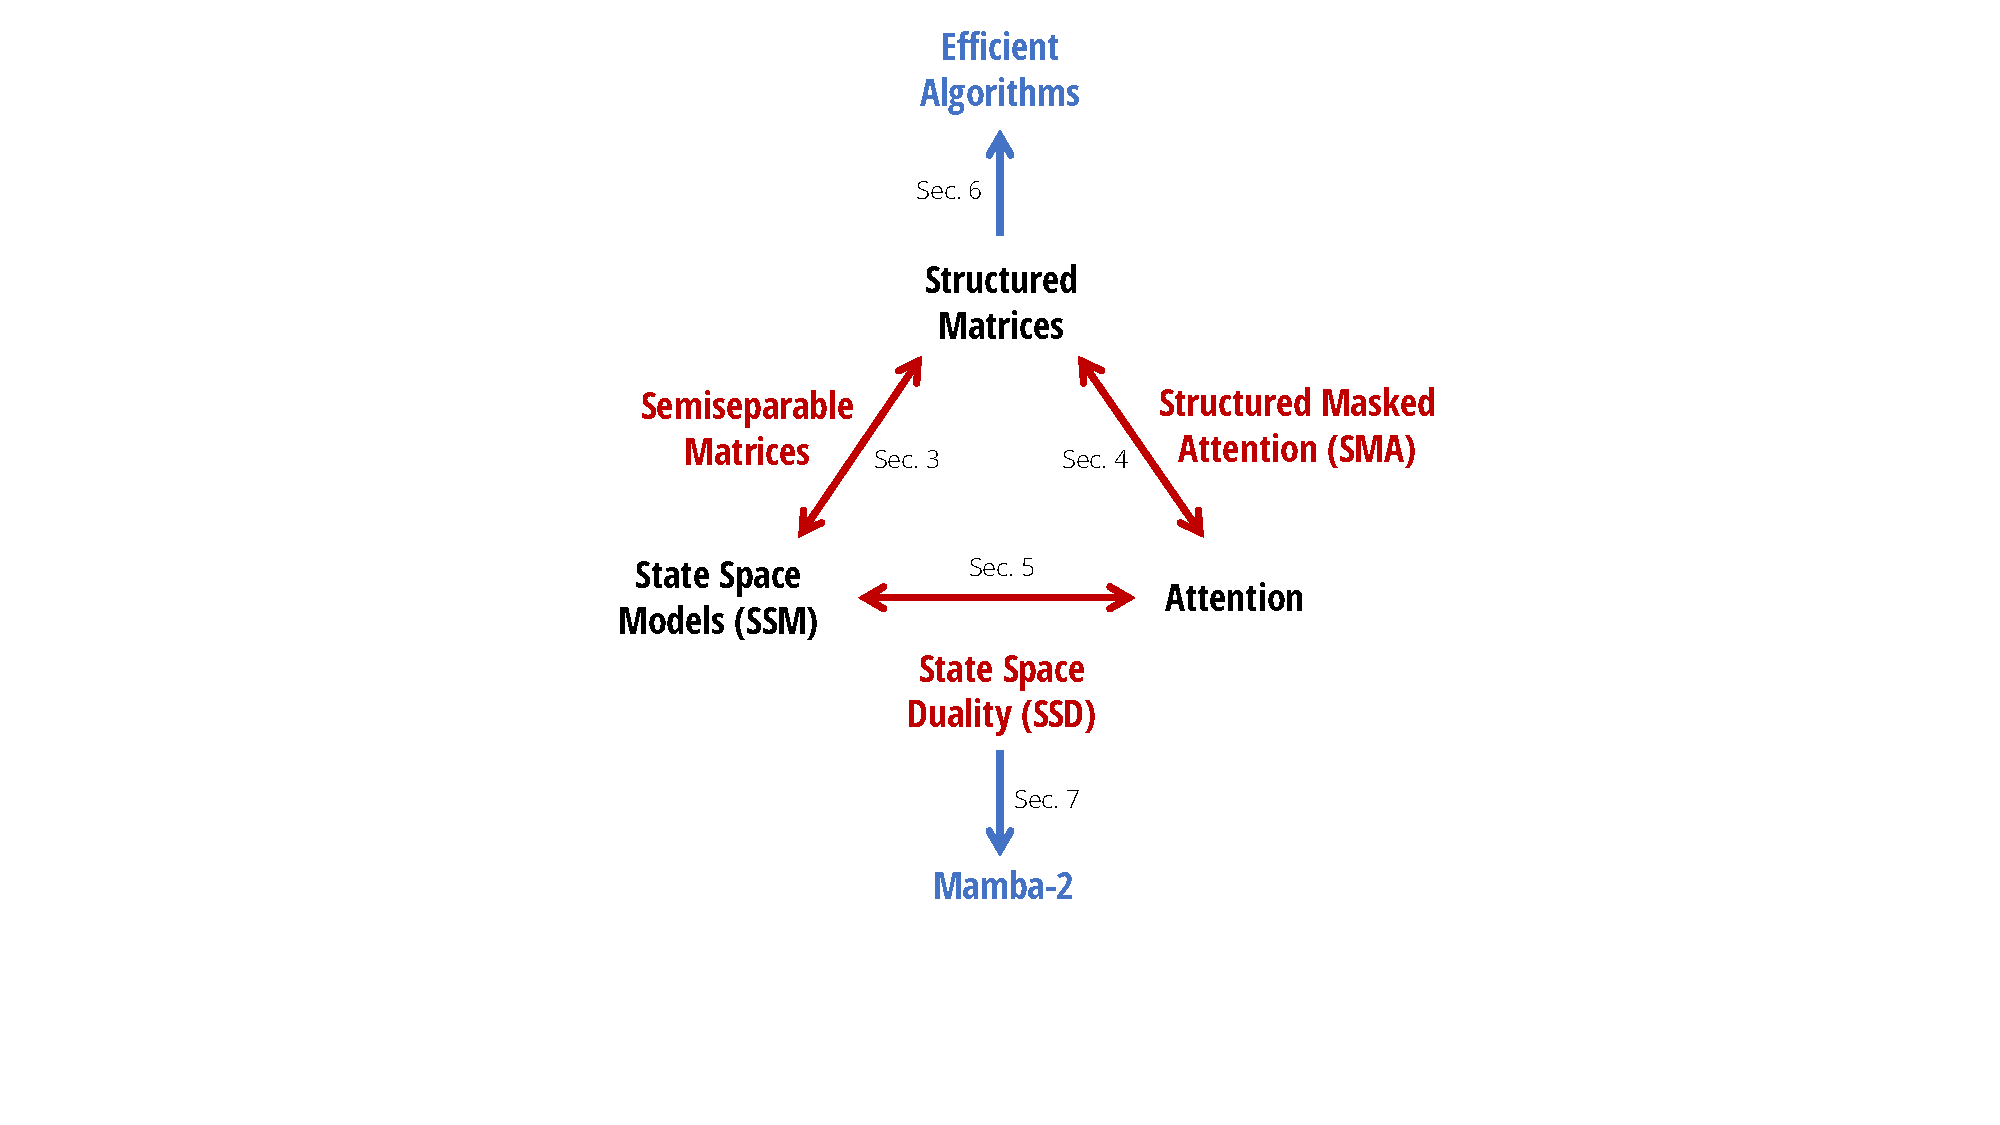
\includegraphics[width=\linewidth]{fig/ssd_roadmap.pdf}
  \end{center}
  \caption{
    (\textbf{Structured State-Space Duality}.)
    This paper fleshes out the relationship between state space models and attention through the bridge of structured matrices.
  }
  \label{fig:roadmap}
\end{wrapfigure}
}{}

\para{State Space Duality.}
Our framework connecting structured SSMs and variants of attention, which we call \textbf{structured state space duality} (SSD),
is made through the abstractions of \textbf{structured matrices}:
matrices with subquadratic parameters and multiplication complexity.
We develop two broad frameworks for representing sequence models, one as matrix transformations and one as tensor contractions, which each reveal different perspectives of the duality.
Our technical contributions include:
\begin{itemize}[leftmargin=*,itemsep=0pt,topsep=0pt]
  \item We show an equivalence between state space models and a well-studied family of structured matrices called \textbf{semiseparable matrices}\iftoggle{arxiv}{ (\cref{sec:ssm})}{}.
    This connection is at the heart our framework, revealing new properties and algorithms for SSMs. A central message of this paper is that \emph{different methods of computing state space models can be reframed as various matrix multiplication algorithms on structured matrices}.
  \item We significantly improve the theory of linear attention~\citep{katharopoulos2020transformers}.
    We first provide an incisive proof of its recurrent form through the language of tensor contractions, and then generalize it to a new family of \textbf{structured masked attention (SMA)}\iftoggle{arxiv}{ (\cref{sec:attention})}{}.
  \item We connect SSMs and SMA, showing that they have a large intersection that are duals of each other, possessing both SSM-like linear and attention-like quadratic forms\iftoggle{arxiv}{ (\cref{sec:ssd})}{}.
    \iftoggle{arxiv}{We also prove that any kernel attention method possessing a fast recurrent form must be an SSM.}{}
\end{itemize}


Beyond its intrinsic theoretical value, our framework opens up a broad set of directions for understanding and improving sequence models.

\para{Efficient Algorithms.}
First and most importantly, our framework exposes new efficient and easily-implementable algorithms for computing SSMs\iftoggle{arxiv}{ (\cref{sec:efficient})}{}.
We introduce a new \textbf{SSD algorithm}, based on block decompositions of semiseparable matrices, that takes advantage of both the linear SSM recurrence and quadratic dual form, obtaining optimal tradeoffs on all main efficiency axes (e.g. training and inference compute, memory usage, and ability to leverage matrix multiplication units on modern hardware).
A dedicated implementation of SSD is $2-8\times$ faster than the optimized selective scan implementation of Mamba, while simultaneously allowing for much larger recurrent state sizes ($8\times$ the size of Mamba or even higher, with minimal slowdown).
SSD is highly competitive with optimized implementations of softmax attention (FlashAttention-2~\citep{dao2023flashattention2}), crossing over at sequence length 2K and 6$\times$ faster at sequence length 16K.


\iftoggle{arxiv}{
\para{Architecture Design.}
One major obstacle to adopting new architectures such as SSMs is the ecosystem tailored to Transformers, such as hardware-efficient optimization and parallelism techniques for large-scale training.
Our framework allows using established conventions and techniques for attention to build a vocabulary of architecture design choices for SSMs, and further improve them (\cref{sec:architecture}).
For example, we introduce the analog of heads from multi-head attention (MHA) to SSMs.
We show that the Mamba architecture is a \textbf{multi-input SSM (MIS)} that turns out to be analogous to \textbf{multi-value attention (MVA)}, and compare other variants of Mamba with different head structures.

We also use these ideas to make slight modifications to the Mamba block, which allows tensor parallelism to be implemented (e.g. in the style of Megatron~\citep{shoeybi2019megatron}).
The main ideas include introducing grouped-value attention (GVA) head structure, and moving all data-dependent projections to occur in parallel at the beginning of the block.


}{
  \para{Mamba-2.}
  Additionally, inspired by the connection between SSMs and Transformers, we slightly modify the neural network architecture of Mamba by moving all data-dependent projections to occur in parallel at the beginning of the block. %
}
The combination of the modified parallel Mamba block, together with using SSD as the inner SSM layer, results in the \textbf{Mamba-2} architecture.
We investigate Chinchilla scaling laws for Mamba-2 in the same setting as Mamba, finding that it Pareto dominates Mamba and Transformer++ in both perplexity and wall-clock time.
We additionally train a family of Mamba-2 models at varying sizes on the Pile, showing that it matches or outperforms Mamba and open source Transformers on standard downstream evaluations.
For example, Mamba-2 with 2.7B parameters trained on 300B tokens on the Pile outperforms Mamba-2.8B, Pythia-2.8B and even Pythia-6.9B trained on the same dataset.

\iftoggle{arxiv}{
\paragraph{Systems Optimizations.}
The SSD framework connects SSMs and Transformers, allowing us to leverage a rich body of work on systems optimizations developed for Transformers~(\cref{sec:systems}).
\begin{itemize}[leftmargin=*,itemsep=0pt,topsep=0pt]
  \item For example, Tensor Parallelism (TP) is an important model parallelism technique to train large Transformer models by splitting each layer across GPUs on the same node.
    We design Mamba-2 to be TP-friendly, reducing the number of synchronization point per block by half.
  \item For very long sequences whose activations do not fit on one device, sequence parallelism has been developed for the attention blocks.
    We describe how to train SSMs in general and Mamba-2 in particular with sequence parallelism, by passing the recurrent states between devices.
  \item For finetuning with examples of different lengths, for best efficiency, Transformer requires sophisticated techniques to remove padding tokens and perform attention on variable length sequences.
    We show how Mamba-2 can be trained with variable sequence lengths efficiently, requiring no padding tokens.
\end{itemize}
}{}

\cref{sec:experiments} empirically validates Mamba-2 on language modeling, training efficiency, and a difficult multi-query associative recall task~\citep{arora2024simple}.
Finally, in \cref{sec:related}, we provide an extended related work and discuss potential research directions opened up by our framework.

Model code and pre-trained checkpoints are open-sourced at \url{https://github.com/state-spaces/mamba}.







%
\section{Related Work}
%


\subsection{Classical Approaches} \label{appendix:related_work_classical}

Classical approaches in time series modeling include the Box-Jenkins method \citep{box1968some}, exponential smoothing  \citep{hyndman2008forecasting, winters1960forecasting}, autoregressive integrated moving average (ARIMA) \citep{box1970time}, and state-space models \citep{hamilton1994state}. In such approaches, the model is usually manually selected based analyzing time series features (e.g., seasonality and order of non-stationarity), where the selected model is then fitted for each individual time series. While classical approaches may be more interpretable than recent deep learning techniques, the domain expertise and manual labor needed to succesfully apply them renders them infeasible to the common setting of modeling thousands, or millions, of time series.

\subsection{Deep Learning Approaches} \label{appendix:related_work_deep}

% (Deep AR, LSTMs, RNNs)
\textbf{Recurrent models.}  Common deep learning architectures for modeling sequence data are the family of recurrent neural networks, which include GRUs~\citep{chung2014empirical}, LSTMs~\citep{hochreiter1997long}, and DeepAR \citep{salinas2020deepar}. However, due to the recurrent nature of RNNs, they are slow to train and may suffer from vanishing/exploding gradients, making them difficult to train \citep{pascanu2013difficulty}. \\

\textbf{Deep State Space models.} Recent work has investigated combining the expressive strengths of SSMs with the scalable strengths of deep neural networks \citep{rangapuram2018, gu2021efficiently}. \cite{rangapuram2018} propose to train a global RNN that transforms input covariates to sequence-spcific SSM parameters; however, one downside of this approach is that they inherit the drawbacks of RNNs. More recent approaches, such as LSSL \citep{gu2021combining}, S4 \citep{gu2021efficiently}, S4D \citep{gu2022parameterization}, and S5 \citep{smith2022simplified}, directly parameterize the layers of a neural network with multiple linear SSMs, and overcome common recurrent training drawbacks by leveraging the convolutional view of SSMs. While deep SSM models have been shown great promise in time series modeling, we show in our work -- which builds off deep SSMs -- that current deep SSM approaches are not able to capture autoregressive processes due to their continuous nature.  \\


\textbf{Neural differential equations as nonlinear state spaces.}
%
\citep{chen2018neural} parametrizes the vector field of continuous--time autonomous systems. These models, termed \textit{Neural Differential Equations} (NDEs) have seen extensive application to time series and sequences, first by \cite{rubanova2019latent} and then by \cite{kidger2020neural,morrill2021neural,massaroli2021differentiable} with the notable extension to \textit{Neural Controlled Differential Equations} (Neural CDEs). Neural CDEs can be considered the continuous--time, nonlinear version of state space models and RNNs \citep{kidger2022neural}. Rather than introducing nonlinearity between linear state space layers, Neural CDEs model nonlinear systems driven by a control input. 

The NDE framework has been further applied by \cite{poli2019graph} to model graph time series via \textit{Neural Graph Differential Equations}. In \cite{queiruga2020continuous}, a continuous-depth ResNet generalization based on ODEs is proposed, and in \cite{kim2021stiff} numerical techniques to enable learning of stiff dynamical systems with Neural ODEs are investigated. The idea of parameterizing the vector field of a differential equation with a neural network, popularized by NDEs, can be traced back to earlier works \citep{funahashi1993approximation, zhang2014comprehensive, weinan2017proposal}. \\



\textbf{Transformers.} 
While RNNs and its variants have shown some success at time series modeling, a major limitation is their applicability to long input sequences. Since RNNs are recurrent by nature, they require long traversal paths to access past inputs, which leads to vanishing/exploding gradients and as a result struggle with capturing long-range dependencies. 

To counteract the long-range dependency problem with RNNs, a recent line of work considers Transformers for time series modeling. The motivation is that due to the attention mechanism, a Transformer can directly model dependencies between any two points in the input sequence, independently of how far apart the points are. However, the high expressivity of the attention mechanism comes at the cost of the time and space complexity being quadratic in sequence length, making Transformers infeasible for very long sequences. As a result, many works consider specialized Transformer architectures with sparse attention mechanisms to bring down the quadratic complexity. For example, \cite{beltagy2020longformer} propose LogSparse self-attention, where a cell attends to a subset of past cells (as opposed to all cells), where closer cells are attended to more frequently, proportional to the log of their distance, which brings down complexity from $\mathcal{O}(\ell^2)$ to $\mathcal{O}(\ell(\log \ell)^2)$. \cite{zhou2021informer} propose ProbSparse self-attention, which achieves $\mathcal{O}(\ell \log \ell)$ time and memory complexity, where they propose a generative style decoder to speed inference. \cite{liu2022pyraformer} propose a pyramidal attention mechanism which shows linear time and space complexity with sequence length. Autoformer \citep{wu2021autoformer} suggests more specialization is needed in time series with a decomposition forecasting architecture, which extracts long-term stationary trend from the seasonal series and utilizes an auto-correlation mechanism, which discovers the period-based dependencies. \cite{zhou2022fedformer} believes previous attempts of Transformer-based architectures do not capture global statistical properties, and to do so requires an attention mechanism in the frequency domain. Confromer \citep{gulati2020conformer} stacks convolutional and self-attention modules into a shared layer to combine the strengths of local interactions from convolutional modules and global interactions from self-attention modules. Perceiver AR \citep{hawthorne2022general} builds on the Perceiver architecture, which reduces the computational complexity of transformers by performing self-attention in a latent space, and extends Perceiver's applicability to causal autoregressive generation.

While these works have shown exciting progress on time series forecasting, their proposed architectures are specialized to handle specific time series settings (e.g., long input sequences, or seasonal sequences), and are commonly trained to output a fixed target horizon length \citep{zhou2021informer}, \ie{} as \emph{direct multi-step forecasting} (DMS) \cite{https://doi.org/10.1111/j.1467-6419.2007.00518.x}. Thus, while effective at specific forecasting tasks, their setups are not obviously applicable to a broad range of time series settings (such as forecasting arbitrary horizon lengths, or generalizing to classification or regression tasks).
%

Moreover, \cite{zeng2022transformers} showed that simpler alternatives to Transformers, such as data normalization plus a single linear layer (NLinear), can outperform these specialized Transformer architectures when similarly trained to predict the entire fixed forecasting horizons. Their results suggest that neither the attention mechanism nor the proposed modifications of these time series Transformers may be best suited for time series modeling. Instead, the success of these prior works  may just be from learning to forecast the entire horizon with fully connected dependencies between prior time-step inputs and future time-step outputs, where a fully connected linear layer is sufficient. \\

\textbf{Other deep learning methods.} Other works also investigate pure deep learning architectures with no explicit temporal components, and show these models can also perform well on time series forecasting. \cite{oreshkin2019n} propose N-BEATS, a deep architecture based on backward and forward residual links. Even simpler, \cite{zeng2022transformers} investigate single linear layer models for time series forecasting. Both works show that simple architectures are capable of achieving high performance for time series forecasting. In particular, with just data normalization, the NLinear model in \cite{zeng2022transformers} obtained state-of-the-art performance on the popular Informer benchmark~\cite{zhou2021informer}. Given an input sequence of past lag terms and a target output sequence of future horizon terms, for every horizon output their model simply learns the fully connected dependencies between that output and every input lag sample. However, FCNs such as NLinear also carry inefficient downsides. Unlike Transformers and SSM-based models, the number of parameters for FCNs scales directly with input and output sequence length, \ie{} $\mathcal{O}(\ell h)$ for $\ell$ inputs and $h$ outputs. Meanwhile, \ourmethod{} shows that the SSM can improve the modeling quality of deep architectures, while maintaining constant parameter count regardless of input or output length. Especially when forecasting long horizons, we achieve higher forecasting accuracy with smaller models.

% \header{S4}\\




\section{Methodology}
\ours follows the same framework as speculative decoding, where each decoding step primarily consists of three substeps: (1) generating candidates, (2) processing candidates, and (3) accepting candidates. For \ours, (1) is achieved by \ours heads, (2) is realized by tree attention, and since \ours heads are on top of the original model, the logits calculated in (2) can be used for substep (1) for the next decoding step. The final step (3) can be realized by either rejection sampling~\citep{leviathan2022fast,chen2023accelerating} or typical acceptance (Section~\ref{sec:typical_acceptance}). The overall pipeline is illustrated in Figure~\ref{fig:pipeline}.

In this section, we first introduce the key components of \ours, including \ours heads, and tree attention. Then, we present two levels of fine-tuning procedures for \ours to meet the needs of different use cases. Finally, we propose two extensions to \ours, including self-distillation and typical acceptance, to handle situations where no training data is available for \ours and to improve the efficiency of the decoding process, respectively.
\subsection{Key Components}
\subsubsection{\ours Heads}
\label{sec:medusa_heads}
In speculative decoding, subsequent tokens are predicted by an auxiliary draft model. This draft model must be small yet effective enough to generate continuations that the original model will accept. Fulfilling these requirements is a challenging task, and existing approaches~\citep{spector2023accelerating,miao2023specinfer} often resort to separately \emph{pre-training} a smaller model. This pre-training process demands substantial additional computational resources. For example, in \citep{miao2023specinfer}, a reported 275 NVIDIA A100 GPU hours were used. Additionally, separate pre-training can potentially create a distribution shift between the draft model and the original model, leading to continuations that the original model may not favor. \citet{chen2023accelerating} have also highlighted the complexities of serving multiple models in a distributed environment.

\textcolor{black}{To streamline and democratize the acceleration of LLM inference, we take inspiration from \citet{stern2018blockwise}, which utilizes parallel decoding for tasks such as machine translation and image super-resolution. \ours heads}
 are additional decoding heads appended to the last hidden states of the original model. Specifically, given the original model's last hidden states $h_t$ at position $t$, we add $K$ decoding heads to $h_t$. The $k$-th head is used to predict the token in the $(t+k+1)$-th position of the next tokens (the original language model head is used to predict the $(t+1)$-th position). The prediction of the $k$-th head is denoted as $p_t^{(k)}$, representing a distribution over the vocabulary, while the prediction of the original model is denoted as $p_t^{(0)}$. Following the approach of \citet{stern2018blockwise}, we utilize a single layer of feed-forward network with a residual connection for each head. We find that this simple design is sufficient to achieve satisfactory performance. The definition of the $k$-th head is outlined as:

\begin{align*}
p_t^{(k)} = \text{softmax}\left(W_2^{(k)} \cdot \left(\text{SiLU}(W_1^{(k)} \cdot h_t)+h_t\right)\right),\\
\text{where } W_2^{(k)}\in\mathbb{R}^{d\times V}, W_1^{(k)}\in\mathbb{R}^{d\times d}.
\end{align*}

\textcolor{black}{$d$ is the output dimension of the LLM's last hidden layer and $V$ is the vocabulary size.}
\textcolor{black}{We initialize $W_2^{(k)}$ identically to the original language model head, and $W_1^{(k)}$ to zero.}
This aligns the initial prediction of \ours heads with that of the original model. The SiLU activation function~\citep{elfwing2017sigmoidweighted} is employed following the Llama models~\citep{touvron2023llama}.

Unlike a draft model, \ours heads are trained in conjunction with the original backbone model, which can remain \emph{frozen} during training (\ours-1) or be trained together (\ours-2). This method allows for fine-tuning large models even on a single GPU, taking advantage of the powerful base model's learned representations. Furthermore, it ensures that the distribution of the \ours heads aligns with that of the original model, thereby mitigating the distribution shift problem. Additionally, since the new heads consist of just a single layer akin to the original language model head, \ours does not add complexity to the serving system design and is friendly to distributed settings. We will discuss the training recipe for \ours heads in Section~\ref{sec:training_recipe}.

\subsubsection{Tree Attention}
\label{sec:tree_attention}
Through \ours heads, we obtain probability predictions for the subsequent $K+1$ tokens. These predictions enable us to create length-$K+1$ continuations as candidates. While the speculative decoding studies~\citep{leviathan2022fast,chen2023accelerating} suggest sampling a single continuation as the candidate, leveraging multiple candidates during decoding can enhance the expected acceptance length within a decoding step. Nevertheless, more candidates can also raise computational demands. To strike a balance, we employ a tree-structured attention mechanism to process multiple candidates concurrently.
\begin{figure}[ht]
    \centering
    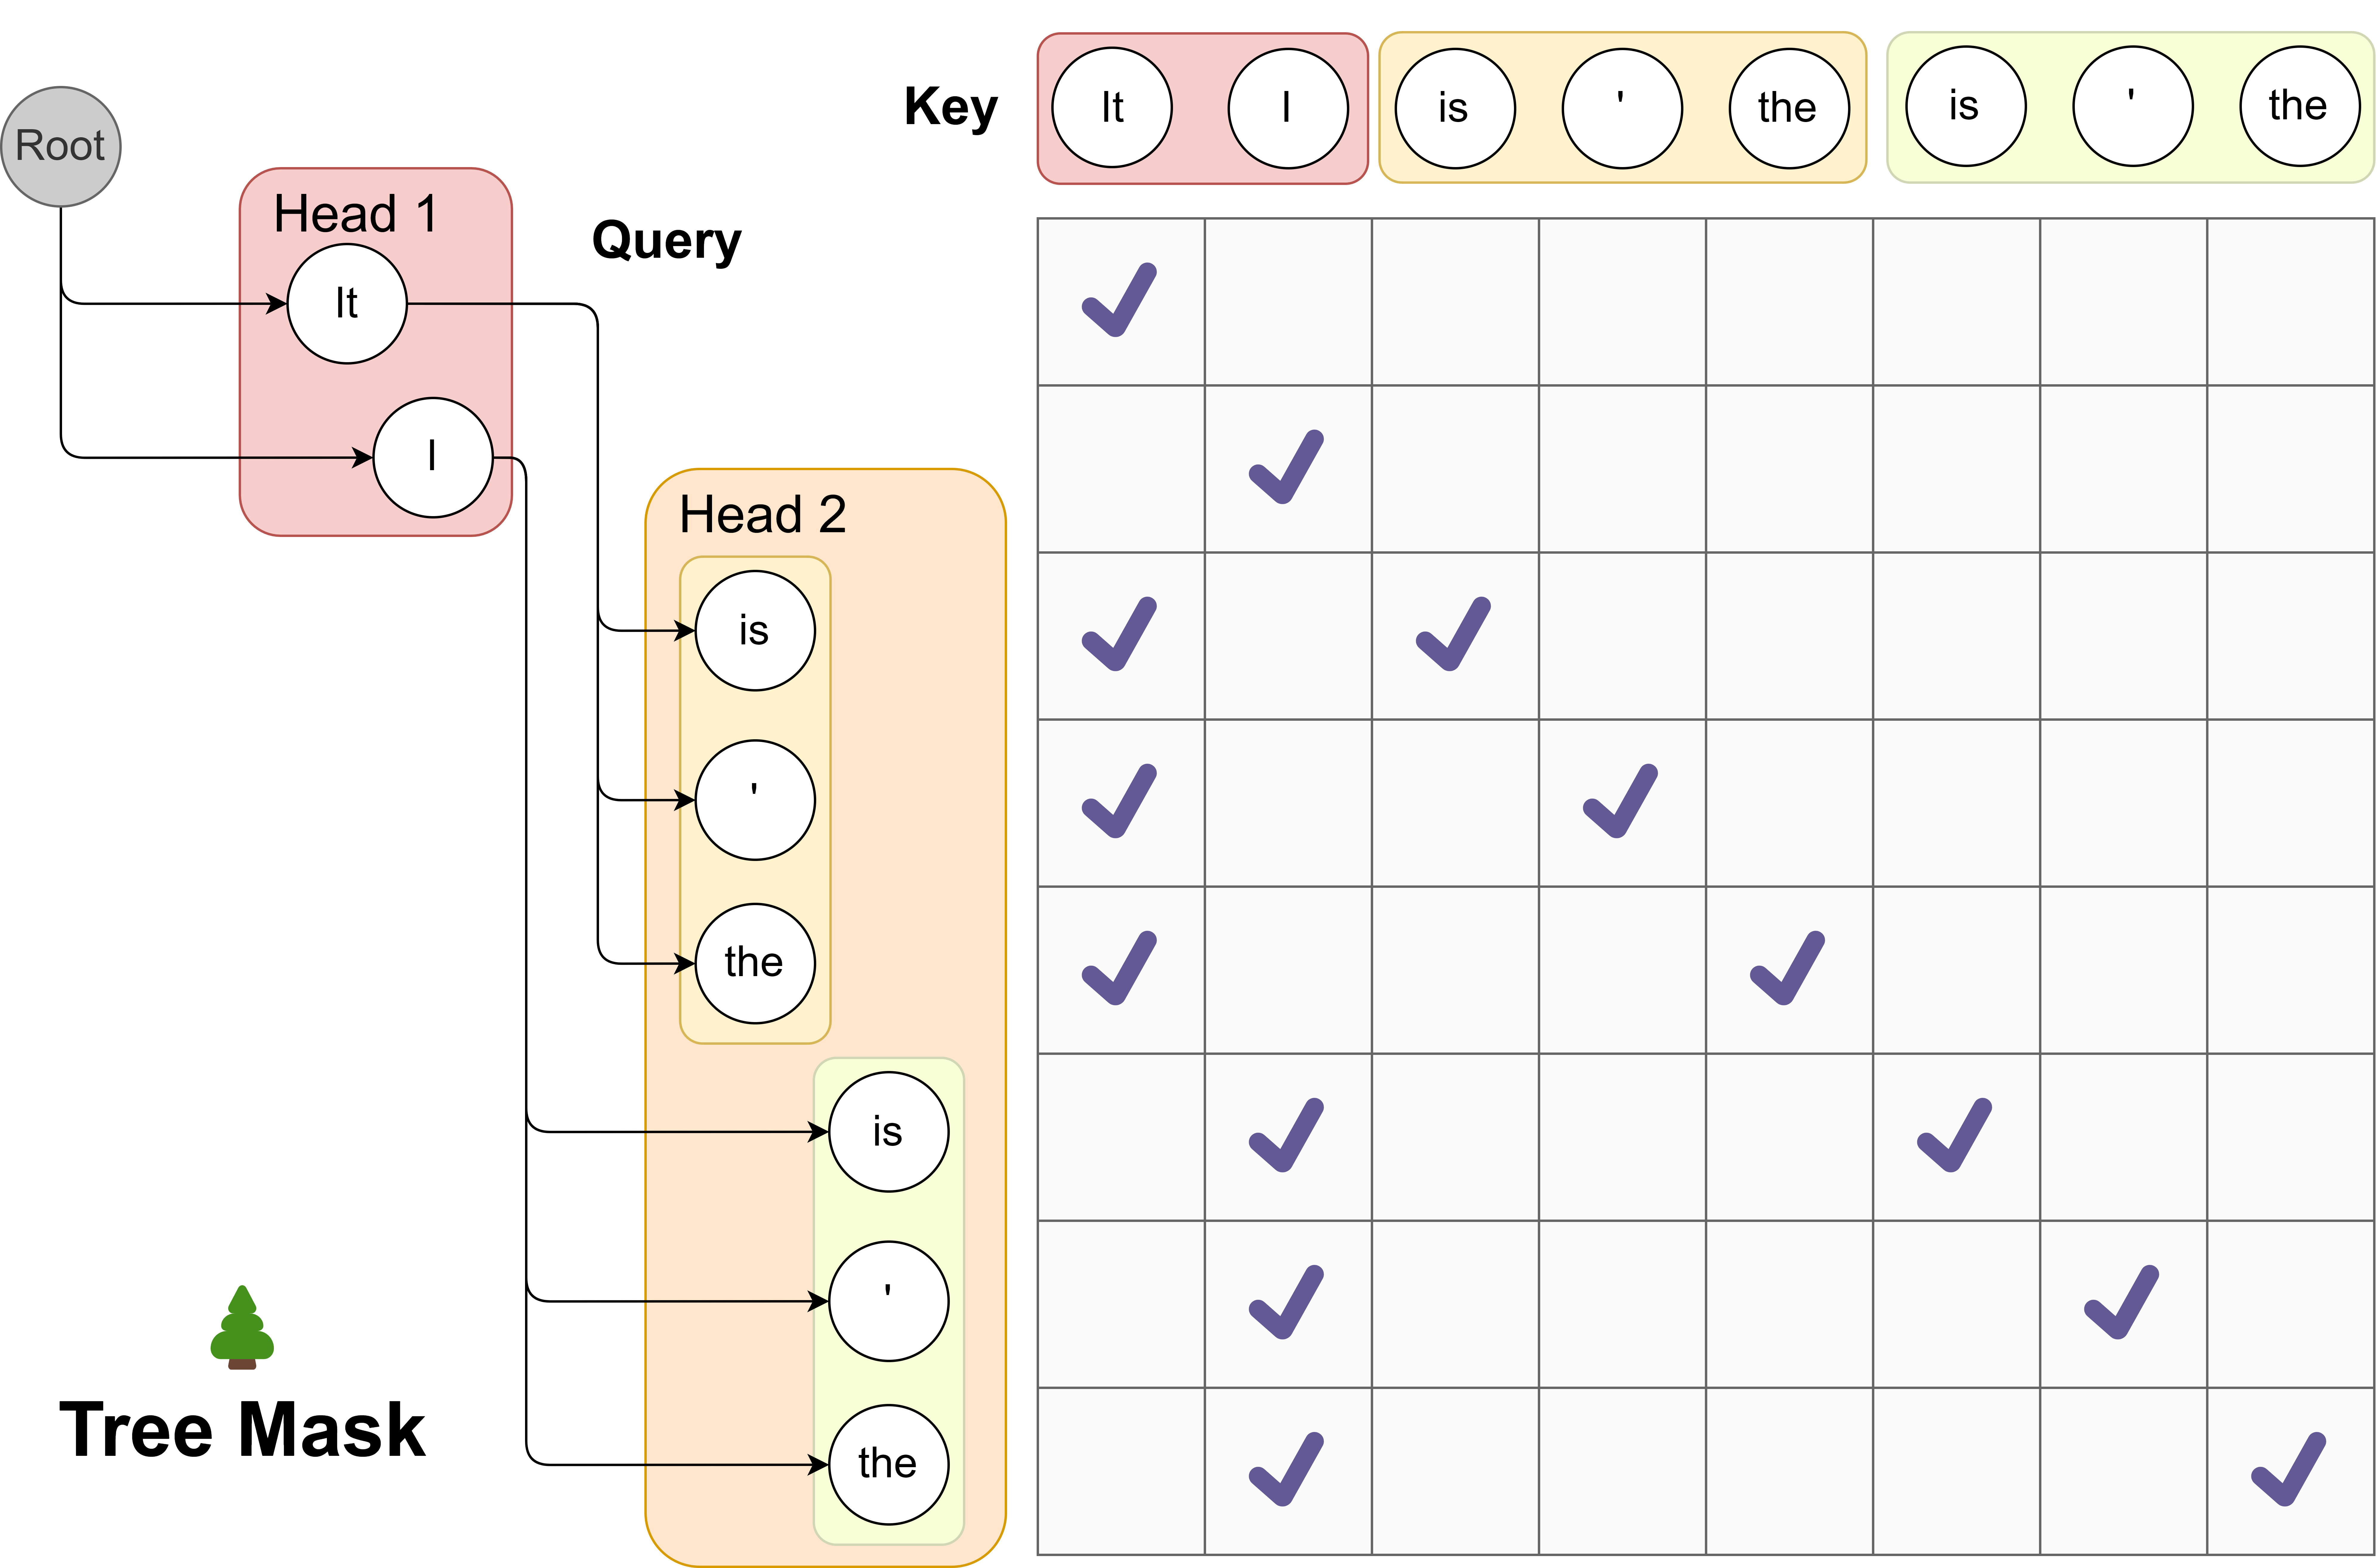
\includegraphics[width=0.45\textwidth]{tree_attention.png}
    \caption{
    We demonstrates the use of tree attention to process multiple candidates concurrently. As exemplified, the top-2 predictions from the first \ours head and the top-3 from the second result in a total of $2\times3=6$ candidates. Each of these candidates corresponds to a distinct branch within the tree structure. To guarantee that each token only accesses its predecessors, we devise an attention mask that exclusively permits attention flow from the current token back to its antecedent tokens. The positional indices for positional encoding are adjusted in line with this structure.}
    \label{fig:tree_attention}
\end{figure}
This attention mechanism diverges from the traditional causal attention paradigm. Within this framework, only tokens from the same continuation are regarded as historical data. Drawing inspiration from the concept of embedding graph structures into attention as proposed in the graph neural network domain~\citep{ying2021transformers}, we incorporate the tree structure into our attention mask, visualized in Figure~\ref{fig:tree_attention}. Remarkably, similar ideas have also been explored in independent works like \citet{miao2023specinfer,spector2023accelerating}, where they follow a bottom-up approach and construct the tree by merging multiple candidates generated by a draft model. In our method, we instead take a top-down approach to build the tree thanks to the structure of candidates generated by \ours heads. For a given $k$-th head, its top-$s_k$ predictions serve as the basis for candidate formation, where $s_k$ is a designated hyperparameter. These candidates are established by determining the Cartesian product of the top-$s_k$ predictions from each head. For instance, in Figure~\ref{fig:tree_attention}, with $s_1=2$ and $s_2=3$, each first head prediction can be succeeded by any prediction from the second head. This leads to a tree structure where $s_k$ branches exist at the $k$-th level (considering a virtual root as the $0$-level, in practice, this $0$-level is for the prediction of the language model head of the original model, which can be sampled independently). Within this tree, only a token's predecessors are seen as historical context, and our attention mask ensures that the attention is only applied on a token's predecessors. By employing this mask and properly setting the positional indices for positional encoding, we can process numerous candidates simultaneously without the need to expand the batch size. The cumulative number of new tokens is calculated as $\sum_{k=1}^K \prod_{i=1}^k s_i$.

In this section, we demonstrate the most simple and regular way to construct the tree structure by taking the Cartesian product. However, it is possible to construct the tree structure in a more sophisticated way and exploit the unbalanced accuracy of different top predictions of different heads. We will discuss this in Section~\ref{sec:optimized_tree_construction}.
\subsection{Training Strategies}
\label{sec:training_recipe}
At the most basic level, we can train \ours heads by freezing the backbone model and fine-tuning \ours heads. However, training the backbone in conjunction with the \ours heads can significantly enhance the accuracy of the \ours heads. Depending on the computational resources and the specific reqirements of the use case, we propose two levels of training strategies for \ours heads.

In this section, we assume the availability of a training dataset that aligns with the target model’s output distribution. This could be the dataset used for Supervised Fine-Tuning (SFT) of the target model. We will discuss eliminating the need for such a dataset using a self-distillation approach in Section~\ref{sec:self_distillation}.
\subsubsection{\ours-1: Frozen Backbone}
\label{sec:frozen_backbone}
To train \ours heads with a frozen backbone model, we can use the cross-entropy loss between the prediction of \ours heads and the ground truth. Specifically, given the ground truth token $y_{t+k+1}$ at position $t+k+1$, the loss for the $k$-th head is $\mathcal{L}_k = -\log p_t^{(k)}(y_{t+k+1})$ where $p_t^{(k)}(y)$ denotes the probability of token $y$ predicted by the $k$-th head. We also observe that $\mathcal{L}_k$ is larger when $k$ is larger, which is reasonable since the prediction of the $k$-th head is more uncertain when $k$ is larger. Therefore, we can add a weight $\lambda_k$ to $\mathcal{L}_k$ to balance the loss of different heads. And the total \ours loss is:
\begin{align}
    \label{eq:loss_medusa_1}
    \mathcal{L}_{\text{\ours-1}} = \sum_{k=1}^K -\lambda_k\log p_t^{(k)}(y_{t+k+1}).
\end{align}

In practice, we set $\lambda_k$ as the $k$-th power of a constant like $0.8$. Since we only use the backbone model for providing the hidden states, we can use a quantized version of the backbone model to reduce the memory consumption. This introduces a more democratized way to accelerate LLM inference, as with the quantization, \ours can be trained for a large model on a single consumer GPU similar to QLoRA~\citep{dettmers2023qlora}. The training only takes a few hours (e.g., 5 hours for \ours-1 on Vicuna 7B model with a single NVIDIA A100 PCIE GPU to train on 60k ShareGPT samples).
\subsubsection{\ours-2: Joint Training}
\label{sec:joint_training}
To further improve the accuracy of \ours heads, we can train \ours heads together with the backbone model. However, this requires a special training recipe to preserve the backbone model's next-token prediction capability and output quality. To achieve this, we propose three strategies:
\begin{itemize}
    \item \textbf{Combined loss}: To keep the backbone model's next-token prediction capability, we need to add the cross-entropy loss of the backbone model $\mathcal{L}_{\text{LM}}=-\log p_t^{(0)}(y_{t+1})$ to the \ours loss. We also add a weight $\lambda_0$ to balance the loss of the backbone model and the \ours heads. Therefore, the total loss is:
    \begin{align}
        \label{eq:loss_medusa_2}
        \mathcal{L}_{\text{\ours-2}} = \mathcal{L}_{\text{LM}} + \lambda_0\mathcal{L}_{\text{\ours-1}}.
    \end{align}
    \item \textbf{Differential learning rates}: Since the backbone model is already well-trained and the \ours heads need more training, we can use separate learning rates for them to enable faster convergence of \ours heads while preserving the backbone model's capability.
    \item \textbf{Heads warmup}: Noticing that at the beginning of training, the \ours heads have a large loss, which leads to a large gradient and may distort the backbone model's parameters. Following the idea from \citet{kumar2022finetuning}, we can employ a two-stage training process. In the first stage, we only train the \ours heads as \ours-1. In the second stage, we train the backbone model and \ours heads together with a warmup strategy. Specifically, we first train the backbone model for a few epochs, then train the \ours heads together with the backbone model. Besides this simple strategy, we can also use a more sophisticated warmup strategy by gradually increasing the weight $\lambda_0$ of the backbone model's loss. We find both strategies work well in practice.
\end{itemize}
Putting these strategies together, we can train \ours heads together with the backbone model without hurting the backbone model's capability. Moreover, this recipe can be applied together with Supervised Fine-Tuning (SFT), enabling us to get a model with native \ours support.
\subsubsection{How to Select the Number of Heads}
Empirically, we found that five heads are sufficient at most. Therefore, we recommend training with five heads and referring to the strategy described in Section~\ref{sec:optimized_tree_construction} to determine the optimal configuration of the tree attention. With optimized tree attention, sometimes three or four heads may be enough for inference. In this case, we can ignore the redundant heads without overhead.

\subsection{Extensions}
\subsubsection{Typical Acceptance}
\label{sec:typical_acceptance}
In speculative decoding papers~\citep{leviathan2022fast,chen2023accelerating}, authors employ rejection sampling to yield diverse outputs that align with the distribution of the original model. However, subsequent implementations~\citep{gante2023assisted,spector2023accelerating} reveal that this sampling strategy results in diminished efficiency as the sampling temperature increases. Intuitively, this can be comprehended in the extreme instance where the draft model is the same as the original one\textcolor{black}{:} 
Using greedy decoding, all output of the draft model will be accepted, therefore maximizing the efficiency. 
Conversely, rejection sampling introduces extra overhead, as the draft model and the original model are sampled independently. Even if their distributions align perfectly, the output of the draft model may still be rejected.

However, in real-world scenarios, sampling from language models is often employed to generate diverse responses, and the temperature parameter is used merely to modulate the ``creativity'' of the response. Therefore, higher temperatures should result in more opportunities for the original model to accept the draft model's output. We ascertain that it is typically unnecessary to match the distribution of the original model. Thus, we propose employing a \emph{typical acceptance} scheme to select plausible candidates rather than using rejection sampling. This approach draws inspiration from truncation sampling studies~\citep{hewitt2022truncation} (refer to \textcolor{black}{Appendix}~\ref{sec:related_work} for an in-depth explanation). Our objective is to choose candidates that are \emph{typical}, meaning they are not exceedingly improbable to be produced by the original model. We use the prediction probability from the \emph{original model} as a natural gauge for this and establish a threshold based on the prediction distribution to determine acceptance. Specifically, given $x_1, x_2, \cdots, x_n$ as context, when evaluating the candidate sequence \textcolor{black}{$(x_{n+1}, x_{n+2}, \cdots, x_{n+K+1})$ }(composed by top predictions of the original language model head and \ours heads), we consider the condition
\begin{align*}
p_{\text{original}}(x_{n+k}|x_1, x_2, \cdots, x_{n+k-1}) > \\\min\rbr{\epsilon, \delta\exp\rbr{-H(p_{\text{original}}(\cdot|x_1, x_2, \cdots, x_{n+k-1}))}},
\end{align*}
where $H(\cdot)$ denotes the entropy function, and $\epsilon, \delta$ are \textcolor{black}{the hard threshold and the entropy-dependent
threshold respectively}. This criterion is adapted from \citet{hewitt2022truncation} and rests on two observations: (1) tokens with relatively high probability are meaningful, and (2) when the distribution's entropy is high, various continuations may be deemed reasonable. During decoding, every candidate is evaluated using this criterion, and a \emph{prefix} of the candidate is accepted if it satisfies the condition. To guarantee the generation of at least one token at each step, we apply \emph{greedy decoding} for the first token and \emph{unconditionally} accept it while employing typical acceptance for subsequent tokens. The final prediction for the current step is determined by the \emph{longest accepted prefix} among all candidates.

Examining this scheme leads to several insights. Firstly, when the temperature is set to $0$, it reverts to greedy decoding, as only the most probable token possesses non-zero probability. As the temperature surpasses $0$, the outcome of greedy decoding will consistently be accepted with appropriate $\epsilon, \delta$, since those tokens have the maximum probability, yielding maximal speedup. Likewise, in general scenarios, an increased temperature will correspondingly result in longer accepted sequences, as corroborated by our experimental findings.

Empirically, we verify that typical acceptance can achieve a better speedup while maintaining a similar \textcolor{black}{generation quality} as shown in Figure~\ref{fig:threshold_ablation}.
\subsubsection{Self-Distillation}
\label{sec:self_distillation}
In Section~\ref{sec:training_recipe}, we assume the existence of a training dataset that matches the target model's output distribution. However, this is not always the case. For example, the model owners may only release the model without the training data, or the model may have gone through a Reinforcement Learning with Human Feedback (RLHF) procedure, which makes the output distribution of the model different from the training dataset. To tackle this issue, we propose an automated self-distillation pipeline to use the model itself to generate the training dataset for \ours heads, which matches the output distribution of the model.

The dataset generation process is straightforward. We first take a public seed dataset from a domain similar to the target model; for example, using the ShareGPT~\citep{sharegpt2023} dataset for chat models. Then, we simply take the prompts from the dataset and ask the model to reply to the prompts. In order to obtain multi-turn conversation samples, we can sequentially feed the prompts from the seed dataset to the model. Or, for models like Zephyr 7B~\citep{tunstall2023zephyr}, which are trained on both roles of the conversation, they have the ability to self-talk, and we can simply feed the first prompt and let the model generate multiple rounds of conversation.

For \ours-1, this dataset is sufficient for training \ours heads. However, for \ours-2, we observe that solely using this dataset for training the backbone and \ours heads usually leads to a lower generation quality. In fact, even without training \ours heads, training the backbone model with this dataset will lead to performance degradation. This suggests that we also need to use the original model's probability prediction instead of using the ground truth token as the label for the backbone model, similar to classic knowledge distillation works~\citep{kim2016sequencelevel}. Concretely, the loss for the backbone model is:
\begin{align*}
    \mathcal{L}_{\text{LM-distill}} = KL(p_{\text{original},t}^{(0)}||p_t^{(0)}),
\end{align*}
where $p_{\text{original},t}^{(0)}$ denotes the probability distribution of the original model's prediction at position $t$.

However, naively, to obtain the original model's probability prediction, we need to maintain two models during training, increasing the memory requirements. To further alleviate this issue, we propose a simple yet effective way to exploit the self-distillation setup. We can use a parameter-efficient adapter like LoRA~\citep{hu2021lora} for fine-tuning the backbone model. In this way, the original model is simply the model with the adapter turned off. Therefore, the distillation does not require additional memory consumption. Together, this self-distillation pipeline can be used to train \ours-2 without hurting the backbone model's capability and introduce almost no additional memory consumption. Lastly, one tip about using self-distillation is that it is preferable to use LoRA without quantization in this case, otherwise, the teacher model will be the quantized model, which may lead to a lower generation quality.

\subsubsection{Searching for the Optimized Tree Construction}
\label{sec:optimized_tree_construction}
In Section~\ref{sec:tree_attention}, we present the simplest way to construct the tree structure by taking the Cartesian product. However, with a fixed budget for the number of total nodes in the tree, a regular tree structure may not be the best choice. Intuitively, those candidates composed of the top predictions of different heads may have different accuracies. Therefore, we can leverage an estimation of the accuracy to construct the tree structure.

Specifically, we can use a calibration dataset and calculate the accuracies of the top predictions of different heads. Let $a_k^{(i)}$ denote the accuracy of the $i$-th top prediction of the $k$-th head\footnote{Here, the accuracy is defined for the single top $i$-th token, i.e., this accuracy is equal to top-$i$ accuracy minus top-$(i-1)$ accuracy.}. Assuming the accuracies are independent, we can estimate the accuracy of a candidate sequence composed by the top $\sbr{i_1, i_2, \cdots, i_k}$ predictions of different heads as $\prod_{j=1}^k a_j^{(i_j)}$. Let $I$ denote the set of all possible combinations of $\sbr{i_1, i_2, \cdots, i_k}$ and each element of $I$ can be mapped to a node of the tree (not only leaf nodes but all nodes are included). Then, the expectation of the acceptance length of a candidate sequence is:
\begin{align*}
    \sum_{\sbr{i_1, i_2, \cdots, i_k}\in I}\prod_{j=1}^k a_j^{(i_j)}.
\end{align*}
Thinking about building a tree by adding nodes one by one, the contribution of a new node to the expectation is exactly the accuracy associated with the node. Therefore, we can greedily add nodes to the tree by choosing the node that is connected to the current tree and has the highest accuracy. This process can be repeated until the total number of nodes reaches the desired number. In this way, we can construct a tree that maximizes the expectation of the acceptance length. Further details can be found in Appendix~\ref{appendix:sparse_tree}.



\vspace{-0.2cm}
\section{Experiments Details}
\label{sec:exp}

\vspace{-0.2cm}
\subsection{Roadmap Insights on FFHQ-256\texorpdfstring{~\cite{sg1}}{}}
\label{sub:arc-experiments}
\vspace{-0.1cm}
As per Table~\ref{tab:roadmap}, Config A (vanilla StyleGAN2) achieves an FID of 7.52 using the official implementation on FFHQ-256. Config B with all tricks removed achieves an FID of 12.46---performance drops as expected. 
Config C, with a well-behaved loss, achieves an FID of 11.65. But, now training is sufficiently stable to improve the architecture.

Config D, which improves $G$ and $D$ based on the classic ResNet and ConvNeXt findings, achieves an FID of 9.95. The output skips of the StyleGAN2 generator are no longer useful given our new architecture; including them produces a worse FID of 10.17. Karras~\etal find that the benefit of output skips is mostly related to gradient magnitude dynamics~\cite{sg3}, and this has been addressed by our ResNet architecture. For StyleGAN2, Karras~\etal conclude that a ResNet architecture is harmful to $G$~\cite{sg2}, but this is not true in our case as their ResNet implementation is considerably different from ours: 1) Karras~\etal use one 3-3 residual block for each resolution stage, while we have a separate transition layer and two 1-3-1 residual blocks; 2) i.3) and i.4) are violated as they do not have a linear residual block~\cite{mobnet} and the transition layer is placed on the skip branch of the residual block rather than the stem; 3) the essential principle of ResNet~\cite{resnet}---identity mapping~\cite{resnet2}---is violated as Karras~\etal divide the output of the residual block by $\sqrt{2}$ to avoid variance explosion due to the absence of a proper initialization scheme.

For Config E, we conduct two experiments that ablate i.\ref{item:i1} (increased width with depthwise conv.) and i.\ref{item:i2} (an inverted bottleneck). We add GroupedConv and reduce the bottleneck compression ratio to two given the same model size. Each bottleneck is now 1.5$\times$ the width of Config A, and the FID drops to 7.51, surpassing the performance of StyleGAN2. By inverting the stem and the bottleneck dimensions to enhance the capacity of GroupedConv, our final model achieves an FID of 7.05, exceeding StyleGAN2.


\begin{wraptable}[12]{r}{6.5cm}
\vspace{-1.25cm}
\centering
\caption{StackedMNIST 1000-mode coverage.}
% Our model outperforms other GANs in terms of $D_\text{KL}$, indicating that we are better able to recover the distribution.}
\vspace{-0.4cm}
\resizebox{0.8\linewidth}{!}{
\begin{tblr}{
  cell{2}{2} = {c},
  cell{2}{3} = {c},
  cell{3}{2} = {c},
  cell{3}{3} = {c},
  cell{4}{2} = {c},
  cell{4}{3} = {c},
  cell{5}{2} = {c},
  cell{5}{3} = {c},
  cell{6}{2} = {c},
  cell{6}{3} = {c},
  cell{7}{2} = {c},
  cell{7}{3} = {c},
  cell{8}{2} = {c},
  cell{8}{3} = {c},
  cell{9}{2} = {c},
  cell{9}{3} = {c},
  cell{10}{2} = {c},
  cell{10}{3} = {c},
  cell{11}{2} = {c},
  cell{11}{3} = {c},
  cell{12}{2} = {c},
  cell{12}{3} = {c},
  hline{2,12} = {1-3}{},
}
Model     & \# modes$\uparrow$ & $D_\text{KL}$$\downarrow$            &  \\
DCGAN~\cite{dcgan}     & 99            & 3.40\phantom{0}&  \\
VEEGAN~\cite{srivastava2017veegan}    & 150           & 2.95\phantom{0}&  \\
WGAN-GP~\cite{wgan-gp}& 959           & 0.73\phantom{0}&  \\
PacGAN~\cite{pacgan}    & 992           & 0.28\phantom{0}&  \\
StyleGAN2~\cite{sg2} & 940           & 0.42\phantom{0}&  \\
PresGAN~\cite{presgan}   & \textbf{1000} & 0.12\phantom{0}&  \\
Adv. DSM~\cite{advsm}  & \textbf{1000} & 1.49\phantom{0}&  \\
VAEBM~\cite{vaebm}     & \textbf{1000} & 0.087          &  \\
DDGAN~\cite{ddgan}     & \textbf{1000} & 0.071          &  \\
MEG~\cite{meg}       & \textbf{1000} & 0.031          &  \\
Ours---Config E     & \textbf{1000} & \textbf{0.029} &  
\end{tblr}
}
\label{tab:stackedmnist}
\end{wraptable}%

\subsection{Mode Recovery --- StackedMNIST\texorpdfstring{~\cite{metz2016unrolled}}{}} 
\vspace{-0.1cm}
We repeat the earlier experiment in 1000-mode convergence on StackedMNIST (unconditional generation), but this time with our updated architecture and with comparisons to SOTA GANs and likelihood-based methods (Tab.~\ref{tab:stackedmnist}, Fig.~\ref{fig:stacked-mnist}). 
One advantage brought up of likelihood-based models such as diffusion over GANs is that they achieve mode coverage~\cite{adm}. We find that most GANs struggle to find all modes. But, PresGAN~\cite{presgan}, DDGAN~\cite{ddgan}, and our approach are successful. Further, our method outperforms all other tested GAN models in term of KL divergence.

\subsection{FID --- FFHQ-256\texorpdfstring{~\cite{sg1}}{} (Optimized)}
\vspace{-0.1cm}
We train Config E model until convergence and with optimized hyperparameters and training schedule on FFHQ at 256$\times$256 (unconditional generation) (Tab.~\ref{tab:ffhq256}, Figs.~\ref{fig:ffhq-256-teaser} and~\ref{fig:ffhq-256}). 
Please see our supplemental material for training details.
%The hyperparameters and schedule are listed in the supplemental material. 
Our model outperforms existing StyleGAN methods, plus four more recent diffusion-based methods. On this common dataset experimental setting, many methods (not listed here) use the bCR~\cite{zhao2021improved} trick---this has only been shown to improve performance on FFHQ-256 (not even at different resolutions of FFHQ)~\cite{zhao2021improved, zhang2022styleswin}. We do not use this trick. 
% no such tricks in our method.
% JT Try to minimize embellishment...
% This is particularly impressive given the fact that the dataset FFHQ was designed for StyleGAN~\cite{sg1} and the StyleGAN series of models were optimized with this specific dataset in mind.
% to achieve this performance.

\subsection{FID --- FFHQ-64\texorpdfstring{~\cite{edm}}{}}
\vspace{-0.1cm}
To compare with EDM~\cite{edm} directly, we evaluate our model on FFHQ at 64$\times$64 resolution. For this, we remove the two highest resolution stages of our 256$\times$256 model, resulting in a generator that is less than half the number of parameters as EDM. Despite this, our model outperforms EDM on this dataset and needs one function evaluation only (Tab.~\ref{tab:ffhq64}).

\begin{figure}
\begin{floatrow}
    %\hspace{-0.75cm}%
    \capbtabbox{%
        \centering
        \resizebox{\linewidth}{!}{
        \begin{tblr}{
          column{2,3} = {r},
          cell{1}{2} = {c},
          cell{1}{3} = {c},
          hline{2,5,9,10} = {-}{},
        }
        Model       & NFE$\downarrow$ & FID$\downarrow$  \\
        StyleGAN2~\cite{sg2}   & 1               & 3.78 \\
        StyleGAN3-T~\cite{sg3} & 1               & 4.81 \\
        StyleGAN3-R~\cite{sg3} & 1               & 3.92 \\
        LDM~\cite{rombach2022high} & 200               & 4.98\\
        ADM (DDIM)~\cite{adm,compdiff} & 500               & 8.41\\
        ADM (DPM-Solver)~\cite{adm,compdiff} & 500               & 8.40\\
        Diffusion Autoencoder~\cite{diffae,compdiff} & 500               & 5.81\\
        Ours---Config E  & 1               & 2.75 \\
        \emph{With ImageNet feature leakage~\cite{kynkaanniemi2022role}:} & & \\
        PolyINR*~\cite{singh2023polynomial} & 1               & 2.72 \\
        StyleGAN-XL*~\cite{sgxl} & 1               & 2.19 \\
        StyleSAN-XL*~\cite{takida2024san} & 1               & 1.68 \\
        \end{tblr}
        }
    }{%
        \caption{
        \label{tab:ffhq256}FFHQ-256. * denotes models that leak ImageNet features.}
    }
    %
    \capbtabbox{%
        \centering
        \resizebox{0.85\linewidth}{!}{
        \begin{tblr}{
          column{2} = {r},
          column{3} = {r},
          hline{2,5,8} = {-}{},
        }
        Model         & NFE$\downarrow$ & FID$\downarrow$ \\
        StyleGAN2~\cite{sg2,anycostgan}     & 1               & 3.32            \\
        MSG-GAN~\cite{karnewar2020msg,anycostgan}       & 1               & 2.7             \\
        Anycost GAN~\cite{anycostgan}   & 1               & 2.52            \\
        VE~\cite{sde,edm}            & 79              & 25.95           \\
        VP~\cite{sde,edm}            & 79              & 3.39            \\
        EDM~\cite{edm}           & 79              & 2.39            \\
        Ours—Config E & 1               & 1.95 \\
        \end{tblr}
        }
    }{%
        \caption{\label{tab:ffhq64}FFHQ-64.}
    }
\end{floatrow}
\vspace{-0.25cm}
\end{figure}


% \begin{figure}
% \begin{floatrow}
%     \capbtabbox{%
%         \centering
%         \resizebox{0.8\linewidth}{!}{
%         \begin{tblr}{
%           column{2,3} = {r},
%           cell{1}{2} = {c},
%           cell{1}{3} = {c},
%           hline{2,9,13} = {-}{},
%         }
%         Model               & NFE$\downarrow$ & FID$\downarrow$ \\
%         BigGAN~\cite{biggan}              & 1               & 14.73 \\
%         TransGAN~\cite{trans}            & 1               & 9.26 \\
%         ViTGAN~\cite{vitgan}              & 1               & 6.66 \\
%         DDGAN~\cite{ddgan}               & 4               & 3.75 \\
%         Diffusion StyleGAN2~\cite{diffusiongan} & 1               & 3.19 \\
%         StyleGAN2 + ADA~\cite{sg2ada}     & 1               & 2.42 \\
%         StyleGAN3-R + ADA~\cite{sg3,studio}   & 1               & 10.83 \\
%         DDPM~\cite{ddpm}               & 1000            & 3.21 \\
%         DDIM~\cite{ddim}                & 50             & 4.67 \\
%         VE~\cite{sde,edm}                  & 35              & 3.11 \\
%         VP~\cite{sde,edm}                  & 35              & 2.48 \\
%         Ours---Config E     & 1               & 1.96 \\
%         \hline
%         \emph{With ImageNet feature leakage~\cite{kynkaanniemi2022role}:} & & \\
%         StyleGAN-XL*~\cite{sgxl}       & 1               & 1.85 \\
%         \end{tblr}
%         }
%     }{%
%         \caption{\label{tab:cifar10}CIFAR-10.}
%     }
%         % \begin{tblr}{
%         %   column{2,3} = {r},
%         %   cell{1}{2}{3} = {},
%         %   hline{2,9,13} = {-}{},
%         % }
%         % Model               & FID$\downarrow$ & Params          \\
%         % BigGAN~\cite{biggan}              & 14.73  & --       \\
%         % TransGAN~\cite{trans}            & 9.26 & --         \\
%         % ViTGAN~\cite{vitgan}              & 6.66 & --         \\
%         % DDGAN~\cite{ddgan}               & 3.75 & --         \\
%         % Diffusion StyleGAN2 & 3.19 & 40.1M           \\
%         % StyleGAN2 + ADA     & 2.42 & 40.1M          \\
%         % StyleGAN3-R + ADA   & 10.83 & 40.1M        \\
%         % DDPM               & 3.21 & 35.2M         \\
%         % DDIM                & 4.67 & --         \\
%         % VE~\cite{edm}                  & 3.11 & 61.8M        \\
%         % VP~\cite{edm}                  & 2.48 & 61.8M         \\
%         % Ours---Config E     & \textbf{1.99}  & 43.0M \\
%         % StyleGAN-XL*~\cite{sgxl}       & 	1.85 & 140.0M \\
%         % \end{tblr}
        
%     %     }
%     % }{%
%     %     \caption{\label{tab:cifar10}CIFAR-10.}
%     % }%
%     %\hspace{-0.75cm}%
%     %\hspace{-0.5cm}%
% \end{floatrow}
% \end{figure}

\subsection{FID --- CIFAR-10~\cite{krizhevsky2009learning}} \vspace{-0.1cm}

\begin{wraptable}[14]{r}{6.5cm}
\vspace{-0.75cm}
\centering
\caption{\label{tab:cifar10}CIFAR-10 performance.}
\vspace{-0.4cm}
\resizebox{0.9\linewidth}{!}{
    \begin{tblr}{
          column{2,3} = {r},
          cell{1}{2} = {c},
          cell{1}{3} = {c},
          hline{2,9,13} = {-}{},
        }
        Model               & NFE$\downarrow$ & FID$\downarrow$ \\
        BigGAN~\cite{biggan}              & 1               & 14.73 \\
        TransGAN~\cite{trans}            & 1               & 9.26 \\
        ViTGAN~\cite{vitgan}              & 1               & 6.66 \\
        DDGAN~\cite{ddgan}               & 4               & 3.75 \\
        Diffusion StyleGAN2~\cite{diffusiongan} & 1               & 3.19 \\
        StyleGAN2 + ADA~\cite{sg2ada}     & 1               & 2.42 \\
        StyleGAN3-R + ADA~\cite{sg3,studio}   & 1               & 10.83 \\
        DDPM~\cite{ddpm}               & 1000            & 3.21 \\
        DDIM~\cite{ddim}                & 50             & 4.67 \\
        VE~\cite{sde,edm}                  & 35              & 3.11 \\
        VP~\cite{sde,edm}                  & 35              & 2.48 \\
        Ours---Config E     & 1               & 1.96 \\
        \hline
        \emph{With ImageNet feature leakage~\cite{kynkaanniemi2022role}:} & & \\
        StyleGAN-XL*~\cite{sgxl}       & 1               & 1.85 \\
        \end{tblr}
}
\end{wraptable}

We train Config E model until convergence and with optimized hyperparameters and training schedule on CIFAR-10 (conditional generation) (Tab.~\ref{tab:cifar10}, Fig.~\ref{fig:cifar10}). Our method outperforms many other GANs by FID even though the model has relatively small capacity. For instance, StyleGAN-XL~\cite{sgxl} has 18\ M parameters in the generator and 125\ M parameters in the discriminator, while our model has a 40\ M parameters between the generator and discriminator combined (Fig.~\ref{fig:fid-50k-vs-params-cifar-10}). Compared to diffusion models like LDM or ADM, GAN inference is significantly cheaper as it requires only one network function evaluation compared to the tens or hundreds of network function evaluations for diffusion models without distillation. 

\begin{wrapfigure}[12]{r}{6.5cm}
    \vspace{-0.4cm}
    \centering
    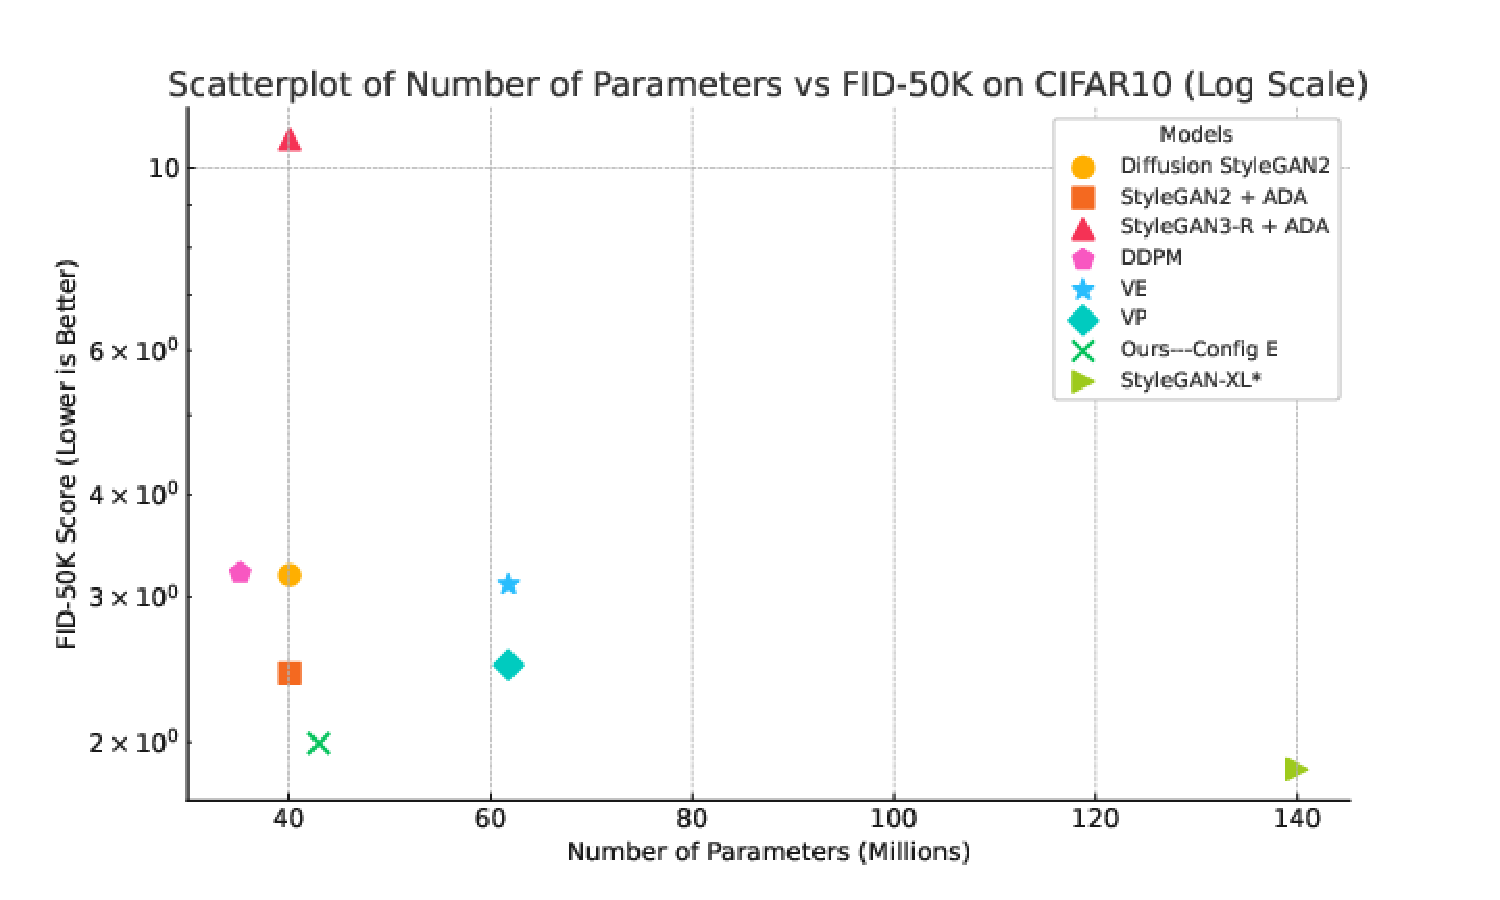
\includegraphics[width=\linewidth,clip,trim={0 0 0 2cm}]{figures/Scatterplot-FID-Parameters-CIFAR10.pdf}
    \caption{Millions of parameters vs.~FID-50K (log scale) on CIFAR-10. Lower is better.}
    \label{fig:fid-50k-vs-params-cifar-10}
\end{wrapfigure}

Many state-of-the-art GANs are derived from Projected GAN~\cite{sauer2021projected}, including StyleGAN-XL~\cite{sgxl} and the concurrent work of StyleSAN-XL~\cite{takida2024san}. These methods use a pre-trained ImageNet classifier in the discriminator. Prior work has shown that a pre-trained ImageNet discriminator can leak ImageNet features into the model~\cite{kynkaanniemi2022role}, causing the model to perform better when evaluating on FID since it relies on a pre-trained ImageNet classifier for the loss. But, this does not improve results in perceptual studies~\cite{kynkaanniemi2022role}. Our model produces its low FID without any ImageNet pre-training.

%\jt{Missing citations here for such methods.}


%\aaron{add NFEs}
%\jt{Which models in our evaluation use this? Any?}

%\jt{What is the second caveat?}

\subsection{FID --- ImageNet-32~\cite{chrabaszcz2017downsampled}}
\label{sec:imagenet32-fid-explain}
We train Config E model until convergence and with optimized hyperparameters and training schedule on ImageNet-32 (conditional generation). We compare against recent GAN models and recent diffusion models in Table~\ref{tab:imagenet32}.
We adjust the number of parameters in the generator of our model to match StyleGAN-XL~\cite{sgxl}'s generator (84M parameters). Specifically, we make the model significantly wider to match. Our method achieves comparable FID despite using a 60\% smaller discriminator (Tab.~\ref{tab:imagenet32}) and despite not using a pre-trained ImageNet classifier.
%, which has been shown to improve FID performance, but not improve results in perceptual studies~\cite{kynkaanniemi2022role}.

\vspace{-0.1cm}
\subsection{FID --- ImageNet-64~\cite{chrabaszcz2017downsampled}}
We evaluate our model on ImageNet-64 to test its scalability. We stack another resolution stage on our ImageNet-32 model, resulting in a generator of 104\ M parameters. This model is nearly 3$\times$ smaller than diffusion-like models~\cite{adm,edm,cm,icm} that rely on the ADM backbone, which contains about 300\ M parameters. Despite the smaller model size and that our model generates samples in one step, it outperforms larger diffusion models with many NFEs on FID (Tab.~\ref{tab:imagenet64}).

\vspace{-0.1cm}
\subsection{Recall}
We evaluate the recall~\cite{precrecall} of our model on each dataset to quantify sample diversity. In general, our model achieves a recall that is similar to or marginally worse than the diffusion model counterpart, yet superior to existing GAN models. For CIFAR-10, the recall of our model peaked at 0.57; as a point of comparison, StyleGAN-XL~\cite{sgxl} has a worse recall of 0.47 despite its lower FID. For FFHQ, we obtain a recall of 0.53 at 64$\times$64 and 0.49 at 256$\times$256, whereas StyleGAN2~\cite{sg2} achieved a recall of 0.43 on FFHQ-256. Our ImageNet-32 model achieved a recall of 0.63; comparable to ADM~\cite{adm}. Our ImageNet-64 model achieved recall 0.59. While this is slightly worse than $\approx$0.63 that many diffusion models achieve, it is better than BigGAN-deep~\cite{biggan} which achieved a recall of 0.48.

\begin{figure}
    \begin{floatrow}
        \capbtabbox{%
        \centering
        \resizebox{0.9\linewidth}{!}{
        \begin{tblr}{
          column{2} = {r},
          column{3} = {r},
          cell{8}{1} = {c=3}{},
          hline{2,7-8} = {-}{},
        }
    Model                                                       & NFE$\downarrow$  & FID$\downarrow$                        \\ 
    DDPM++~\cite{kim2021soft}                  & 1000 & 8.42                                   \\
    VDM~\cite{kingma2021variational}           & 1000 & 7.41                                   \\
    MSGAN~\cite{karnewar2020msg,ning2023input} & 1    & 12.3                                   \\
    ADM~\cite{adm}                             & 1000 & 3.60                                   \\
    DDPM-IP~\cite{ning2023input}               & 1000 & 2.87                                   \\
    Ours—Config E               & 1    & 1.27   \\
    \textit{With ImageNet feature leakage~\cite{kynkaanniemi2022role}:}    \\
    StyleGAN-XL*~\cite{sgxl}                   & 1    & 1.10                                  
    \end{tblr}
        }
    }{%
        \caption{\label{tab:imagenet32}ImageNet-32.}
        % \jt{some are conditional still}}
    }
    %
    \capbtabbox{
        \centering
        \resizebox{0.9\linewidth}{!}{
        \begin{tblr}{
          column{2} = {r},
          column{3} = {r},
          cell{1}{2} = {c},
          cell{1}{3} = {c},
          cell{12}{1} = {c=3}{},
          hline{2-3,11-12} = {-}{},
        }
        Model         & NFE$\downarrow$ & FID$\downarrow$ \\
        BigGAN-deep~\cite{biggan}\phantom{xx}   & 1               & 4.06            \\
        DDPM~\cite{ddpm}          & 250             & 11.0            \\
        DDIM~\cite{ddim}          & 50              & 13.7            \\
        ADM~\cite{adm}           & $^\S$250             & 2.91            \\
        EDM~\cite{edm}           & 79              & 2.23            \\
        CT~\cite{cm}            & 2               & 11.1            \\
        CD~\cite{cm}            & 3               & 4.32            \\
        iCT-deep~\cite{icm}      & 2               & 2.77            \\
        DMD~\cite{dmd}           & 1               & 2.62            \\
        Ours—Config E & 1               & 2.09            \\
        \emph{With ImageNet feature leakage~\cite{kynkaanniemi2022role}:}          &                 &                 \\
        StyleGAN-XL*~\cite{sgxl}   & 1               & 1.52            
        \end{tblr}
        }
    }
    {
        \caption{\label{tab:imagenet64}ImageNet-64.\hspace{-0.1cm} {\small \S:\hspace{-0.05cm}deterministic sampling.}}
    }
    \end{floatrow}
    \vspace{-0.25cm}
\end{figure}


% \begin{table}[ht]
%     \centering
%     \begin{tabular}{lcccccccc}
%         \toprule
%         \textbf{Model} & \textbf{\# Param.} & \textbf{IS $\uparrow$} & \textbf{FID $\downarrow$} & \textbf{Precision $\uparrow$} & \textbf{Recall $\uparrow$} & \textbf{Density $\uparrow$} & \textbf{Coverage $\uparrow$} & \textbf{Inf. (s)} \\
%         \midrule
%         ReACGAN + DiffAug (Ours) [10] & 9.4M & 10.15 & 2.64 & 0.75 & 0.65 & 0.98 & 0.90 & 0.009 \\
%         StyleGAN2-ADA [85] & 20.2M & 10.31 & 2.41 & 0.74 & 0.68 & 1.02 & 0.92 & 0.008 \\
%         StyleGAN2-ADA (Ours) [85] & 20.2M & \textbf{10.53} & 2.31 & 0.75 & 0.69 & 1.04 & 0.93 & 0.008 \\
%         StyleGAN2 + DiffAug + D2D-CE (Ours) [10] & 20.2M & 10.46 & 2.30 & 0.76 & 0.68 & 1.03 & 0.93 & 0.007 \\
%         DDPM [43] & 35.2M & 9.73 & 3.23 & 0.78 & 0.67 & 1.10 & 0.93 & 15.422 \\
%         DDPM++ [44] & 106.6M & 9.90 & 2.49 & 0.78 & 0.69 & 1.12 & 0.94 & 46.697 \\
%         NCSN++ [44] & 107.6M & 10.08 & 2.27 & 0.77 & 0.70 & 1.07 & 0.94 & 99.304 \\
%         LSGM [45] & - & 10.04 & 2.80 & 0.80 & 0.70 & 1.15 & 0.95 & - \\
%         LSGM-ODE [45] & - & 10.07 & \textbf{2.09} & 0.77 & 0.71 & 1.03 & 0.94 & - \\
%         CLD-SGM [47] & - & 9.88 & 2.38 & 0.78 & 0.69 & 1.12 & 0.94 & - \\
%         StyleGAN-XL~ & 18.0M & \textbf{11.03} & \textbf{1.88} & 0.77 & 0.59 & 1.08 & 0.94 & 0.010 \\
%         % BaselineGAN & %10.284011840820312
%         % 10.28
%         % & %1.9925376117527978 
%         % 1.99 & % 0.6899600028991699 
%         % 0.69 &&
%         \bottomrule
%     \end{tabular}
%     \caption{Comparison of various models on CIFAR10 dataset. TODO fix citation}
% \label{tab:cifar10_comparison}
%\end{table}

% \jt{Is the below meant to be a conclusion? Some of these statements are unfounded in the evidence we present so far.}
% \begin{enumerate}

%     \item We demonstrate the ability of our method to recover all modes of training data on Stacked Mnist~\ref{tab:stackedmnist}.
%     \item We beat all methods that do not use bCR (shown to overfit for FFHQ-256~\cite{}) and methods that do not leak imagenet features from a pretrained discriminator~\cite{kynkaanniemi2022role}. If we exclude these two categories of models, we are SOTA across all open source GANs. We also SOTA on a per parameter count basis on multiple GANs.
%     \item We demonstrate SOTA performance on CIFAR-10 image generation at our current parameter count, outperforming all previous GANs except for StyleGAN-XL derived ones with X\% percent of the parameters of these methods. We also do not leak features from ImageNet or use a pretrained discriminator.~\ref{tab:cifar10}. 
%     \item We achieve near SOTA on FFHQ 256 and achieve SOTA for a GAN method without bCR or feature leakage.
%     \item We achieve near state of the art results on Imagenet and achieve Pareto frontier results for total GAN model parameter size.
% \end{enumerate}
% \begin{table}[h]
\centering
\caption{FID on ImageNet-32}
\begin{tabular}{ l c c }
\toprule
Model & \textbf{Year} & FID$\downarrow$ \\
\midrule
% %Real NVP (Dinh et al.) & 2016 & 4.28 \\
% %Glow (Kingma and Dhariwal) & 2018 & 4.09 \\
% %MintNet & 2019 & 4.06 \\
% % Residual Flow & 2019 & 4.01 \\
% % BIVA Maaloe et al. & 2019 & 3.96 \\
% % ANF Huang et al. & 2020 & 3.92 \\
% % NVAE w/ flow & 2020 & 3.92 \\
% % PixelRNN & 2016 & 3.86 \\
% % Flow++ & 2019 & 3.86 \\
% % SPN Menick and Kalchbrenner & 2018 & 3.85 \\
% % Gated PixelCNN & 2016 & 3.83 \\
% % Very Deep VAE & 2020 & 3.8 \\
% % MRCNF & 2021 & 3.77 \\
% % $\delta$-VAE & 2019 & 3.77 \\
% Image Transformer~\cite{parmar2018image} & 2018 & 3.77 \\
% ScoreFlow & 2021 & 3.76 \\
% Reflected Diffusion & 2023 & 3.74 \\
% %Hourglass & 2021 & 3.74 \\
% DenseFlow-74-10 & 2021 & 3.63 \\
% i-DODE & 2023 & 3.43 \\
% MSGAN~\cite{karnewar2020msg} & 2019 & 12.3 \\
% DDPM-IP & 2023 & 2.66 \\
MSGAN~\cite{karnewar2020msg} & 2019 & 12.3 \\
VDM~\cite{kingma2021variational} & 2021 & 7.41 \\
DDPM++~\cite{kim2021soft} & 2021 & 8.42 \\
DDPM-IP~\cite{ning2023input} & 2023 & 2.87 \\
\textbf{Ours} & 2024 & 1.28 \\
StyleGAN-XL~\cite{sauer2022stylegan} & 2022 & \textbf{1.10} \\
\bottomrule
\end{tabular}
\end{table}

% \begin{table}[tO]
%     \centering
%     \begin{tabular}{c|c|c|c}
%          & FID\_50k & Precision & Recall \\
%         StyleGAN &  \\
%         StyleGAN-XL? &
%         Lots of other baselines
%     \end{tabular}
%     \caption{Caption}
%     \label{tab:my_label}
% \end{table}
% \label{sec:exp}
% % cifar10, ffhq, imagenet

% \begin{table}
%     \centering
%     %\caption{Results for CIFAR-10 generation. \aaron{add NFEs}}
%     %\vspace{-2mm}
%     \begin{tblr}{
%       column{2} = {r},
%       cell{1}{2} = {c},
%       hline{2,9,13} = {-}{},
%     }
%     Model               & FID$\downarrow$           \\
%     BigGAN~\cite{biggan}              & 14.73         \\
%     TransGAN~\cite{trans}            & 9.26          \\
%     ViTGAN~\cite{vitgan}              & 6.66          \\
%     DDGAN~\cite{ddgan}               & 3.75          \\
%     Diffusion StyleGAN2 & 3.19          \\
%     StyleGAN2 + ADA     & 2.42          \\
%     StyleGAN3-R + ADA   & 10.83         \\
%     DDPM                & 3.21          \\
%     DDIM                & 4.67          \\
%     VE                  & 3.11          \\
%     VP                  & 2.48          \\
%     Ours---Config E     & \textbf{1.99} 
%     \end{tblr}
%     %\label{tab:cifar10}
%     \caption{Results for CIFAR-10 generation. \aaron{add NFEs}}
%     \label{tab:cifar10}
% \end{table}



%%%%%%%%%%%%%%%%%%%%%%%%%%%%%%%%%%%%%%%%%%%%%%%%%%%%%%%%%%%%%
% Qualitative figures
%%%%%%%%%%%%%%%%%%%%%%%%%%%%%%%%%%%%%%%%%%%%%%%%%%%%%%%%%%%%%

% Variable to control the size of each image
% \begin{figure}
%     \centering
%     \includegraphics{example-image-a}
%     \caption{stacked mnist (qualitative figure) (from powerpoint)}
%     \label{fig:stacked-mnist}
% \end{figure}
% cifar10, ffhq, imagenet

% \noindent\begin{minipage}{.33\textwidth}
% \centering
% \captionof{table}{1000-mode coverage on StackedMNIST.}
% \vspace{-2mm}
% \begin{tblr}{
%   cell{2}{2} = {c},
%   cell{2}{3} = {c},
%   cell{3}{2} = {c},
%   cell{3}{3} = {c},
%   cell{4}{2} = {c},
%   cell{4}{3} = {c},
%   cell{5}{2} = {c},
%   cell{5}{3} = {c},
%   cell{6}{2} = {c},
%   cell{6}{3} = {c},
%   cell{7}{2} = {c},
%   cell{7}{3} = {c},
%   cell{8}{2} = {c},
%   cell{8}{3} = {c},
%   cell{9}{2} = {c},
%   cell{9}{3} = {c},
%   cell{10}{2} = {c},
%   cell{10}{3} = {c},
%   cell{11}{2} = {c},
%   cell{11}{3} = {c},
%   hline{2,11} = {1-3}{},
% }
% Model     & Modes$\uparrow$ & KLD$\downarrow$            &  \\
% DCGAN     & 99            & 3.40\phantom{0}&  \\f
% VEEGAN    & 150           & 2.95\phantom{0}&  \\
% WGAN-GP   & 959           & 0.73\phantom{0}&  \\
% PacGAN    & 992           & 0.28\phantom{0}&  \\
% StyleGAN2 & 940           & 0.42\phantom{0}&  \\
% PresGAN   & \textbf{1000} & 0.12\phantom{0}&  \\
% Adv. DSM  & \textbf{1000} & 1.49\phantom{0}&  \\
% VAEBM     & \textbf{1000} & 0.087          &  \\
% DDGAN     & \textbf{1000} & 0.071          &  \\
% Ours      & \textbf{1000} & \textbf{???} &  
% \end{tblr}
% \label{tab:stackedmnist}
% \end{minipage}%
% \begin{minipage}{.33\textwidth}
% \centering
% \captionof{table}{Results for CIFAR-10 generation.}
% \vspace{-2mm}
% \begin{tblr}{
%   column{2} = {r},
%   cell{1}{2} = {c},
%   hline{2,9,13} = {-}{},
% }
% Model               & FID$\downarrow$           \\
% BigGAN              & 14.73         \\
% TransGAN            & 9.26          \\
% ViTGAN              & 6.66          \\
% DDGAN               & 3.75          \\
% Diffusion StyleGAN2 & 3.19          \\
% StyleGAN2 + ADA     & 2.42          \\
% StyleGAN3-R + ADA   & 10.83         \\
% DDPM                & 3.21          \\
% DDIM                & 4.67          \\
% VE                  & 3.11          \\
% VP                  & 2.48          \\
% Ours                & \textbf{1.99} 
% \end{tblr}
% \label{tab:cifar10}
% \end{minipage}%
% \begin{minipage}{.33\textwidth}
% \centering
% \captionof{table}{Results on FFHQ ($256\times256$).}
% \vspace{-2mm}
% \begin{tblr}{
%   column{2} = {r},
%   cell{1}{2} = {c},
%   hline{2,5} = {-}{},
%   hline{2,9} = {-}{},
% }
% Model       & FID$\downarrow$  \\
% StyleGAN2   & 3.78 \\
% StyleGAN3-T & 4.81 \\
% StyleGAN3-R & 3.92 \\
% LDM & 4.98\\
% ADM (DDIM) & 8.41\\
% ADM (DPM-Solver) & 8.40\\
% Diffusion Autoencoder & 5.81\\
% Ours        & \textbf{2.95} 
% \end{tblr}
% \label{tab:ffhq256}
% \end{minipage}


% \input{tables/cifar10}
% \input{tables/ffhq256}
% \input{tables/MNIST}
\begin{figure}[h!]
    \newlength{\imgsize}
    \setlength{\imgsize}{0.10\linewidth} % Adjust this value to change the size of the images
    
    % New command to include images from a specific directory
    \newcommand{\qualitativeimg}[1]{%
        \includegraphics[width=\imgsize]{figures/qualitative/ffhq-256-000139623/image-#1.jpg}%
    }
    
    \setlength{\tabcolsep}{0pt} % Remove spacing between columns
    \renewcommand{\arraystretch}{0} % Remove spacing between rows
    
    \centering
    \begin{tabular}{cccccccc} % Eight columns
        \qualitativeimg{64} & \qualitativeimg{65} & \qualitativeimg{66} & \qualitativeimg{67} & \qualitativeimg{128} & \qualitativeimg{69} & \qualitativeimg{70} & \qualitativeimg{71} \\
        \qualitativeimg{72} & \qualitativeimg{73} & \qualitativeimg{74} & \qualitativeimg{75} & \qualitativeimg{76} & \qualitativeimg{77} & \qualitativeimg{78} & \qualitativeimg{79} \\
        \qualitativeimg{80} & \qualitativeimg{81} & \qualitativeimg{82} & \qualitativeimg{83} & \qualitativeimg{84} & \qualitativeimg{85} & \qualitativeimg{86} & \qualitativeimg{87} \\
        \qualitativeimg{88} & \qualitativeimg{89} & \qualitativeimg{90} & \qualitativeimg{91} & \qualitativeimg{92} & \qualitativeimg{93} & \qualitativeimg{94} & \qualitativeimg{95} \\
        \qualitativeimg{96} & \qualitativeimg{97} & \qualitativeimg{98} & \qualitativeimg{99} & \qualitativeimg{100} & \qualitativeimg{101} & \qualitativeimg{102} & \qualitativeimg{103} \\
        \qualitativeimg{104} & \qualitativeimg{105} & \qualitativeimg{106} & \qualitativeimg{107} & \qualitativeimg{108} & \qualitativeimg{109} & \qualitativeimg{110} & \qualitativeimg{111} \\
        \qualitativeimg{112} & \qualitativeimg{113} & \qualitativeimg{114} & \qualitativeimg{115} & \qualitativeimg{116} & \qualitativeimg{117} & \qualitativeimg{118} & \qualitativeimg{119} \\
        \qualitativeimg{120} & \qualitativeimg{121} & \qualitativeimg{122} & \qualitativeimg{123} & \qualitativeimg{124} & \qualitativeimg{125} & \qualitativeimg{126} & \qualitativeimg{127} \\
    \end{tabular}
    \caption{Qualitative examples of sample generation from our Config E on FFHQ-256.}
    \label{fig:ffhq-256-teaser}
\end{figure}


\section{Conclusion}
\label{sec:conclusion}
This paper introduced \tool, a language to describe distributed machine learning workloads and optimize them across computation and communication boundary. 
We show that \tool{} generated code significantly improves several training and inference times of large language models. 
In the future we plan to automate the optimizations through smart search.

% With ever increasing larger models being trained on massively
% distributed clusters using large datasets, there is a need for
% optimized communication and computation kernels.  Existing techniques
% to improve data-parallel and model-parallel training are limited to a
% particular algorithm, which might not be optimal for different input
% tensor sizes, topology of a distributed system.  In this paper, we
% presented \tool DSL to express programs that contains communication
% and computation and several transformations to optimize these programs
% for wide range of scenarios.  Code generated by \tool performs
% significantly better than hand-optimized state-of-the-arts.


\section*{Acknowledgments}

We thank Laurel Orr, Xun Huang, Trevor Gale, Jian Zhang, Victor Bittorf, Sarah Hooper, Neel Guha, and Michael Zhang for their helpful discussions and feedback on early drafts of the paper.

We gratefully acknowledge the support of NIH under No.\ U54EB020405 (Mobilize), NSF under Nos.\ CCF1763315 (Beyond Sparsity), CCF1563078 (Volume to Velocity), and 1937301 (RTML); ARL under No.\ W911NF-21-2-0251 (Interactive Human-AI Teaming); ONR under No.\ N000141712266 (Unifying Weak Supervision); ONR N00014-20-1-2480: Understanding and Applying Non-Euclidean Geometry in Machine Learning; N000142012275 (NEPTUNE); NXP, Xilinx, LETI-CEA, Intel, IBM, Microsoft, NEC, Toshiba, TSMC, ARM, Hitachi, BASF, Accenture, Ericsson, Qualcomm, Analog Devices, Google Cloud, Salesforce, Total, the HAI-GCP Cloud Credits for Research program,  the Stanford Data Science Initiative (SDSI), and members of the Stanford DAWN project: Facebook, Google, and VMWare. The U.S.\ Government is authorized to reproduce and distribute reprints for Governmental purposes notwithstanding any copyright notation thereon. Any opinions, findings, and conclusions or recommendations expressed in this material are those of the authors and do not necessarily reflect the views, policies, or endorsements, either expressed or implied, of NIH, ONR, or the U.S.\ Government.

\bibliography{ref}
\bibliographystyle{icml2022}


\newpage
\appendix
\onecolumn

\section{Extended Related Work}
\label{app:related}
In this section, we extend the related works referenced in the main paper and discuss them in detail.
\paragraph{Sparse Training.} Our work is loosely related to neural network pruning. By iteratively eliminating neurons and connections, pruning has seen great success in compressing complex models. \citet{han2015deep,han2015learning} put forth two naive but effective algorithms to compress models up to 49x and maintain comparable accuracy. \citet{li2016pruning} employ filter pruning to reduce the cost of running convolution models up to 38 $\%$, \citet{NIPS2017_a51fb975} prunes the network at runtime, hence retaining the flexibility of the full model. \citet{dong2017learning} prunes the network locally in a layer by layer manner.  \citet{sanh2020movement} prunes with deterministic first-order information, which is more adaptive to pretrained model weights. \citet{lagunas2021block} prunes transformers models with block sparsity pattern during fine-tuning, which leads to real hardware speed up while maintaining the accuracy. \citet{zhu2017prune} finds large pruned sparse network consistently outperform the small dense networks with the same compute and memory footprints. Although both our and all the pruning methods are aiming to produce sparse models, we differ in our emphasis on the overall efficiency, whereas pruning mostly focuses on inference efficiency and disregards the cost in finding the smaller model.

There has been more recent work on sparse methods that focuses on speeding up
training and not just inference, such as SNFS~\citep{dettmers2019sparse},
RigL~\citep{dettmers2019sparse}, Top-KAST~\citep{jayakumar2021top}.
These methods often focus on FLOP counts, which may not correlate well with
wall-clock time on modern hardware (e.g., GPUs).
Block-sparsity is another approach that exploits the block-oriented nature of
GPUs~\citep{gray2017gpu, child2019generating, guo2020accelerating}.
Sparse models have also been found useful to improve the training process of
dense models.
For example, sparsity can be used to regularize dense models to improve
accuracy~\citep{han2016dsd}, or to alternate between sparse and dense training
to ease deployment~\citep{peste2021ac}.
Our sparse-to-dense reverse sparsification instead focuses on speeding up dense
training, where the sparse model is used for efficiency and not regularization.


In addition, models proposed in our work can be roughly seen as a class of manually constructed lottery tickets. Lottery tickets \citet{frankle2018lottery} are a set of small sub-networks derived from a larger dense network, which outperforms their parent networks in convergence speed and potentially in generalization. A huge number of studies are carried out to analyze these tickets both empirically and theoretically: \citet{morcos2019one} proposed to use one generalized lottery tickets for all vision benchmarks and got comparable results with the specialized lottery tickets; \citet{frankle2019stabilizing} improves the stability of the lottery tickets by iterative pruning; \citet{frankle2020linear} found that subnetworks reach full accuracy only if they are stable against SGD noise during training; \citet{orseau2020logarithmic} provides a logarithmic upper bound for the number of parameters it takes for the optimal sub-networks to exist; \citet{pensia2020optimal} suggests a way to construct the lottery ticket by solving the subset sum problem and it's a proof by construction for the strong lottery ticket hypothesis. Furthermore, follow-up works \citep{liu2020finding, wang2020picking, tanaka2020pruning} show that we can find tickets without any training labels.


\paragraph{Structured matrices and butterfly matrices.}
Structured matrices are those with asymptotically fast matrix-vector
multiplication algorithm ($o(n^2)$ time complexity) and few parameters ($o(n^2)$
space complexity).
Common examples include sparse \& low-rank matrices, and fast transforms such as
Fourier transform, Chebyshev transform, Legendre transform, and more generally
orthogonal polynomial transforms.
These transforms have been widely used in data preprocessing (e.g., DFT in
speech processing~\citep{jurafsky2014speech}) and kernel
approximation~\citep{le2013fastfood,yu2016orthogonal}.
Many generalizations of these transforms have been used in machine learning to
replace dense weight
matrices~\citep{sindhwani2015structured,thomas2018learning,gu2020hippo}.
\citet{desa2018two} shows that any structured matrix (in the form of arithmetic
circuits) can be written as product of sparse matrices,
and~\citet{dao2020kaleidoscope} shows that products of butterfly matrices can
represent these structured matrices almost optimally in terms of runtime and
memory.
The class of butterfly matrices~\citep{parker1995random} have also been used in
kernel models~\citep{munkhoeva2018quadrature, choromanski2019unifying} and deep
learning models~\citep{vahid2020butterfly,lin2021deformable,
  ailon2021sparse}.

\paragraph{Neural Operators for PDEs.}

Deep learning has found application in the domain of differential equations and scientific computing \cite{rackauckas2020universal}, with methods developed for prediction and control problems \cite{kidger2020neural,massaroli2021differentiable}, as well as acceleration of numerical schemes \cite{poli2020hypersolvers,jolicoeur2021gotta}. Specific to the \textit{partial differential equations} (PDEs) are approaches designed to learn solution operators \cite{raissi2019physics,fan2020solving,li2020fourier}, and hybridized solvers \cite{kochkov2021machine}, evaluated primarily on classical fluid dynamics.

The promise of these approaches is to offer, at the cost of an initial training procedure, accurate yet faster solutions than an appropriate numerical method tuned for a specific problem, which can then be leveraged for real-time forecasting or within larger feedback loops. Nonetheless, optimal design of neural operators remains an open problem, with most relying on fast Fourier transforms (FFT) or standard dense neural architectures. Instead, neural operators based on Monarch are capable of approximating all fast transforms, thus allowing automated optimization towards a suitable transform on a given PDE problem.

\paragraph{MRI.} Accelerated multi-coil MRI is an essential mechanism for reducing long scan times and making certain scan types feasible. In multi-coil MRI, data is acquired in the spatial Fourier domain (a.k.a \textit{k-space}) across multiple coils (sensors). To reduce scan time, this data is sampled below the required rate for recovering the underlying signal (i.e. Nyquist rate), which results in signal aliasing (see Appendix \ref{sec:experiment_details_mri}). In these settings, direct application of the inverse fast Fourier transform (FFT) cannot suppress aliasing artifacts.

Classical MRI reconstruction approaches supplement the FFT by leveraging shared information across multiple coils and strong analytical priors to regularize image recovery objectives. SENSE-based methods jointly dealias images across multiple coils and reweight the final image based on the spatial sensitivity profile of each coil \citep{pruessmann1999sense}. Compressed sensing promotes image sparsity in transformation domains (e.g. Fourier, wavelet) while enforcing data consistency between the Fourier transform of the reconstructed image and the observed measurements \citep{lustig2007sparse}. Low-rank methods enforce low rank structure across slowly-varying dimensions or local patches in the data \citep{ong2016beyond,ravishankar2017low,haldar2013low}. Additionally, GRAPPA-based techniques optimize kernels to directly interpolate missing k-space samples to promote smoothness in the Fourier domain \cite{griswold2002generalized}. Despite their efficacy, these methods have long reconstruction times, require explicit analytical priors, and require careful hyperparameter fine-tuning.

CNNs have shown promise as a fast-at-inference, learnable alternative to classical MRI reconstruction methods \cite{knoll2020deep}. In supervised learning, fully convolutional networks (e.g. U-Net \citep{ronneberger2015u} or unrolled networks \citep{sandino2020compressed,hammernik2018learning}) learn a mapping between paired zero-filled and fully-sampled, ground truth images. However, supervised methods require a large fully-sampled (labeled) data corpus and are sensitive to distribution drifts due to patient, hardware, and sequence heterogeneity \cite{darestani2021measuring}. To reduce dependence on labeled data, unsupervised methods have used generative adversarial networks \citep{cole2020unsupervised, mardani2018deep}, self-supervised learning \cite{yaman2020self}, dictionary learning \cite{lahiri2021blind}, and untrained networks \cite{darestani2021accelerated}. Despite their 
label efficiency, these techniques still underperform supervised methods and are also sensitive to distribution shift. Recently, a family of semi-supervised reconstruction methods demonstrated label efficiency and robustness to physics-driven perturbations, such as changes in signal-to-noise ratio or patient motion \citep{desai2021noise2recon, desai2021vortex}. However, these methods require large amounts of unlabeled data, which can be difficult to curate in few-shot settings. Thus, despite their success in controlled environments, prospective clinical deployment of these models has been stifled \citep{chaudhari2020prospective}.

In our work, we propose a model with a single FFT-initialized factorized Monarch matrix. Such a matrix can provide the benefits of both a simple linearized transformation like FFT and a learnable mechanism to remove aliasing artifacts resulting from the undersampled k-space. The smaller learnable parameter set may reduce overfitting in data-limited settings while preserving the transformation structure of Fourier matrices. Thus, our approach can be interpreted as a hybrid between analytically-constrained classical methods and data-dependent CNNs.


\section{Notation Review}
Throughout this paper, we use lowercase to denote scalars (e.g., $k$), lowercase boldface to denote vectors (e.g., $\vv$), and uppercase boldface to denote matrices (e.g., $\vA$).

$\vI$ denotes the identity matrix. We use $\vA^\top$ to denote the transpose of a matrix and $\vA^*$ to denote the conjugate transpose of a matrix. All results in this paper apply to matrices over the either the reals $\mathbb{R}$ or the complex numbers $\mathbb{C}$; when the field under consideration can be either one of these, we denote it by $\mathbb{F}$.

We use 1-indexing throughout this paper except where explicitly stated.


\newcommand{\baseb}[3]{\parens{{#1},{#2}}_{{#3}}}
\newcommand{\mx}[1]{\mathbf{#1}}
\newcommand{\floors}[1]{\left \lfloor #1 \right \rfloor}
\newcommand{\parens}[1]{\left( {#1}\right)}

\section{General Monarch Matrix Parametrization}
\label{sec:permutation}

In Section \ref{sec:Monarch_square}, we define a parametrization for square Monarch matrices of different ``block sizes'' (i.e., not necessarily $\sqrt{n}$), and prove some basic properties about them. In Section \ref{sec:Monarch_rect}, we further extend this to define rectangular Monarch matrices, and prove some basic properties about them.

Note: In this section, we use 0-indexing rather than 1-indexing, for notational convenience.

\subsection{General square matrices}
\label{sec:Monarch_square}
\subsubsection{Parametrization}
\label{sec:Monarch_square_param}
In this section, we define a more general Monarch parametrization for square matrices, allowing for different ``block sizes.'' Like \cref{def:Monarch}, the parametrization involves the product of a permuted block-diagonal matrix with another block-diagonal matrix; the difference is that we now allow the matrices $\vL$ and $\vR$ to have diagonal blocks of different sizes. Thus, the permutations applied to $\vL$ (to turn it into a block matrix where each block matrix is diagonal) will correspondingly also be different.

First, in \cref{def:square_r}, we define notation for a class of block-diagonal matrices.

\begin{definition}[Class $\BD\ind{b, n}$]
\label{def:square_r}
Let $b \in (1, n)$ be an integer that divides $n$. For $0\le i< \frac {n}{b}$, let $\mx{R}_{i}\in\F^{b \times b }$ be a $b \times b $ ``block" matrix. Then define the matrix $\vR$ with {\em block size} $b$ as follows:
\begin{equation}
 \label{eq:def-R}
  \vR = \diag\left(\vR_0, \dots, \vR_{\frac {n}{b}-1}\right).
\end{equation}
\end{definition}
(Note that the number of possible nonzero values in $\vR$ is $\frac {n}{b}\cdot b^2=nb$.)
We denote the class of all matrices $\vR$ expressible in this form by $\BD\ind{b, n}$. Note that this class is closed under (conjugate) transposition and contains the identity matrix.

Next, in \cref{def:Matrix L}, we define notation for a class of block matrices whose \emph{blocks} are diagonal.

\begin{definition}[Class $\DB\ind{b,n}$]
\label{def:Matrix L}
Let $b \in (1, n)$ be an integer that divides $n$. For $0 \le i, j < b$, let $\mx{D}_{i,j}\in\F^{b\times b}$ be a $b \times b$ diagonal matrix.
Then let $\vL$ be an $n \times n$ matrix with the following form: 
    \begin{equation}
        	\label{eq:def-L}
    \vL=
    	\begin{bmatrix}
    		\mx{D}_{0,0} & \dots & \mx{D}_{0,\frac{n}{b} -1} \\
    		\vdots & \ddots & \vdots \\
    		\mx{D}_{\frac{n}{b} -1,0} & \dots & \mx{D}_{\frac{n}{b} -1,\frac{n}{b} -1}
    	\end{bmatrix}
    \end{equation}
\end{definition}
(Note that the number of possible nonzero values in $\vL$ is $\parens{\frac nb}^2\cdot b=\frac{n^2}b$.)
We denote the class of all matrices $\vL$ expressible in this form by $\DB\ind{b, n}$. Note that this class is closed under (conjugate) transposition and contains the identity matrix. As we show in \cref{sec:sq-Monarch-properties}, $\vL$ can be written as a block-diagonal matrix with $b$ blocks of size $\ff{n}{b} \times \ff{n}{b}$ (i.e., a matrix in $\BD\ind{\frac{n}{b}, \, n}$), multiplied on the left and right with appropriate permutation matrices.
We denote the class of all matrices $\vL$ expressible in this form by $\DB\ind{b, n}$. Note that this class is closed under (conjugate) transposition. As we show in \cref{sec:sq-Monarch-properties}, $\vL$ can be written as a block-diagonal matrix with $b$ blocks of size $\ff{n}{b} \times \ff{n}{b}$ (i.e., a matrix in $\BD\ind{\frac{n}{b}, \, n}$), multiplied on the left and right with appropriate permutation matrices.

Using these two definitions, we define the class of Monarch matrices with a given block size.
\begin{definition}[Class $\M\ind{b,n}$]
\label{def:block_Monarch}
Let $b \in (1, n)$ be an integer that divides $n$. A \emph{Monarch matrix} of size $n \times n$ and ``block size $b$'' is a matrix of the form: 
    \begin{equation}
        	\label{eq:Monarch-general}
    \vM= \vL \vR
    \end{equation}
    where $\vL \in \DB\ind{b,n}$ and $\vR \in \BD\ind{b,n}$.
\end{definition}
We denote the class of all matrices $\vM$ expressible in this form by $\M\ind{b, n}$. Observe that when $b = \sqrt{n}$, this is exactly the matrix class $\M\ind{n}$ in \cref{def:Monarch}. (In other words, $\M\ind{n}$ is shorthand for $\M\ind{\sqrt{n}, n}$.) Note that a matrix in $\M\ind{b,n}$ is represented by $\frac{n^2}{b} + nb$ parameters.

We remark that $\M\ind{b,n} \supset \B\ind{n}$ for all block sizes $b \in (1, n)$ that divide $n$.

Based on \cref{def:block_Monarch}, we define the classes $\M\M^{*(b,n)}$ and $\M^*\M^{(b,n)}$::
\begin{definition}[Class $\M\M^{*(b,n)}$, $\M^*\M^{(b,n)}$]
\label{def:block_MM}
Let $b \in (1, n)$ be an integer that divides $n$ and suppose $\vM_1, \vM_2 \in \M^{(b,n)}$. We define $\M\M^{*(b,n)}$ to be the the class of all matrices $\vM$ expressible in the form $\vM= \vM_1 \vM_2^*$. \newline
We define $\M^*\M^{(b,n)}$ to be the the class of all matrices $\vM$ expressible in the form $\vM= \vM_1^* \vM_2$.
\end{definition}
Observe that when $b = \sqrt{n}$, $\M\M^{*(b,n)}$ is exactly the matrix class $\M\M^{*(n)}$ defined in \cref{sec:theory}. Note that a matrix in $\M\M^{*(b,n)}$ or $\M^*\M\ind{b,n}$. is represented by $2\frac{n^2}{b} + 2nb$ parameters.

Finally, we define the following ``Monarch hierarchy'' based on the kaleidoscope hierarchy of \cite{dao2020kaleidoscope}:
\begin{definition}[Class $(\M\M^{*(b,n)})^w_e$]
\label{def:block_MM}
Let $b \in (1, n)$ be an integer that divides $n$. We define the matrix class $(\M\M^{*(b,n)})^w_e$ as the set of all matrices $\vM$ that can be expressed as
    \begin{equation}
        	\label{eq:mm-hierarchy}
    \vM= \lt \pd{i=1}{w} \vM_i\rt [1:n, 1:n]
    \end{equation}
    where each $\vM_i \in \M\M^{*(b,e\cdot n)}$.
\end{definition}
Note that a matrix in $(\M\M^{*(b,n)})^w_e$ is represented by $2w\frac{e^2n^2}{b} + 2wenb$ parameters.

\subsubsection{Properties}
\label{sec:sq-Monarch-properties}
Here we show some properties of the matrix classes defined above. We first show some basic equivalent ways to define these classes. We then show (\cref{thm:lr_permutation}) that the matrices in $\DB\ind{b, n}$ are permuted block-diagonal matrices; specifically, that they can be converted to matrices in $\BD\ind{\frac{n}{b}, n}$ by applying the appropriate permutation. Finally, we state an expressivity result for the general ``Monarch hierarchy''  which follows from Theorem 1 of \cite{dao2020kaleidoscope}.

First, we define a class of permutations.
Let $1\le b\le n$ be integers such that $b$ divides $n$.
We will need to express each index $0\le i<n$ in ``block form.'' More specifically:

\begin{definition}\label{def:$i$}
Let $i \ge 0$, $b \ge 1$ be integers. Then define
\[i_0=i\mod{b},\]
and
\[i_1=\floors{\frac ib}.\] 
We use the notation $i\equiv\baseb{i_1}{i_0}{b}$ to denote the representation above. In particular, if $i\equiv(i_1,i_0)_{b}$,
then we have
\[
        i = i_1 \cdot b + i_0
\]
\end{definition}

Using this notation, we define the following class of permutations:
\begin{definition}
\label{def:sigma-b}
Let $b \in [1, n]$ be an integer that divides $n$.  Let $i\equiv\baseb{i_1}{i_0}{b}$. Define
    \begin{equation}
            \label{eq:sigma_b-def}
        \sigma_{(b,n)}(i) = i_0\cdot\frac{n}{b} + i_1.
    \end{equation}
That is, $\sigma_{(b,n)}(i)\equiv \baseb{i_0}{i_1}{\frac {n}{b}}$.
Let $\vP_{(b,n)}$ denote the $n \times n$ permutation matrix defined by the permutation $\sigma_{(b,n)}$.
\end{definition}
Intuitively, $\vP_{(b,n)}$ can be interpreted as reshaping a length-$n$ vector into an $b \times \ff{n}{b}$ matrix in row-major order, transposing the result, and then flattening this back into a vector (again in row-major order).


Now, we restate the formulation in \cref{def:square_r} equivalently as:
\begin{proposition}

\label{prop:R-eqv-def}
A matrix $\vR$ satisfies~\Cref{eq:def-R} (i.e., $\vR \in \BD\ind{b,n}$) if and only if the following holds for any
$0\le i,j< n$. Let $i\equiv\baseb{i_1}{i_0}{b}$ and $j\equiv\baseb{j_1}{j_0}{b}$.  Then
\begin{enumerate}
    \item\label{item:zero-loc-R} if $i_1\ne j_1$, then $\vR[i,j]=0$. 
    \item \label{item:nonzero-loc-R} Else (i.e., when $i_1=j_1$), then $\vR[i,j]=\vR_{i_1}[i_0,j_0]$.
\end{enumerate}

\end{proposition}



We restate the formulation in \cref{def:Matrix L} equivalently as:
\begin{proposition}
\label{prop:L-eqv-def}
A matrix $\vL$ satisfies~\Cref{eq:def-L} (i.e., $\vL \in \DB\ind{b,n}$) if and only if the following holds for any
$0\le i,j< n$. Let $i\equiv\baseb{i_1}{i_0}{b}$ and $j\equiv\baseb{j_1}{j_0}{b}$. Then 
\begin{enumerate}
    \item\label{item:zero-loc-L} if $i_0\ne j_0$, then $\vL[i,j]=0$. 
    \item \label{item:nonzero-loc-L} Else, (i.e., when $i_0=j_0$), then $\vL[i,j]=\vD_{i_1,j_1}[i_0,i_0]$.
\end{enumerate}
\end{proposition}

We will argue the following:
\begin{theorem}\label{thm:lr_permutation} Let $1\le b\le n$ such that $b$ divides $n$.
Recall that $\vP_{(b,n)}$ is the permutation matrix defined by the permutation $\sigma_{(b,n)}$. Let $\vL$ be a matrix in $\DB\ind{b, n}$. Then we have
\[\vR'=\vP_{(b,n)}\cdot\vL\cdot\vP_{(b,n)}^\top,\]
where $\vR' \in \BD\ind{\frac{n}{b},\, n}$.
\end{theorem}

\begin{proof}
We first note that multiplying an $n\times n$ matrix on the right (and left resp.) by $\vP_{(b,n)}^\top = \vP_{(\frac nb,n)}$ (and $\vP_{(b,n)}$ resp.) permutes the columns (and rows resp.) of the matrix according to $\sigma_{(b,n)}$.\footnote{This uses the fact that $\parens{\sigma_{(b,n)}}^{-1}=\sigma_{(\frac nb,n)}$ (which means $P_{(\frac{n}{b}, n)} = P_{(b, n)}^\top$ since the inverse of a permutation matrix is its transpose).} This implies that for any $0\le i,j<n$:
\begin{equation}
\label{eq:L-permuted}
\vR'[\sigma_{(b,n)}(i),\sigma_{(b,n)}(j)]=\vL[i,j].
\end{equation}
To complete the proof, we will argue that $\vR'$ satisfies the two conditions in~\Cref{prop:R-eqv-def}.

Towards this end, let $0\le i,j<n$ be arbitrary indices and further, define $i=\baseb{i_1}{i_0}{b}$ and $j=\baseb{j_1}{j_0}{b}$. Then note that $\sigma_{(b,n)}(i)=\baseb{i_0}{i_1}{\frac nb}$ and $\sigma_{(b,n)}(j)=\baseb{j_0}{j_1}{\frac nb}$.

By~\Cref{prop:L-eqv-def}, we have that if $i_0\ne j_0$, then $\vL[i,j]=0$. Note that $i_0\ne j_0$ satisfies the pre-condition for base size $\frac nb$ for indices $(\sigma_{(b,n)}(i),\sigma_{(b,n)}(j))$ in item~\ref{item:zero-loc-R} in~\Cref{prop:R-eqv-def}.  Then   by~\cref{eq:L-permuted}, we have that $\vR'[\sigma_{(b,n)}(i),\sigma_{(b,n)}(j)]=0$, which satisfies item~\ref{item:zero-loc-R} in~\Cref{prop:R-eqv-def}.

Now consider the case that $i_0=j_0$; then by item~\ref{item:nonzero-loc-L} in~\Cref{prop:L-eqv-def}, we have that $\vL[i,j]=\vD_{i_1,j_1}[i_0,i_0]$.  Note that $i_0= j_0$ satisfies the pre-condition for base size $\frac nb$ for indices $(\sigma_{(b,n)}(i),\sigma_{(b,n)}(j))$ in item~\ref{item:nonzero-loc-R} in~\Cref{prop:R-eqv-def} if we define $\vR'_{i_0}\in\F^{\frac nb\times\frac nb}$ as follows:
\[\vR'_{i_0}[i_1,j_1]=\vD_{i_1,j_1}[i_0,i_0].\] 
Note that the above implies that 
\[\vR'=\diag\parens{\vR'_0,\dots,\vR'_{b-1}},\]
where $\vR'_{\cdot}$ is as defined in the above paragraph. This means $\vR' \in \BD\ind{\frac{n}{b}, n}$, since each block $\vR_{i_0}'$ is a matrix of size $\frac{n}{b} \times \frac{n}{b}$.
\end{proof}

We now briefly note some alternate ways to express matrices in $\M\M^{*(b,n)}$.
\begin{proposition}
\label{prop:mm-eqv-def}
For any $\vM \in \M\M^{*(b,n)}$, we can write $\vM = (\vP_{(b,n)}^\top \vL_1 \vP_{(b,n)}) \vR (\vP_{(b,n)}^\top\vL_2\vP_{(b,n)})$, where $\vL_1,\vL_2 \in \BD\ind{\frac{n}{b},n}$ and $\vR \in \BD\ind{b,n}$.
\end{proposition}
\begin{proof}
By definition (see \cref{def:square_r} and \cref{def:Matrix L}), if $\vM \in \M\M^{*(b,n)}$, we can write
$\vM = (\vL_1' \vR_1) (\vL_2' \vR_2)^* = \vL_1' (\vR_1^* \vR_2) \vL_2'^*$,
where $\vL_1',\vL_2' \in \DB\ind{b,n},\vR_1,\vR_2 \in \BD\ind{b,n}$.

Notice that since $\vR_1^*, \vR_2$ are both block-diagonal with the same structure (i.e., both have blocks of size $b \times b$), their product $\vR$ is also in $\BD\ind{b,n}$.
Also, by \cref{thm:lr_permutation} we can write $\vL_1 = \vP_{(b,n)} \vL_1' \vP_{(b,n)}^\top$, $\vL_2 = \vP_{(b,n)} \vL_2' \vP_{(b,n)}^\top$, where $\vL_1,\vL_2$ are both in $\BD\ind{\frac{n}{b},n}$ (i.e., block diagonal with blocks of size $\frac{n}{b} \times \frac{n}{b}$).


Thus, we can write $\vM = (\vP_{(b,n)}^\top \vL_1 \vP_{(b,n)}) \vR (\vP_{(b,n)}^\top\vL_2\vP_{(b,n)})$, where $\vL_1,\vL_2 \in \BD\ind{\frac{n}{b},n}$ and $\vR \in \BD\ind{b,n}$.
\end{proof}

We use the above to show a simple relationship between $\M\M^{*(b,n)}$ and $\M^*\M^{(b,n)}$.
\begin{proposition}
\label{prop:mstarm}
If $\vM \in \M\M^{*(b,n)}$, then $\vP_{(b,n)} \vM \vP_{(b,n)}^\top \in \M^*\M\ind{\frac{n}{b},n}$. Conversely, if $\vM \in \M^*\M^{(b,n)}$, then $\vP_{(b,n)}^\top \vM \vP_{(b,n)} \in \M^*\M\ind{\frac{n}{b},n}$.
\end{proposition}
\begin{proof}
Suppose $\vM \in \M\M^{*(b,n)}$. By \cref{prop:mm-eqv-def} we can write $\vM = (\vP_{(b,n)}^\top \vL_1 \vP_{(b,n)}) \vR (\vP_{(b,n)}^\top\vL_2\vP_{(b,n)})$, where $\vL_1,\vL_2 \in \BD\ind{\frac{n}{b},n}$ and $\vR \in \BD\ind{b,n}$.
Thus $\vP_{(b,n)} \vM \vP_{(b,n)}^\top =
\vL_1 (\vP_{(b,n)} \vR \vP_{(b,n)}^\top) \vL_2$.

Letting $\vL_1' = \vL_1, \vL_2' = \vL_2^*, \vR_1' = \vP_{(b,n)} \vR \vP_{(b,n)}^\top$, and $\vR_2' = \vI$, we have $\vL_1', \vL_2' \in \BD\ind{\frac{n}{b}, n}$, $\vR_1', \vR_2' \in \DB\ind{\frac{n}{b}, n}$, and
$\vL_1 (\vP_{(b,n)} \vR \vP_{(b,n)}^\top) \vL_2 = 
\vL_1' \vR_1' \vR_2'^* \vL_2'^* = (\vL_1' \vR_1')(\vL_2' \vR_2')^* = \vM_1'\vM_2'^*$, where $\vM_1' = \vL_1' \vR_1', \vM_2' = \vL_2' \vR_2'$, so $\vM_1', \vM_2' \in \M^*\M\ind{\frac{n}{b},n}$.

Now instead suppose $\vM \in \M^*\M^{(b,n)}$. So $\vM = \vM_1^* \vM_2 = \vR_1^* \vL_1^* \vL_2 \vR_2$ for some $\vR_1, \vR_2 \in \BD\ind{b,n}$ and $\vL_1, \vL_2 \in \DB\ind{b,n}$. Thus by \cref{thm:lr_permutation} (and the fact that $\BD\ind{b,n}$ is closed under conjugate transposition) we can write $\vR_1^* = \vP_{(\frac{n}{b},n)}^\top \vR_1' \vP_{(\frac{n}{b}, n)} = \vP_{(b,n)} \vR_1' \vP_{(b, n)}^\top$ for some $\vR_1' \in \DB\ind{\frac{n}{b}, n}$, and similarly, can write $\vR_2 = \vP_{(b,n)} \vR_2' \vP_{(b,n)}^\top$ for some $\vR_2' \in \DB\ind{\frac{n}{b}, n}$. 

So $\vP_{(b,n)}^\top \vM \vP_{(b,n)} = \vR_1' (\vP_{(b, n)})^\top \vL_1^*)(\vL_2 \vP_{(b, n)})) \vR_2' =
 \vR_1' (\vP_{(b, n)}^\top \vL_1^* \vP_{(b, n)})(\vP_{(b, n)}^\top \vL_2 \vP_{(b, n)}) \vR_2' = (\vR_1' \vL_1')(\vL_2' \vR_2')$, where $\vL_1' = \vP_{(b, n)}^\top \vL_1^* \vP_{(b, n)}$, $\vL_2' = \vP_{(b, n)}^\top \vL_2 \vP_{(b, n)}$ are in $\BD\ind{\frac{n}{b}, n}$ by \cref{thm:lr_permutation}. Thus letting $\vM_1' = \vR_1'\vL_1'$, $\vM_2' = \vR_2^*\vL_2'^*$, we have $\vM = \vM_1' \vM_2'^*$ with $\vM_1', \vM_2' \in \M^{*(\frac{n}{b},n)}$.
\end{proof}

We now show that the class $\M\ind{b,n}$ strictly contains the class $\B\ind{n}$ of $n \times n$ butterfly matrices (as defined in \citet{dao2020kaleidoscope}). We first show two elementary ``helper'' results.

\begin{proposition}
\label{prop:bd-contain}
If $b,\, c \in (1, n)$ are such that $b$ divides $c$ and $c$ divides $n$, then $\BD\ind{b, n} \subseteq \BD\ind{c, n}$.
\end{proposition}
\begin{proof}
Suppose $\vR \in \BD\ind{b, n}$. Then by \cref{prop:R-eqv-def}, $\vR[i, j] = 0$ whenever $\floor{\frac{i}{b}} \ne \floor{\frac{j}{b}}$. Thus, whenever $\floor{\frac{i}{c}} \ne \floor{\frac{j}{c}}$, $\vR[i, j] = 0$, since $\floor{\frac{i}{c}} \ne \floor{\frac{j}{c}}$ implies $\floor{\frac{i}{b}} \ne \floor{\frac{j}{b}}$ by the assumption that $b$ divides $c$.
Applying \cref{prop:R-eqv-def} again, this means $\vR \in \BD\ind{c,n}$ as well.
\end{proof}

\begin{proposition}
\label{prop:db-contain}
If $b,\, c \in (1, n)$ are such that $b$ divides $c$ and $c$ divides $n$, then $\DB\ind{c, n} \subseteq \DB\ind{b, n}$.
\end{proposition}
\begin{proof}
Suppose $\vL \in \DB\ind{c, n}$. Then by \cref{prop:L-eqv-def}, $\vL[i, j] = 0$ whenever $(i \mod c) \ne (j \mod c)$. Thus, whenever $(i \mod b) \ne (j \mod b)$, $\vL[i, j] = 0$, since $(i \mod b) \ne (j \mod b)$ implies $(i \mod c) \ne (j \mod c)$ by the assumption that $b$ divides $c$.
Applying \cref{prop:L-eqv-def} again, this means $\vL \in \DB\ind{b,n}$ as well.
\end{proof}


\begin{theorem}
\label{thm:b_contained}
Let $n \ge 4$ be a power of 2. The class of matrices $\B\ind{n}$ is a subset of the class $\M\ind{b, n}$, for all $b \in (1, n)$ that divide $n$. When $n \ge 512$ it is a strict subset.
\end{theorem}
\begin{proof}
Recall from \cref{sec:butterfly} that if $\vB \in \B\ind{n}$, it has a \emph{butterfly factorization} 
$\vB = \vB_n \vB_{n/2} \hdots \vB_2$, where each $\vB_i \in \BF\ind{n, i}$.

Consider multiplying together the factors $\vB_b \vB_{b/2} \dots \vB_2$ (where $b \in (1, n)$ divides $n$). Since $\vB_i \in \BF\ind{n,i}$, by definition it is block diagonal with diagonal blocks of size $i \times i$; in other words, $\vB_i \in \BD\ind{i, n}$. Thus, each of the matrices $\vB_b, \vB_{b/2}, \dots, \vB_2$ is in $\BD\ind{b, n}$ (by \cref{prop:bd-contain}), i.e. block-diagonal with block size $b \times b$. This means their product $\vB_b \vB_{b/2} \dots \vB_2$ is also block diagonal with block size $b \times b$, i.e., it is in $\BD\ind{b, n}$.

Now, note that since $\vB_i \in \BF\ind{n,i}$, by definition it is a block matrix with blocks of size $i/2 \times i/2$, where each block is a diagonal matrix (note that some of these blocks are zero, except for the case of $\vB_n$). In other words, $\vB_i \in \DB\ind{i/2, n}$. Thus, for all $i \in \{n, n/2, \dots, 2b\}$, $\vB_i \in \DB\ind{(2b)/2, n} = \DB\ind{b, n}$ (by \cref{prop:db-contain}). So, their product $\vB_n \vB_{n/2} \dots \vB_{2b}$ is in $\DB\ind{b, n}$ as well, as by \cref{thm:lr_permutation} we can write $\vB_n \vB_{n/2} \dots \vB_{2b} = \vP_{(b,n)}^\top (\vP_{(b,n)} \vB_n \vP_{(b,n)}^\top) (\vP_{(b,n)} \vB_{n/2} \vP_{(b,n)}^\top) \dots (\vP_{(b,n)} \vB_{2b} \vP_{(b,n)}^\top) \vP_{(b,n)}$ and each of the $\vP_{(b,n)} \vB_i \vP_{(b,n)}^\top$'s in the preceding expression is in $\BD\ind{\frac{n}{b}, n}$.

Thus, if we let $\vL = \vB_n \vB_{n/2} \dots \vB_{2b}$ and $\vR = \vB_b \vB_{b/2} \dots \vB_2$,  we have $\vB = \vL\vR$ and $\vL \in \DB\ind{b, n}$, $\vR \in \BD\ind{b, n}$, which means that $\vB \in \M\ind{b,n}$ (\cref{def:block_Monarch}).

To show that the inclusion is strict, notice that any $\vM \in \M\ind{b,n}$ is the product of $\vL$ and $\vR$, where $\vR \in \BD\ind{b, n}$ and $\vP_{(b,n)}^\top \vL \vP_{(b,n)} \in \BD\ind{\frac{n}{b}, n}$ (by \cref{thm:lr_permutation}). Notice that the identity matrix is contained in both $\BD\ind{b,n}$ and $\DB\ind{b,n}$. Suppose first that $b \le \sqrt{n}$. Then even if we set $\vR$ to the identity, $\vM$ has at least $\frac{n^2}{b} \ge n^{3/2}$ free parameters (the entries in the blocks of the block-diagonal matrix $\vP_{(b,n)}^\top \vL \vP_{(b,n)}$ can be arbitrary, and there are $b$ such blocks each of size $\frac{n}{b}$). Similarly, in the case $b > \sqrt{n}$, we can set $\vL$ to the identity, and $\vM$ has at least $nb \ge n^{3/2}$ free parameters (the entries of the block-diagonal matrix $\vR$ can be arbitrary, and there are $nb$ total of these). Thus, at least $n^{3/2}$ parameters are required to uniquely describe any matrix in $\M\ind{b,n}$. However, a butterfly matrix in $\B\ind{n}$ has only $2n \log_2 n$ parameters. For $n > 256$, $2n \log_2 n < n^{3/2}$. (Note that this analysis is not tight: a more careful analysis can show the inclusion is strict even for smaller values of $n$.)

\end{proof}

We end this section with a theorem on the expressivity of the ``monarch hierarchy'' (products of monarch matrices), which follows from Theorem 1 of \cite{dao2020kaleidoscope}.
\begin{theorem}[Monarch hierarchy expressivity]
\label{thm:monarch_hierarchy}
Let $\vM$ be an $n \times n$ matrix such that matrix-vector multiplication of $\vM$ and an arbitrary vector $\vv$ (i.e., computation of $\vM \vv$) can
be represented as a linear arithmetic circuit with depth $d$ and $s$ total gates. Let $b \in (1, n)$ be a power of 2 that divides $n$.
Then, $\vM \in (\M\M^{*(b, n)})^{O(d)}_{O(s/n)}$.
\end{theorem}
\begin{proof}
Theorem 1 of \citet{dao2020kaleidoscope} says that if $n$ is a power of 2 and $\vA$ is an $n \times n$ matrix such that multiplying any vector $v$ by $\vA$ can be represented as a linear arithmetic circuit with depth $\le d$ and $\le s$ total gates, then $\vA \in (\B\B^{*(n)})^{O(d)}_{O(s/n)}$ (this is the ``kaleidoscope representation'' of $\vA$).

Recall from \cref{thm:b_contained} that for any $b \in (1, n)$ that is a power of 2 and divides $n$, $\M\ind{b, n} \supset \B\ind{n}$; thus, this implies $\M\M^{*(b,e\cdot n)} \supset \B\B^{*(e\cdot n)}$, and in turn $(\M\M^{*(b,n)})^w_e \supset (\B\B^{*(n)})^w_e$.

As $\vA \in  (\B\B^{*(n)})^{O(d)}_{O(s/n)}$, we thus have $\vA \in  (\M\M^{*(b,n)})^{O(d)}_{O(s/n)}$.
\end{proof}

As per \cite{dao2020kaleidoscope}, the class of kaleidoscope matrices $(\B\B^{*(n)})^{O(d)}_{O(s/n)}$ has $O(ds \log s)$ parameters and runtime, compared to the $O(s)$ parameters and runtime of the circuit. Note that at worst, $s$ is $O(n^2)$.

Define $f(n,s)$ to be the largest power of 2 that is $\le \min\left\{\ff{n}{2}, \sqrt{s}\right\}$. Note that $f(n,s) = O(\sqrt{s})$, and since $s = O(n^2)$, $f(n,s) = \Omega(\sqrt{s})$, so $f(n,s) = \Theta(\sqrt{s})$. %
We thus have $\vA \in (\M\M^{*(f(n,s), n)})^{O(d)}_{O(s/n)}$. The class $(\M\M^{*(f(n,s), n)})^{O(d)}_{O(s/n)}$ has $O(d\frac{s^2}{f(n,s)} + dsf(n,s)) = O(ds^{3/2})$ parameters. Thus, the monarch representation of $\vA$ is suboptimal by at most an $O(d\sqrt{s})$ factor compared to the $O(d{}\,\log s)$ of kaleidoscope.

\subsection{General rectangular matrices}
\label{sec:Monarch_rect}
In this section, we extend the Monarch parametrization to apply to \emph{rectangular} matrices, and prove some basic properties of the relevant matrix classes. (Note that our subsequent theoretical results (\cref{sec:proofs}) do not depend on this section, as they focus on the square parametrization.)

For the rest of the section, we will assume that $n_1, n_2, n_3, b_1, b_2 , b_3 \ge 1$ are integers such that:
\begin{itemize}
\item $b_i$ divides $n_i$ for all $1\le i\le 3$, and 
\item $\frac{n_1}{b_1} = \frac{n_2}{b_2}$.
\end{itemize}

We begin with the definition of the following class of rectangular block-diagonal matrices:
\begin{definition}
\label{def:monarch_rectangular}
For $0\le i< \frac{n}{b_1}$, let $\vR_{i}\in\F^{b_2 \times b_1}$ be a $b_2 \times b_1$ matrix. Then define the matrix $\vR \in \F^{n_2\times n_1}$ as follows:
\begin{equation}
 \label{eq:def-rect-R}
  \vR = \diag\left(\vR_0, \dots, \vR_{\frac {n_1}{b_1}-1}\right).
\end{equation}
\end{definition}
We say that $\vR$ has {\em block size} $b_2 \times b_1$. Recall that we have assumed $\frac {n_1}{b_1}=\frac{n_2}{b_2}$, so~\cref{eq:def-rect-R} is well-defined.
(Note that the number of possible nonzero values in $\vR$ is $\frac {n_1}{b_1}\cdot b_1 \times b_2 =n_1b_2$.)
We denote the class of all matrices $\vR$ expressible in this form by $\BD\ind{b_2 \times b_1, n_2 \times n_1}$.
Note that this class is only defined when $\frac {n_1}{b_1}=\frac{n_2}{n_2}$.



We restate the above definition equivalently as:
\begin{proposition} \label{prop:rect-R-eqv-def} 
$\vR\in\F^{n_2\times n_1}$ is in $\BD\ind{b_2 \times b_1, n_2 \times n_1}$ (with $\frac {n_1}{b_1}=\frac{n_2}{n_2}$) if and only if the following holds for any
$0\le i < n_2$ and $0\le j< n_1$. Let $i\equiv\baseb{i_1}{i_0}{b_2}$ and $j\equiv\baseb{j_1}{j_0}{b_1}$ (recalling this notation from \cref{def:$i$}.  Then
\begin{enumerate}
    \item\label{item:rect-zero-loc-R} if $i_1\ne j_1$, then $\vR[i,j]=0$. 
    \item \label{item:rect-nonzero-loc-R} Else (i.e., when $i_1=j_1$), then $\vR[i,j]=\vR_{i_1}[i_0,j_0]$.
\end{enumerate}

\end{proposition}

Before we define the rectangular $\vL$, we first need to define the notion of a `wrapped diagonal' matrix:
\begin{definition} 
\label{def:wrapped-diag}
A {\em wrapped diagonal} matrix $\mx{S} \in\F^{b_3\times b_2}$ is defined as follows. First assume $b_2\le b_3$. Then for any $0\le i<b_3$ and $0\le j<b_2$, we have the following. If $i\mod{b_2}\ne j$, then $\vS[i,j]=0$. (If $b_2>b_3$, then instead apply the previous definition to $\vS^{\top}$.)

\end{definition}


We now define the following class of block matrices with each block a \emph{wrapped diagonal} matrix.
\begin{definition}\label{def:rect-Matrix L}
Let $\vL\in\F^{n_3\times n_2}$ have the form: 
    \begin{equation}
        	\label{eq:rect-def-L}
    \vL=
    	\begin{bmatrix}
    		\mx{S}_{0,0} & \dots & \mx{S}_{0,\frac{n_2}{b_2} -1} \\
    		\vdots & \ddots & \vdots \\
    		\mx{S}_{\frac{n_3}{b_3} -1,0} & \dots & \mx{S}_{\frac{n_3}{b_3} -1,\frac{n_2}{b_2} -1}
    	\end{bmatrix},
    \end{equation}
where each $\vS_{\cdot,\cdot}$ is a wrapped diagonal matrix in $\F^{b_3 \times b_2}$.
\end{definition}
We say that $\vL$ has {\em block size} $b_3 \times b_2$.
(Note that the number of possible nonzero values in $\vL$ is $\parens{\frac {n_2}{b_2}\cdot \frac{n_3}{b_3}} \max(b_2,b_3)=\frac{n_2 \cdot n_3}{\min(b_2,b_3)}$.)
We denote the class of all matrices $\vL$ expressible in this form by $\DB\ind{b_3 \times b_2, n_3 \times n_2}$.

We restate the above definition equivalently as:


\begin{proposition}
\label{prop:rect-L-eqv-def}
$\vL\in\F^{n_3\times n_2}$ is in $\DB\ind{b_3 \times b_2, n_3 \times n_2}$ if and only if the following holds for any
$0\le i < n_3$ and $0 \le j< n_2$. Let $i\equiv\baseb{i_1}{i_0}{b_3}$ and $j\equiv\baseb{j_1}{j_0}{b_2}$.  Assuming $b_2 \le b_3$, we have:
\begin{enumerate}
    \item\label{item:rect-zero-loc-L} if $i_0\mod{b_2}\ne j_0$, then $\vL[i,j]=0$. 
    \item \label{item:rect-nonzero-loc-L} Else, (i.e., when $i_0\mod{b_2}=j_0$), then $\vL[i,j]=\vS_{i_1,j_1}[i_0,j_0]$.
\end{enumerate}
If $b_2>b_3$, then in the above, the condition ``$i_0\mod{b_2}\ne j_0$'' gets replaced by ``$j_0\mod{b_2}\ne i_0$.''
\end{proposition}

Using the above definitions, we now define the class of rectangular Monarch matrices.
\begin{definition}[Rectangular Monarch Matrix]
\label{def:block_Monarch}
Let $\vM \in \F^{n_3 \times n_1}$ be a matrix of the form: 
    \begin{equation}
        	\label{eq:Monarch-general}
    \vM= \vL \vR
    \end{equation}
    where $\vL \in \DB\ind{b_3 \times b_2, n_3 \times n_2}$ and $\vR \in \BD\ind{b_2 \times b_1, n_2 \times n_1}$.
\end{definition}
(As mentioned before, we assume $b_i$ divides $n_i$ for $i = 1,2,3$ and that $n_1/b_1 = n_2/b_2$.)
We denote the class of all matrices $\vM$ expressible in this form by $\M\ind{(b_1,b_2,b_3), (n_1,n_2,n_3)}$. Observe that when $b_1 = b_2 = b_3 = b$ and $n_1 = n_2 = n_3 = n$, this is exactly the matrix class $\M\ind{b, n}$ in \cref{def:block_Monarch}.

We are now ready to prove our main result in this section, which essentially follows from the observation that if we permute the rows and columns of $\vL$ such that the row/column block size in $\vL$ becomes the number of row/columns blocks in the permuted matrix (and vice-versa) then the permuted matrix has the form of $\vR$.


\begin{theorem} Let $1\le b,n_2,n_3$ be such that $b$ divides $n_2$ and $n_3$.
Suppose $\vL\in\F^{n_3\times n_2} \in \DB\ind{b \times b, n_3 \times n_2}$.
Then if we define
\[\vR'=\vP_{(b,n_3)}\cdot\vL\cdot\vP_{(b,n_2)}^\top,\]
we have that $\vR' \in \BD\ind{\frac{n_3}{b_3} \times \frac{n_2}{b_2}, n_3 \times n_2}$.
\end{theorem}


\begin{proof}
We recall  that multiplying an $m\times n$ matrix on the right (and left resp.) by $\vP_{(b,n)}^\top = \vP_{(\frac nb,n)}$ (and $\vP_{(b,m)}$ resp.) permutes the columns (and rows resp.) of the matrix according to $\sigma_{(b,n)}$ (and $\sigma_{(b,m)}$) respectively.\footnote{This uses the fact that $\parens{\sigma_{(b,n)}}^{-1}=\sigma_{(\frac nb,n)}$.} This implies that for any $0\le i,j<n$:
\begin{equation}
\label{eq:rect-L-permuted}
\vR'[\sigma_{(b,n_3)}(i),\sigma_{(b,n_2)}(j)]=\vL[i,j].
\end{equation}


Recall that in the notation of \cref{def:rect-Matrix L} we have $b_2=b_3=b$, so we are in the $b_2 \le b_3$ case.
To complete the proof, we will argue that $\vR'$ satisfies the two conditions in~\Cref{prop:rect-R-eqv-def}.\footnote{Note that we also need that the ratios of the row/column length to the row/column block sizes are the same; i.e., in our case we need that $\frac{n_3}{n_3 / b_3}=\frac{n_2}{n_2 / b_2}$, which is true because $b_2=b_3=b$.}

Towards this end, let $0\le i,j<n$ be arbitrary indices and further, define $i=\baseb{i_1}{i_0}{b}$ and $j=\baseb{j_1}{j_0}{b}$. Then note that $\sigma_{(b,n_3)}(i)=\baseb{i_0}{i_1}{\frac {n_3}{b}}$ and $\sigma_{(b,n_2)}(j)=\baseb{j_0}{j_1}{\frac {n_2}{b}}$.

By~\Cref{prop:rect-L-eqv-def}, we have that if $i_0\mod{b}\ne j_0$, then $\vL[i,j]=0$. Note  that since $i_0,j_0<b$ by definition, the condition $i_0\mod{b}\ne j_0$ is equivalent to saying $i_0\ne j_0$. Note that $i_0\ne j_0$ satisfies the pre-condition for base size $\frac {n_3}{b}\times \frac{n_2}{b}$ for indices $(\sigma_{(b,n_3)}(i),\sigma_{(b,n_2)}(j))$ in item~\ref{item:rect-zero-loc-R} in~\Cref{prop:rect-R-eqv-def}.  Then   by~\cref{eq:rect-L-permuted}, we have that $\vR'[\sigma_{(b,n_3)}(i),\sigma_{(b,n_2)}(j)]=0$, which satisfies item~\ref{item:rect-zero-loc-R} in~\Cref{prop:rect-R-eqv-def}.

Now consider the case that $i_0=j\mod b$, which by the observation in the above paragraph is the same as $i_0=j_0$. Then by item~\ref{item:rect-nonzero-loc-L} in~\Cref{prop:rect-L-eqv-def}, we have that $\vL[i,j]=\vS_{i_1,j_1}[i_0,j_0]$.  Note that $i_0= j_0$ satisfies the pre-condition for base size $\frac{n_3}{b}\times \frac{n_2}{b}$ for indices $(\sigma_{(b,n_3)}(i),\sigma_{(b,n_2)}(j))$ in item~\ref{item:rect-nonzero-loc-R} in~\Cref{prop:rect-R-eqv-def} if we define $\vR'_{i_0}\in\F^{\frac{n_3}{b}\times\frac{n_2}{b}}$ as follows:
\[\vR'_{i_0}[i_1,j_1]=\vS_{i_1,j_1}[i_0,j_0].\] 

Note that the above implies that 
\[\vR'=\diag\parens{\vR'_0,\dots,\vR'_{b-1}},\]
where $\vR'_{\cdot}$ is as defined in the above paragraph.
This means $\vR' \in \BD\ind{\frac{n_3}{b} \times \frac{n_2}{b}, n_3 \times n_2}$, since $\vR'$ has size $n_3 \times n_2$ and each block $\vR_{i_0}'$ is a matrix of size $\frac{n_3}{b} \times \frac{n_2}{b}$.
\end{proof}

\section{Theory}
\label{sec:proofs}

\subsection{Expressiveness of $\M$}
\label{subsec:expressiveness_proof}

\begin{proof}[Proof of \cref{thm:Monarch_expressiveness}]
  As~\citet[Appendix J]{dao2020kaleidoscope} show, the matrix class $\BBS$ can
  represent convolution, Hadamard transform, Toeplitz matrices, and AFDF.
  Since the Monarch class $\MMS$ contains the butterfly class $\BBS$ (which follows from \cref{thm:b_contained}), it follows
  that $\MMS$ can also represent those transforms / matrices.

  Note that the Hadamard transform is actually in $\B$ \citep{dao2020kaleidoscope}, so it is in $\M$ as well.

  \citet[Appendix J]{dao2020kaleidoscope} also show that the matrix class $(\BBS)^2$ can
  represent the Fourier, discrete sine/cosine transforms, the $(HD)^3$ class,
  Fastfood, and ACDC matrices.
  By the same argument, as the Monarch class $(\MMS)^2$ contains the butterfly
  class $(\BBS)^2$, $(\MMS)^2$ can thus also represent these transforms / matrices.
\end{proof}

\subsection{Projection onto $\M$}

In \cref{alg:project}, we provide pseudocode for the algorithm outlined in
\cref{subsec:projection}.
We now prove \cref{thm:Monarch_projection}.
Note that the rectangular matrix case generalizes naturally from the square matrix case, by replacing square blocks with rectangular blocks.

\begin{proof}[Proof of \cref{thm:Monarch_projection}]
  As shown in \cref{subsec:projection}, after reshaping the Monarch matrix $\vM$ as a 4D tensor $M_{\ell  jki}$ and writing the two block-diagonal matrices $\vL$ and $\vR$ as 3D tensors $L_{j \ell  k}$ and $R_{k j i}$, we obtain:
  \begin{equation*}
    M_{\ell  j k i} = L_{j \ell  k} R_{k j i}, \quad \text{for } \ell, j, k, i = 1, \dots, m.
  \end{equation*}
  We can similarly reshape the given matrix $A$ into a 4D tensor $A_{\ell j k i}$ with size $m \times m \times m \times m$.

  Since the squared Frobenius norm objective $\norm{A - M}_F^2$ (\cref{eq:projection_objective}) only depends on the entries of $A$ and $M$ and not their shape,
  we can rewrite the objective after reshaping:
  \begin{align*}
    \norm{A - M}_F^2
    &= \sum_{\ell  j k i} \left(A_{\ell  j k i} - M_{\ell  j k i}\right)^2 \\
    &= \sum_{\ell  j k i} \left( A_{\ell  j k i} - L_{j \ell  k} R_{k j i} \right)^2 \\
    &= \sum_{j k} \sum_{\ell i} \left( A_{\ell  j k i} - L_{j \ell  k} R_{k j i} \right)^2.
  \end{align*}
  We see that the objective decomposes into $m \times m$ independent terms (indexed by $j$ and $k$).
  For each value of $j$ and $k$, the objective is exactly the rank-1 approximation objective for the corresponding slice $\vA_{:, j, k, :}$.

  Let $\vu_{jk} \vv_{jk}^\top$ be the best rank-1 approximation of $\vA_{:, j, k, :}$ (which we can compute using the SVD, by the Eckart--Young theorem~\citep{eckart1936approximation} for Frobenius norm).
  Let $\vR$ be the 3D tensor of size $m \times m \times m$ where $\vR_{kji} = (\vv_{jk})_i$, and let $\vL$ be the 3D tensor of size $m \times m \times m$ where $\vL_{j \ell k} = (\vu_{jk})_\ell$.
  Then each of the terms in the objective is minimized, and thus the overall objective is minimized.

  We see that the algorithm requires $m \cdot m$ SVD's, each of size $m \times m$.
  Each SVD takes $O(m^3)$ time~\citep{trefethen2000spectral}, so the overall time complexity is $O(m^5) = O(n^{5/2})$.
\end{proof}


\subsection{Monarch Factorizations for Matrices in $\MMS$}
In this section, we describe the algorithm for factorizing matrices in $\MMS$ previously outlined in \cref{subsec:recovery} (\cref{alg:mm_recovery}). Again, \cref{alg:mm_recovery} handles the general case where the block sizes of $L$ and $R$ can be different. We then prove \cref{thm:Monarch_recovery_full}, which has \cref{thm:Monarch_recovery} as an immediate corollary.


Our goal is thus to compute the matrices $\vL_1,\vR,\vL_2$ in the factorization of $\vM$.
In order to compute this factorization, we require the following assumption on $\vM$:
\begin{assumption}
\label{assump:a1_appendix}
Assume that (1) $\vM \in \M\M^{*(b,n)}$ is invertible and (2) $\vM$ can be written as $(\vP_{(b,n)}^\top \vL_1 \vP_{(b,n)}) \vR (\vP_{(b,n)}^\top\vL_2\vP_{(b,n)})$, where $\vL_1,\vL_2 \in \BD\ind{\frac{n}{b},n},\vR \in \BD\ind{b,n}$, and $\vR$ has no nonzero entries in its diagonal blocks.
(Note that by \cref{prop:mm-eqv-def}, we can write any $\vM \in \M\M^{*(b,n)}$ as $(\vP_{(b,n)}^\top \vL_1 \vP_{(b,n)}) \vR (\vP_{(b,n)}^\top\vL_2\vP_{(b,n)})$; thus, (2) is merely the assumption that $\vR$ has no zero entries in its blocks.)
\end{assumption}%

This is analogous to \cref{assump:a1}, except applicable to the more general block size $b$.
We now present \cref{alg:mm_recovery} to find factors $\vL_1,\vR,\vL_2$ of matrices satisfying \cref{assump:a1_appendix}.

First, observe that if we define $\MM = \vP_{(b,n)} \vM \vP_{(b,n)}^\top$, we have $\MM = \vL_1 (\vP_{(b,n)} \vR \vP_{(b,n)}^\top) \vL_2$. By \cref{thm:lr_permutation}, the matrix $\vP_{(b,n)} \vR \vP_{(b,n)}^\top$ is in $\DB\ind{\frac{n}{b}, n}$, i.e., is a block matrix with blocks of size $\frac{n}{b} \times \frac{n}{b}$ where each block is a diagonal matrix.
Thus, we can write:

\begin{equation*}
\lt \begin{array}{cccc} \MM_{11} & \MM_{12} & \dots & \MM_{1b} \\ \MM_{21} & \MM_{22} & \dots & \MM_{2b} \\ \ddots & \ddots & \ddots & \ddots  \\ \MM_{b1} & \MM_{b2} & \dots & \MM_{bb} \end{array}\rt
= \lt \begin{array}{ccccc} \vA_1 \\ & \vA_2 \\ & & \ddots \\ & & & \vA_{b} \end{array}\rt
\lt \begin{array}{cccc} \vD_{11} & \vD_{12} & \dots & \vD_{1b} \\ \vD_{21} & \vD_{22} & \dots & \vD_{2b} \\ \ddots & \ddots & \ddots & \ddots  \\ \vD_{b1} & \vD_{b2} & \dots & \vD_{bb} \end{array}\rt
\lt \begin{array}{ccccc} \vC_1 \\ & \vC_2 \\ & & \ddots \\ & & & \vC_{b} \end{array}\rt,
\end{equation*}

where $\vA_1,\dots,\vA_b$ are $\frac{n}{b} \times \frac{n}{b}$ matrices that are the diagonal blocks of $\vL_1$; $\vC_1,\dots,\vC_b$ are $\frac{n}{b} \times \frac{n}{b}$ matrices that are the diagonal blocks of $\vL_2$; $\vD_{11},\dots,\vD_{1b},\vD_{21},\dots,\vD_{2b},\dots,\vD_{b1},\dots,\vD_{bb}$ are $\frac{n}{b} \times \frac{n}{b}$ \emph{diagonal} matrices that are the blocks of $\vP_{(b,n)} \vR \vP_{(b,n)}^\top$; and
$\MM_{11},\dots,\MM_{1b},\MM_{21},\dots,\MM_{2b},\dots,\MM_{b1},\dots,\MM_{bb}$ are $\frac{n}{b} \times \frac{n}{b}$ matrices that are the blocks of $\MM = \vP_{(b,n)} \vM \vP_{(b,n)}^\top$.

Thus, we have the set of matrix equations $\vA_i \vD_{ij} \vC_j = \MM_{ij}$, for $1 \le i, j \le b$. Notice that the assumption that the $\vR$ has no nonzero entries in its blocks (\cref{assump:a1_appendix}) is equivalent to assuming that none of the diagonal entries of any matrix $\vD_{ij}$ is equal to zero. Also, the assumption that $\vM$ is invertible implies that $\vL_1, \vL_2$ are invertible (since the product of square singular matrices is singular), which in turn implies that each block matrix $\vA_i$ and each block matrix $\vC_j$ is invertible (since a square block-diagonal matrix where one of the blocks is singular is itself singular). Taken together, this means that each matrix $\MM_{ij}$ is invertible, since $\MM_{ij} = \vA_i \vD_{ij} \vC_j$ and each of the matrices on the RHS of the equation is invertible.

Observe that given a solution to the set of equations $\vA_i \vD_{ij} \vC_j = \MM_{ij}$, if we rescale and permute the matrices $\vA_i, \vD_{ij}, \vC_j$ appropriately, the result is still a solution to the equations. Specifically, let $\vP$ be any permutation matrix and $\{\vS_i\}_{i=1}^b, \{\vS_j'\}_{j=1}^b$ be any invertible diagonal matrices (i.e., diagonal matrices without any zeros on the diagonal). 
Define $\vD_{ij}' = \vS_i \vP^\top {\vD}_{ij} \vP \vS_j'$ for all $i, j$. Notice that $\vP^\top \vD_{ij} \vP = \vP^{-1} \vD_{ij} \vP$ is diagonal because $\vD_{ij}$ is diagonal. Thus, $\vD_{ij}'$ is diagonal (and invertible) since the product of diagonal matrices is diagonal. Define $\vA_i' = \vA_i \vP \vS_i^{-1}$ and $\vC_j' = \vP^\top \vS_j'^{-1} \vC_j$ for all $i, j$.
Thus, we have that $\MM_{ij} = \vA_i \vD_{ij} \vC_j = (\vA_i \vP \vS_i^{-1} ) \vD_{ij}' (\vP^\top \vS_j'^{-1} \vC_j) = {\vA}_i' \vD_{ij}' \vC_j'$ for all $i, j$: in other words, we can scale the $\vA_i$'s on the right by any invertible diagonal matrix, the $\vC_j$'s on the left by any invertible diagonal matrix, and apply a matching permutation to the rows of the $\vC_j$'s and the columns of the $\vA_i$'s, and apply matching transformations to the $\vD_{ij}$'s and the result will still be a valid factorization. This implies that as long as we recover a ``correct'' $\hat{\vC}_1$ up to a permutation and scaling of its rows, we can set the $\hat{\vD}_{i1}$'s and $\hat{\vD}_{1j}$'s to the identity matrix, and then compute the remaining $\hat{\vA}_i$'s and $\hat{\vC}_j$'s via the equations $\hat{\vA}_i = \MM_{i1}\hat{\vC}_1^{-1}$ and $\hat{\vC}_j = \hat{\vA}_1^{-1}\MM_{1j}$.


To understand how we can compute such a matrix $\hat{\vC}_1$, define $\vF(i, j) = \MM_{i1}^{-1} \MM_{ij} \MM_{1j}^{-1} \MM_{11}$ and observe that
\begin{align*}
\vF(i, j) &= \MM_{i1}^{-1} \MM_{ij} \MM_{1j}^{-1} \MM_{11} \\ &=
(\vC_1^{-1} \vD_{i1}^{-1} \vA_i^{-1}) (\vA_i \vD_{ij} \vC_j) (\vC_j^{-1} \vD_{1j}^{-1} \vA_1^{-1}) (\vA_1 \vD_{11} \vC_1) \\
&= \vC_1^{-1} (\vD_{i1}^{-1} \vD_{ij} \vD_{1j}^{-1} \vD_{11}) \vC_1
\end{align*} for all $1 \le i, j \le b$.
Note that $\vD_{i1}^{-1} \vD_{ij} \vD_{1j}^{-1} \vD_{11}$ is a diagonal matrix;
thus, $\vC_1 \vF(i, j) \vC_1^{-1}$ is diagonal for all $i, j$, i.e., 
$\vC_1$ simultaneously diagonalizes all the matrices $\vF(i, j)$.
(Note: In this paper, we say that a matrix $\vQ$ ``simultaneously diagonalizes'' a set of matrices $\vG_1, \dots, \vG_k$ if $\vQ \vG_i \vQ^{-1}$ is a diagonal matrix for all $1 \le i \le k$. Note that sometimes the opposite convention [i.e., $\vQ^{-1} \vG_i \vQ$ must be diagonal] is used in the literature; we adopt the former for notational convenience.)
Indeed, if \emph{any} matrix simultaneously diagonalizes all these matrices, then it leads to a valid factorization, which we show in the proof of \cref{thm:Monarch_recovery_full}. Therefore, we compute some matrix that simultaneously diagonalizes all these matrices, and set $\hat{\vC}_1$ to that matrix.

These ideas form the basis of \cref{alg:mm_recovery}, which is presented formally below. \cref{alg:mm_recovery} uses simultaneous diagonalization as a subroutine; we discuss how to solve simultaneous diagonalization problems below.

\begin{algorithm}[H]
\caption{$\MMS$ Factorization}
\label{alg:mm_recovery}
\begin{algorithmic}[1]
\REQUIRE Block size $b$; matrix $\vM \in \M\M^{*(b,n)}$ satisfying \cref{assump:a1_appendix}
\item Define $\MM_{ij}$ (of size $\frac{n}{b} \times \frac{n}{b}$) as the $i,j$ block of $\vP_{(b,n)} \vM \vP_{(b,n)}^\top$
\FOR{$1 \le i, j \le b$}
\item Compute $\vF(i,j) := \MM_{i1}^{-1}\MM_{ij}\MM_{1j}^{-1}\MM_{11}$
\ENDFOR
\item $\hat{\vC}_1 \leftarrow \ \textsc{SIMULTANEOUS\_DIAG}\lt \{\vF(i,j)\}_{i,j=1,1}^{b,b}\rt $
\FOR{$1 \le i \le b$}
\item $\hat{\vA}_i \leftarrow \MM_{i1} \hat{\vC}_1^{-1}$
\ENDFOR
\FOR{$2 \le j \le b$}
\item $\hat{\vC}_j \leftarrow \hat{\vA}_1^{-1} \MM_{1j}$
\ENDFOR
\FOR{$1 \le i, j \le b$}
\item $\hat{\vD}_{ij} \leftarrow \hat{\vA}_i^{-1} \MM_{ij}\hat{\vC}_j^{-1}$
\ENDFOR
\end{algorithmic}
\end{algorithm}

\begin{theorem}\label{thm:Monarch_recovery_full}
Given an $n \times n$ matrix $\vM \in \M\M^{*(b,n)}$ satisfying Assumption \ref{assump:a1}, \cref{alg:mm_recovery} finds its Monarch factors $\vL_1, \vR, \vL_2$ in  time $O\lt \frac{n^3}{b} \rt$.
\end{theorem}

Notice that by setting $b = \sqrt{n}$, we immediately recover \cref{thm:Monarch_recovery}.
Note also that by \cref{prop:mstarm}, \cref{thm:Monarch_recovery_full} implies that given an $\vM \in \M^*\M^{(\frac{n}{b},n)}$, we can find its Monarch factorization in time $O(\frac{n^3}{b})$ as well (e.g., simply permute it to a matrix in $\M\M^{*(b,n)}$ and then run \cref{alg:mm_recovery}). 
We now prove \cref{thm:Monarch_recovery_full}.

\begin{proof}
We first show that the factorization returned by \cref{alg:mm_recovery} is valid, which reduces to showing that (1) $\MM_{ij} = \hat{\vA}_i \hat{\vD}_{ij} \hat{\vC}_j$ and (2) $\hat{\vD}_{ij}$ is diagonal, for all $1 \le i, j \le b$ as argued above.

As argued above, since $\MM$ satisfies \cref{assump:a1_appendix}, then there exists a matrix ($\vC_1$) that simultaneously diagonalizes all the $\vF(i,j)$'s. Thus, we can always compute some matrix that simultaneously diagonalizes these matrices (i.e., line 2 of \cref{alg:mm_recovery} will always return a valid solution); we discuss how to actually do this below. By definition of simultaneous diagonalization, this matrix (which we set $\hat{\vC}_1$ to) is invertible.

So, $\hat{\vA}_i = \MM_{i1}\hat{\vC}_1^{-1}$ is invertible for all $i$. Thus $\hat{\vC}_j = \hat{\vA}_1^{-1} \MM_{1j}$ is invertible for all $j$ as well. (Note that the equation $\hat{\vC}_j = \hat{\vA}_1^{-1} \MM_{1j}$ holds by construction of $\hat{\vC}_j$ for $j \ge 2$, and by construction of $\hat{\vA}_1$ when $j = 1$.) As $\hat{\vD}_{ij} = \hat{\vA}_i^{-1} \MM_{ij}\hat{\vC}_j^{-1}$ by definition, we thus have that $\MM_{ij} = \hat{\vA}_i \hat{\vD}_{ij} \hat{\vC}_j$ for all $i, j$.

It remains to show that $\hat{\vD}_{ij}$ is diagonal.
\begin{align*}
\hat{\vD}_{ij} &= \hat{\vA}_i^{-1} \MM_{ij}\hat{\vC}_j^{-1} \\
&= (\MM_{i1} \hat{\vC}_1^{-1})^{-1} \MM_{ij} (\hat{\vA}_1^{-1} \MM_{1j})^{-1} \\
&= \hat{\vC}_1 \MM_{i1}^{-1} \MM_{ij} \MM_{1j}^{-1} \hat{\vA}_1  \\
&= \hat{\vC}_1 (\MM_{i1}^{-1} \MM_{ij} \MM_{1j}^{-1} \MM_{11}) \hat{\vC}_1^{-1} \\
&= \hat{\vC}_1 \vF(i, j) \hat{\vC}_1^{-1}%
\end{align*}

But $\hat{\vC}_1 \vF(i, j) \hat{\vC}_1^{-1}$ is diagonal for all $i,j$ by \emph{definition} of $\hat{\vC}_1$ as a matrix that simultaneously diagonalizes the $\vF(i,j)$'s.

As for $\vL_1,\vR,\vL_2$, recall that we can simply set $\vL_1 = \diag(\hat{\vA}_1, \dots, \hat{\vA}_b)$, $\vL_2 = \diag(\hat{\vC}_1, \dots, \hat{\vC}_b)$, and $\vR = \vP_{(b,n)}^\top \lt \begin{array}{cccc} \hat{\vD}_{11} & \hat{\vD}_{12} & \dots & \hat{\vD}_{1b} \\ \hat{\vD}_{21} & \hat{\vD}_{22} & \dots & \hat{\vD}_{2b} \\ \ddots & \ddots & \ddots & \ddots  \\ \hat{\vD}_{b1} & \hat{\vD}_{b2} & \dots & \hat{\vD}_{bb} \end{array}\rt
\vP_{(b,n)}$, and we have $\vM = (\vP_{(b,n)}^\top \vL_1 \vP_{(b,n)}) \vR (\vP_{(b,n)}^\top\vL_2\vP_{(b,n)})$ with $\vL_1, \vL_2 \in \BD\ind{\frac{n}{b}, n}$ and $\vR \in \BD\ind{b,n}$ as argued above. This completes the proof of correctness.


Now, we analyze the runtime. There are $b^2$ matrices $\F(i,j)$ to compute, and computing each one takes $O(\frac{n^3}{b^3})$ time. Once we've found $\hat{\vC}_1$, there are $b$ matrices $\hat{\vA}_i$ to compute, each one taking $O(\frac{n^3}{b^3})$ time, and $b-1$ matrices $\hat{\vC}_j$ (for $j \ge 2$) to compute, each one taking $O(\frac{n^3}{b^3})$ time, and then $b^2$ matrices $\hat{\vD}_{ij}$ to compute, each taking $O(\frac{n^3}{b^3})$ time. (Note that we can compute each of these faster using fast matrix multiplication / inversion; however, it turns out not to matter as the simultaneous diagonalization is the bottleneck.)

Finally, we analyze the simultaneous diagonalization runtime. Simultaneous diagonalization of a set of matrices $\{\vG_1, \dots, \vG_k\}$ is equivalent to finding a mutual eigenbasis for the matrices, since if $\vD_i$ is a diagonal matrix and $\vQ \vG_i \vQ^{-1} = \vD_i$, then the $j^{th}$ column of $\vQ$ is an eigenvector of $\vG_i$ with eigenvalue equal to the $j^{th}$ entry of $\vD_i$.

A simple algorithm for simultaneous diagonalizing a set of matrices, assuming that they are in fact simultaneously diagonalizable (which implies that each matrix is individually diagonalizable), is as follows (e.g. see \cite{Conrad_theminimal, gerstner1993numerical}): first, set $i = 1$ and diagonalize the first matrix $\vG_i = \vG_1$ (i.e., find an eigenbasis), and set $\vQ$ to be the diagonalizing matrix (i.e., the matrix of eigenvectors). So, $\vQ \vG_1 \vQ^{-1}$ is diagonal.
By the assumption that the matrices are in fact simultaneously diagonalizable, $\vQ \vG_j \vQ^{-1}$ will be permuted block diagonal for all $j \ne i$ as well: the size of each block corresponds to the multiplicity of the corresponding eigenvalue of $\vG_1$. (Note that if $\vG_1$'s has unique eigenvalues, then the eigenbasis is unique (up to permutation and nonzero scaling), and thus in this case $\vG_1$ uniquely determines the simultaneously diagonalizing matrix, up to arbitrary permutation and nonzero scaling of the rows. In other words, the block size will be 1 in this case, meaning that $\vQ \vG_j \vQ^{-1}$ will be diagonal for all $j$, and we are done.)

So now, we repeat the following for all $i$ up to $k$. Increment $i$ and compute $\vQ \vG_i \vQ^{-1}$. If it is already diagonal, move on. Otherwise, first permute $\vQ \leftarrow \vP \vQ \vP^\top$ so that it is block diagonal (observe that this maintains the property that $\vQ \vG_j \vQ^{-1}$ is diagonal for all $j < i$, since $\vP \vD \vP^\top$ is diagonal for any permutation $\vP$ and diagonal matrix $\vD$). Then for each block of size $> 1$, compute a matrix that diagonalizes that block; denoting the number of blocks (including size-1 blocks) by $b$, let $\vQ_1', \dots, \vQ_b'$ denote the corresponding diagonalizing transformations, or the scalar 1 when the block is of size 1. Finally set $\vQ' \leftarrow \diag(\vQ_1', \dots, \vQ_b') $ and $\vQ \leftarrow \vQ'^{-1} \vQ \vQ'$. By construction, $\vQ \vG_i \vQ^{-1}$ will now be diagonal; also, $\vQ \vG_j \vQ^{-1}$ is still diagonal for all $j < i$, because any linear combination of a set of eigenvectors of a diagonalizable matrix corresponding to a repeated eigenvalue $\lambda$ is itself an eigenvector of that matrix with eigenvalue $\lambda$.

Thus, once we've processed all $k$ of the $\vG_i$'s, $\vQ$ is a matrix that simultaneously diagonalizes all of them. At each step $i$, we compute diagonalizing transformations for square block matrices whose sizes $s_1, \dots, s_k$ sum to $n$. As eigendecomposition (for a fixed desired precision) takes $O(n^3)$ time for an $n \times n$ matrix, this means the total runtime of step $i$ is $O\lt \sum_{j=1}^{k} s_i^3 \rt \le O(n^3)$. Thus the total runtime of the entire simultaneous diagonalization procedure is $O(kn^3)$, where $k$ is the number of matrices. (Note that iterative methods for simultaneous diagonalization also exist \citep{gerstner1993numerical,akema2020approximate} and could be used to speed up this step in practice.)

Applying this to our problem, we have $b^2$ matrices to simultaneously diagonalize, each of size $\frac{n}{b} \times \frac{n}{b}$. This leads to a total runtime of $O\lt b^2 \cdot (\frac{n}{b})^3\rt = O\lt \frac{n^3}{b}\rt$ for the entire simultaneous diagonalization procedure, and thus the runtime of \cref{alg:mm_recovery} is also $O\lt \frac{n^3}{b}\rt$, as desired.

(Note: As can be seen from the above analysis, we don't actually need $\vM$ itself to be invertible---we simply need all its blocks $\MM_{ij}$ to be, so that all the $\vA_i$'s and $\vC_j$'s are, which is a weaker assumption that invertibility of $\vM$ given that we already assumed the $\vD_{ij}$'s are invertible due to the nonzero assumption on the blocks of $\vR$.)


\end{proof}





























\section{Experiment Details}
\label{sec:experiment_details}

\subsection{Model Configurations and Hyperparameters}

We summarize the details required to replicate our experiments below.

\subsubsection{Image Classification}

\textbf{Baseline Model:} For dense models, we use standard implementations of
ViT~\citep{dosovitskiy2020image}, MLP-Mixer{tolstikhin2021mlp} from the
\texttt{timm} library and from the T2T-ViT codebase~\citep{yuan2021tokens}.

The Monarch version of these models simply swap out the dense weight matrices in the attention blocks (projection matrices) and in the FFN block (linear layers) with Monarch matrices.
We set the number of blocks in the block-diagonal matrices to 4.
We also reduce the amount of regularization (stochastic depth) as our Monarch models are smaller than the dense models.

We adopt the hyperparameters (optimizer, learning rate, learning rate
scheduler) from~\citet{yuan2021tokens}.
Details are in~\cref{table:imagenet_hparams}.

We measure the wall-clock training time on V100 GPUs.

\begin{table}[!htbp]
 \caption{Configuration of the ImageNet experiment}   
\centering
\resizebox{0.8\linewidth}{!}{
\noindent\begin{tabular}{@{}c||ccccccc@{}}
  \specialrule{.15em}{.05em}{.05em}
Model&\multicolumn{1}{c}{Optimizer}&\multicolumn{1}{c}{Weight Decay}&\multicolumn{1}{c}{Learning Rate}&\multicolumn{1}{c}{Drop Path}&\multicolumn{1}{c}{Warmup/Epoch}\\
  \specialrule{.15em}{.05em}{.05em}
ViT-Small& AdamW & 0.05 & 0.001 & 0.1& 5/300 \\
Monarch-ViT-Small& AdamW & 0.05 & 0.001 &0& 5/300 \\
ViT-Base& AdamW & 0.05 & 0.001 &0.1& 5/300 \\
Monarch-ViT-Base& AdamW & 0.05 & 0.001 &0& 5/300 \\
  \specialrule{.15em}{.05em}{.05em}
Mixer-Small &AdamW& 0.1 &0.001&0.1& 5/300 \\
Monarch-Mixer-Small &AdamW&0.1 &0.001& 0 & 5/300 \\
Mixer-Base &AdamW& 0.1 &0.001&0.1& 5/300 \\
Monarch-Mixer-Base &AdamW &0.1 &0.001& 0 & 5/300 \\
  \specialrule{.15em}{.05em}{.05em}
\end{tabular}
}
\label{table:imagenet_hparams}
\end{table}

We follow the naming convention in the Vision Transformer paper and MLP-Mixer paper. In particular, ViT-S and ViT-B refers to the small and base ViT models respectively, and 16 refers to the patch size of 16x16. The MLP-Mixer models follow the same convention.

\subsubsection{Language Modeling}
For dense models, we use standard implementations of
GPT-2~\citep{radford2019language} from Huggingface \texttt{transformers} library and from Nvidia's Megatron-LM repo. 
We follow the training recipe of the Megatron-LM repo.

The Monarch version of these models simply swap out the dense weight matrices in the attention blocks (projection matrices) and in the FFN block (linear layers) with Monarch matrices.
We set the number of blocks in the block-diagonal matrices to 4.
We also reduce the regularization strength (dropout) as our model is smaller.

We report the hyperparameters used in~\cref{table:wt103} and~\cref{table:owt}.
We use an effective batch size of 512, and use gradient accumulation to fit into available GPU memory.

We measure the wall-clock training time on V100 GPUs.
\begin{table}[!h]
    \vspace{-0.5cm}
\centering
\caption{Configuration of the WikiText-103 experiments}
\resizebox{0.8\linewidth}{!}{
\noindent\begin{tabular}{@{}c||ccccccc@{}}
  \specialrule{.15em}{.05em}{.05em}
Model&\multicolumn{1}{c}{Optimizer}&\multicolumn{1}{c}{Weight Decay}&\multicolumn{1}{c}{Learning Rate}&\multicolumn{1}{c}{Dropout}&\multicolumn{1}{c}{Warmup/Epoch}\\
  \specialrule{.15em}{.05em}{.05em}
GPT-2-small& AdamW & 0.1 & 6e-4 & 0.1& 10/100 \\
Monarch-GPT-2-small& AdamW & 0.1 & 6e-4 & 0.0 & 10/100 \\
GPT-2-medium& AdamW & 0.1 & 1.5e-4 & 0.1& 10/100 \\
Monarch-GPT-2-medium & AdamW & 0.1 & 1.5e-4 & 0.0 & 10/100 \\
  \specialrule{.15em}{.05em}{.05em}
\end{tabular}
}
\label{table:wt103}
\end{table}

\begin{table}[!h]
\vspace{-0.5cm}
\centering
\caption{Configuration of the OpenWebText experiments}
\resizebox{0.8\linewidth}{!}{
\noindent\begin{tabular}{@{}c||ccccccc@{}}
  \specialrule{.15em}{.05em}{.05em}
Model&\multicolumn{1}{c}{Optimizer}&\multicolumn{1}{c}{Weight Decay}&\multicolumn{1}{c}{Learning Rate}&\multicolumn{1}{c}{Dropout}&\multicolumn{1}{c}{Warmup/Total iterations}\\
  \specialrule{.15em}{.05em}{.05em}
GPT-2-Small& AdamW & 0.1 & 6e-4 & 0.1& 4k/400k \\
Monarch-GPT-2-Small & AdamW & 0.1 & 6e-4 & 0.0 & 4k/400k \\
GPT-2-Medium& AdamW & 0.1 & 1.5e-4 & 0.1& 4k/400k \\
Monarch-GPT-2-Medium & AdamW & 0.1 & 1.5e-4 & 0.0 & 4k/400k \\
  \specialrule{.15em}{.05em}{.05em}
\end{tabular}
}
\label{table:owt}
\end{table}


\subsection{Details for PDE Solving}
We adopt the experiment setting and data generation of Navier-Stokes Equation from FNO~\citep{li2020fourier}. It considers the 2-d Navier-Stokes equation for a viscous, incompressible fliud in vorticity form on the unit tortus:
\begin{align}
    \partial_{t} w(x, t) + u(x, t) \cdot \nabla w(x, t) & = v \Delta w(x, t) + f(x), & x \in (0, 1)^2, t \in (0, T] \\
    \nabla w(x, t) & = 0, & x \in (0, 1)^2, t \in (0, T] \\
    w(x, 0) & = w_0(x), & x \in (0, 1)^2 \\
\end{align}
where $u \in C([, T0])$;$H_{per}((0, 1)^2; \mathbb{R}^2))$ for any $r>0$ is the velocity field, $w=\nabla \times u$ is the vorticity, $w_0 \in L^2_{per}((0, 1)^2; \mathbb{R})$ is the initial vorticity, $v \in \mathbb{R_{+}}$ is the viscosity coefficient, and $f \in L_{per}^2((0, 1)^2; \mathbb{R})$ is the forcing function. 
$T$ represents the time interval since it is time-dependent equation. $v$ represents the viscosity. N represents the number of training pairs or data. \cref{table:pde} shows the results for viscosities $v=1e-3, 1e-4, 1e-5$, $T=50, 30, 20$ respectively and use $N=1000$. 

\subsection{Details for GPT-2 Downstream Tasks}
We train Pixelfly-GPT2-small on a larger scale dataset, OpenWebText, and evaluate the downstream quality on zero-shot generation and classification tasks from~\citep{zhao2021calibrate}, achieving comparable and even better performance to the dense model. Specifically, the datasets contains five popular classification tasks: SST2, Trec, CB, Agnews, and Dbpedia. We also adapated the calibrated metric from~\citep{zhao2021calibrate} for evaluation. Results for each individual task are shown in~\cref{table:gpt_finetune_full}. 

\begin{table}[h]
  \small
  \centering
  \vspace{-3mm}
  \caption{\label{table:gpt_finetune_full}The performance (accuracy) of GPT-2-medium trained with Monarch reverse sparsification and with conventional dense training on text classification benchmarks.}
  \setlength{\tabcolsep}{5pt}
  \vspace{1em}
   \resizebox{0.7\linewidth}{!}{
  \begin{tabular}{@{}c||ccccc@{}}
    \specialrule{.15em}{.05em}{.05em}
    Model&\multicolumn{1}{c}{OpenWebText (ppl)}&\multicolumn{1}{c}{Speedup}& \multicolumn{1}{c}{Classification (avg acc)} \\
    \specialrule{.15em}{.05em}{.05em}
    GPT-2m& 68.3 & 37.0 & 10.7 & 52.0 & 26.6\\
    Monarch-GPT-2m& 72 & 38.6 & 12.5 & 47.3 & 23.0 \\
    \specialrule{.15em}{.05em}{.05em}
  \end{tabular}
  }
  \vspace{-3mm}
\end{table}

\subsection{Details for BERT Pretraining}
\label{subsec:bert_details}

We follow the training procedure and hyperparameters of the reference
implementation from Nvidia Deep Learning examples
(\url{https://github.com/NVIDIA/DeepLearningExamples}).
In particular, we use the LAMB optimizer with learning rate 4e-3.
We use as large a minibatch size as possible that still fits in the GPU memory
(A100-40GB), and use gradient accumulation to reach an effective batch size of
64k sequences for phase 1 (maximum sequence length 128) and 32k for phase 2
(maximum sequence legnth 512).
We train is mixed precision (fp16 and fp32).

We use all the optimizations that were in Nvidia's BERT implementation
in MLPerf 1.1:
\begin{enumerate}
  \item Only compute the prediction scores (last layer) for masked tokens as
  the outputs of other tokens are not used to compute the masked language
  modeling loss.
  \item Remove padding tokens and only compute the attention for non-padding
  tokens.
  \item Use a fused CUDA kernel (FMHA) that combines 4 steps into one kernel: computes
  $Q K^T$, take softmax, apply dropout, multiply by $V$, where $Q, K, V$ are the
  query, key, and value respectively.
  \item Fuse matrix multiplication and adding bias into one CUDA kernel in the feed-forward network
  (FFN) layers. The gradient of the bias is also fused with the matrix
  multiplication the backward pass.
  \item Fuse matrix multiplication and adding bias into one CUDA kernel in the
  attention output projection.
  \item Fuse dropout and adding residual in the residual connection at the end
  on the attention and FFN blocks.
\end{enumerate}

We train with DeepSpeed~\citep{rasley2020deepspeed} ZeRO optimizer stage 1 to
shard the optimizer states, thus reducing GPU memory usage and allowing us to
use larger batch sizes.
For the Nvidia MLPerf implementation, we report the speed for both Apex's
automatic mix-precision (AMP) level O2 (as in the original implementation), and
DeepSpeed ZeRO optimizer.

\subsection{Accelerated Multi-coil MRI Reconstruction}
\label{sec:experiment_details_mri}

\subsubsection{Background}
In multi-coil MRI, multiple receiver coils (i.e. sensors) acquire complex-valued measurements in the spatial frequency (a.k.a. \textit{k-space}) domain. These measurements are modulated by the spatially-varying sensitivity maps, which characterize the sensitivity of each coil to the imaging target. In accelerated MRI, scan times are reduced by decreasing the number of samples acquired in k-space. Because the data is sampled below the Nyquist rate, reconstructing the underlying image is an ill-posed problem.

The forward problem for accelerated multi-coil MRI can be written as the matrix equation
\begin{equation*}
    y = \Omega\boldsymbol{F}\boldsymbol{S}x + \epsilon
\end{equation*}
where $\Omega$ is the binary undersampling mask that indexes acquired samples in k-space, $y$ is the vectorized measured signal in k-space, $\boldsymbol{F}$ is the discrete Fourier transform matrix, $\boldsymbol{S}$ is the receiver coil sensitivity maps,  $x$ is the ground-truth signal in image-space, and $\epsilon$ is additive complex Gaussian noise. The acceleration factor is given by $R = \frac{\sum_i^{|N|} \Omega_i}{|\Omega|}$.

\subsubsection{Experimental Details}

\paragraph{Dataset.} We benchmark our method on the SKM-TEA Raw Data Track, which consists of dual-echo 3D MRI scans \citep{desai2021skm}. Scans are accelerated using Poisson Disc undersampling masks distributed with the dataset. During training, Poisson Disc masks are generated, cached, and applied to mask the k-space data to simulate accelerated scans.

\paragraph{Matrix Shape.} Like all matrices, Monarch matrices have an explicit shape constraint, which is a limitation of these matrices for MRI reconstruction tasks. Thus, the SKM-TEA dataset was filtered to include scans of shape $512 \times 512 \times 160$, which is the most frequently occuring scan shape. A total of 3 scans were dropped from the original 155 scans in the dataset. Our method and all baselines were trained on this filtered dataset.

\begin{table}[!ht]
    \vspace{-0.5cm}
\centering
\caption{Baseline configurations of the SKM-TEA MRI reconstruction experiments.}
\resizebox{0.6\linewidth}{!}{
\noindent\begin{tabular}{c||cccccc}
  \specialrule{.15em}{.05em}{.05em}
Model & Params & Optimizer & Weight Decay & Learning Rate & Epoch \\
  \specialrule{.15em}{.05em}{.05em}
SENSE & --- & --- & --- & --- & --- \\
U-Net &  7.8M & Adam & 1e-4 & 1e-3 & 20 \\
mSENSE  & 57.5K & Adam & 1e-4 & 1e-3 & 20 \\
  \specialrule{.15em}{.05em}{.05em}
\end{tabular}
}
\label{table:skmtea-config}
\end{table}


\paragraph{Baselines.} We compare our method to two baselines, SENSE and U-Net. Parameter count and hyperparameters are available in Table \ref{table:skmtea-config}.
\begin{itemize}
    \item \textit{SENSE}: SENSE performs a linear combination of the images acquired on each coil \citep{pruessmann1999sense}. Here, the inverse fsat Fourier transform (IFFT) is applied to the acquired k-space for each coil. The resulting images are combined into a single complex image by weighting each coil image by corresponding coil sensitivity maps. In accelerated MRI, the unsampled frequencies are zero-valued; thus, SENSE produces a \textit{zero-filled image}. Note, SENSE does not require any training.
    \item \textit{U-Net}: U-Net is a popular fully convolutional neural network baseline for MRI reconstruction \citep{ronneberger2015u}. We use the default implementation and hyperparameters used by \citet{desai2021skm} to benchmark the SKM-TEA dataset. In this approach, the SENSE-reconstructed zero-filled image is mapped to SENSE-reconstructed ground truth images.
\end{itemize}

\paragraph{Monarch-SENSE (mSENSE):} We propose a modification to the SENSE method, in which the (IFFT) is parameterized by a factorized Monarch matrix. This matrix is initialized to the IFFT but, unlike SENSE, is learnable. While mSENSE is trainable, it has 137x fewer trainable parameters than U-Net.

\paragraph{Metrics:} We evaluate reconstruction performance using peak signal-to-noise ratio (pSNR) and structural similarity (SSIM) on both echoes (echo1 - E1, echo2 - E2) separately. Both metrics were computed on the 3D volume of each echo.

\paragraph{Extended Results.} We provide sample reconstructions of SENSE, mSENSE, and U-Net in data-limited settings for first (Fig.~\ref{fig:mri-data-limited-echo1}) and second (Fig.~\ref{fig:mri-data-limited-echo2}) echoes. Both SENSE and U-Net reconstructed images have aliasing artifacts. Due to the random Poisson Disc undersampling pattern, these artifacts are incoherent, causing them to manifest as blurring around fine structures and edges. In contrast, mSENSE can recover these structures with higher fidelity. Even in the second echo, which has lower signal-to-noise ratio (SNR) than the first echo, mSENSE does not overblur the image.

\begin{figure}
    \centering
    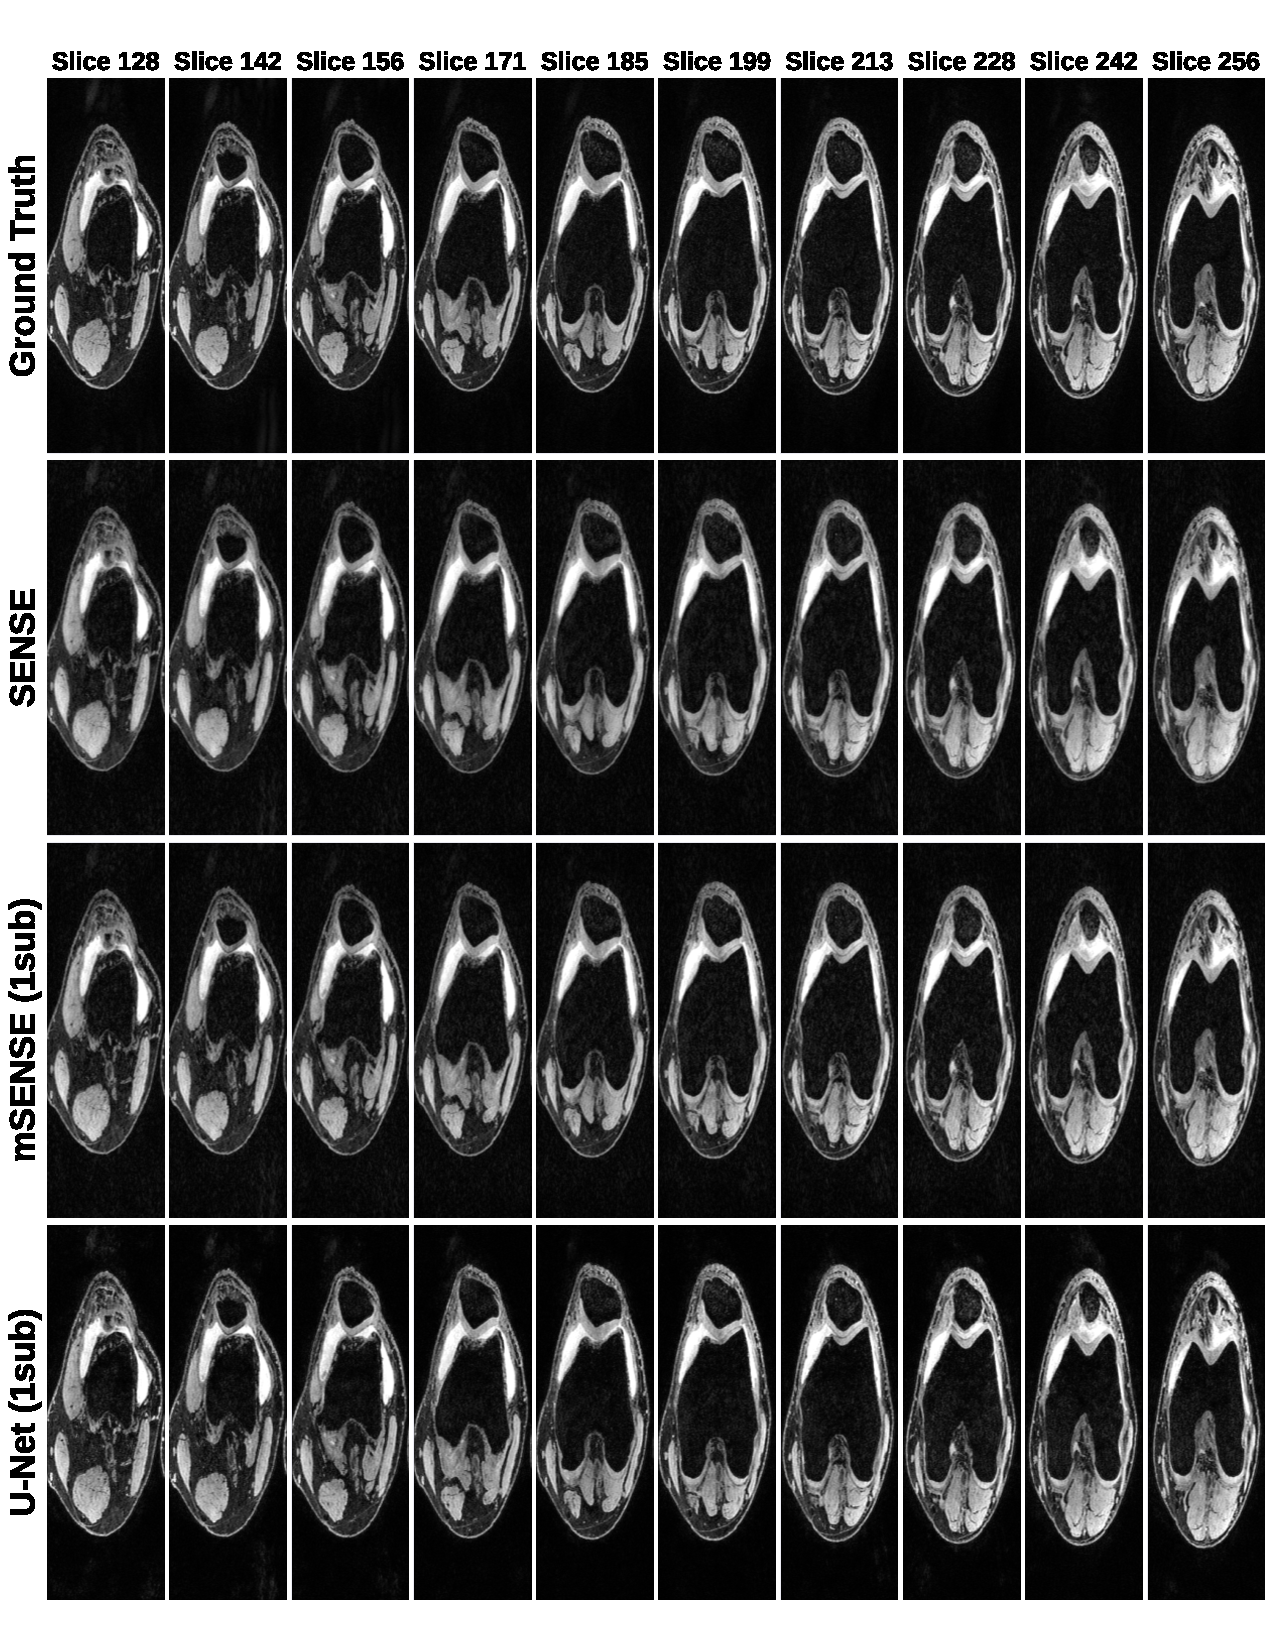
\includegraphics[width=0.9\linewidth]{figures/sample-mri-echo1.pdf}
    \vspace{-1em}
    \caption{Sample reconstructions at 2x acceleration for the first echo in the SKM-TEA dataset using SENSE, Monarch-SENSE (mSENSE), and U-Net. Both mSENSE and U-Net are trained with 1 training scan. SENSE is an untrained method.}
    \label{fig:mri-data-limited-echo1}
\end{figure}

\begin{figure}
    \centering
    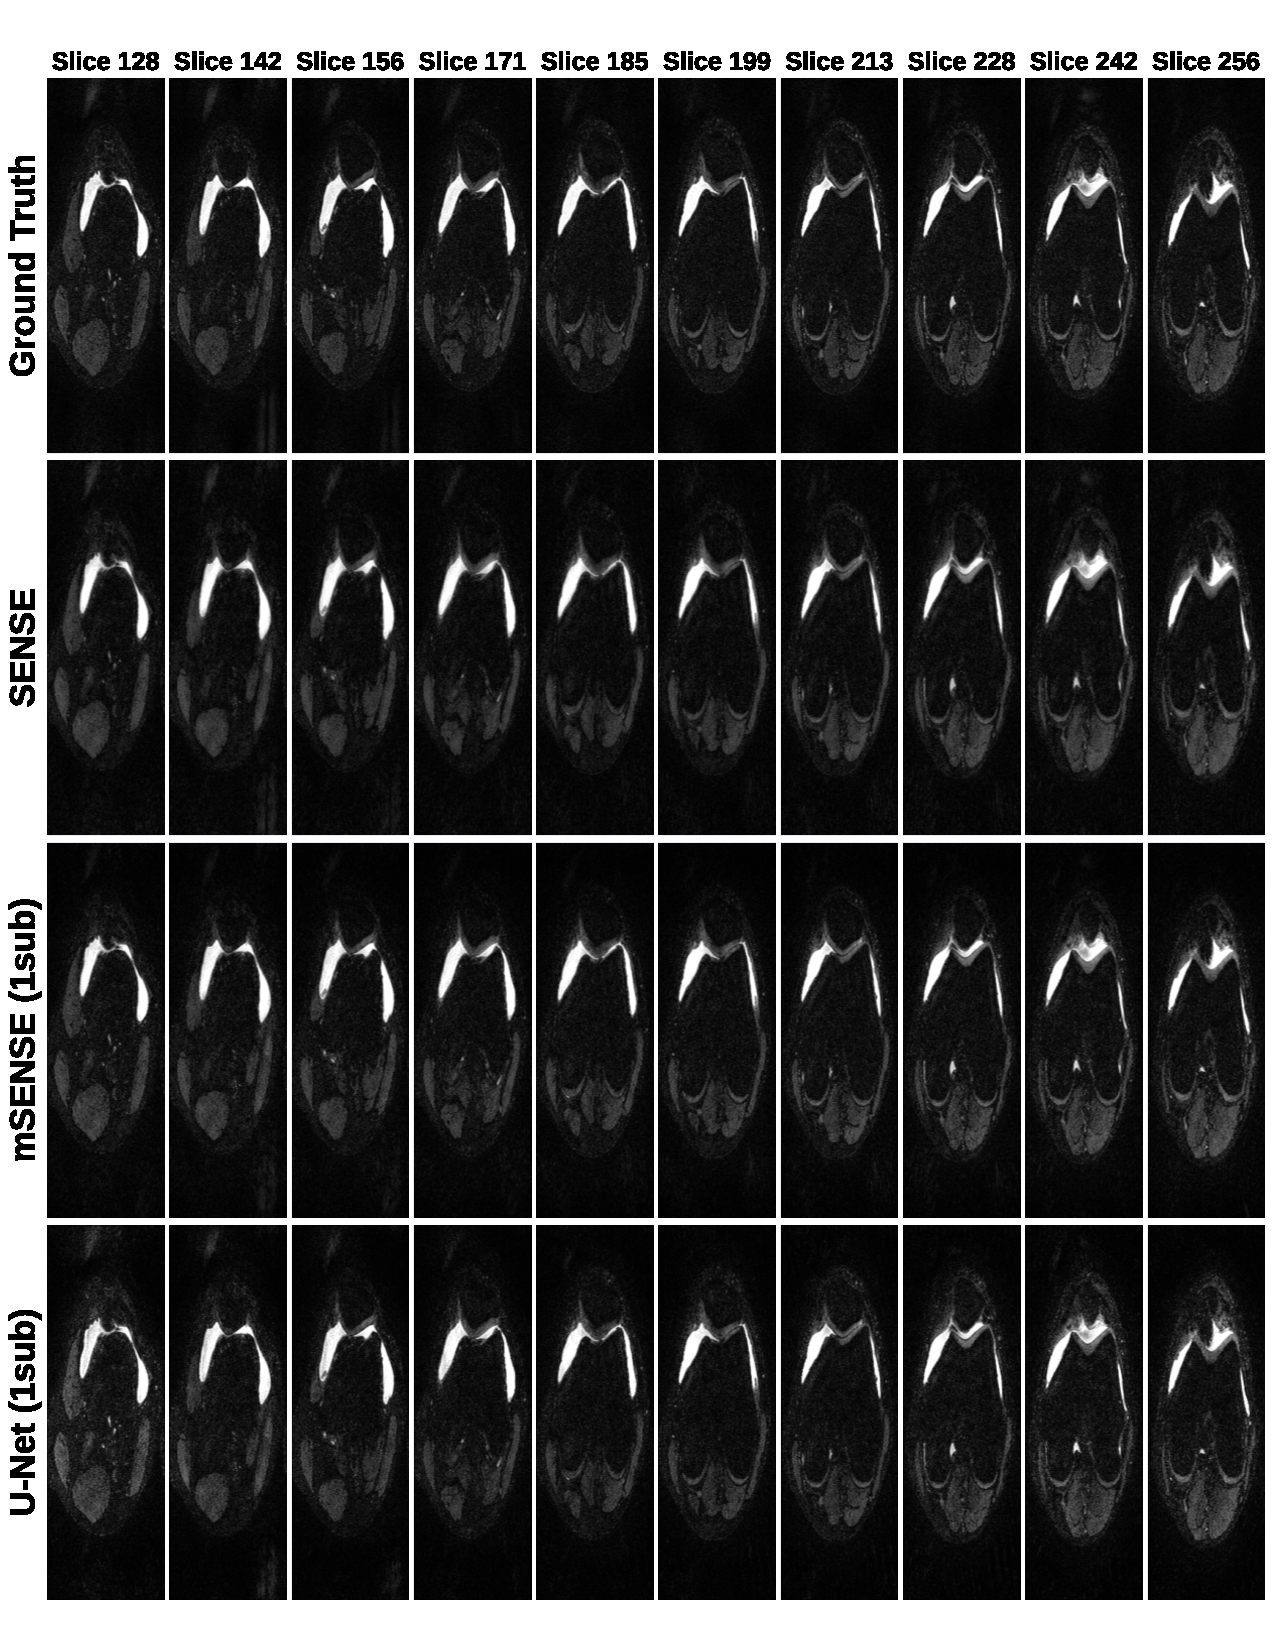
\includegraphics[width=6in]{figures/sample-mri-echo2.pdf}
    \vspace{-1em}
    \caption{Sample reconstructions at 2x acceleration for the second echo in the SKM-TEA dataset using SENSE, Monarch SENSE (mSENSE), and U-Net. Both mSENSE and U-Net are trained with 1 training scan. SENSE is an untrained method.}
    \label{fig:mri-data-limited-echo2}
\end{figure}








\end{document}
